\documentclass[10pt,aspectratio=169]{beamer}

% --- Theme & colours ---------------------------------------------------------
\usetheme{Madrid}
\usecolortheme{whale}
\useinnertheme{rectangles}
\setbeamertemplate{navigation symbols}{}
\setbeamertemplate{caption}[numbered]
\setbeamerfont{caption}{size=\scriptsize}
\setbeamercolor{block title}{bg=blue!15!white,fg=blue!50!black}
\setbeamercolor{block body}{bg=blue!5!white}

% --- Packages ----------------------------------------------------------------
\usepackage[utf8]{inputenc}
\usepackage[T1]{fontenc}
\usepackage{lmodern}
\usepackage{microtype}
\usepackage{graphicx}
\usepackage{booktabs}
\usepackage{amsmath,amssymb}
\usepackage{xcolor}
\usepackage{caption}
\usepackage{subcaption}

\graphicspath{{images/}}

% --- Title block -------------------------------------------------------------
\title[MACE Risk Prediction]{Predicting Major Adverse Cardiovascular Events\\
from a Baseline Proteomic Panel}
\subtitle{A stability-selected, nested-cross-validated, multi-model pipeline\\
(Random Forest, XGBoost, Logistic Regression, SVM-RBF)}
\author[M. Mohseni]{Mahdi Mohseni \\ \scriptsize Supervisor: Steven Watterson}
\institute[]{MACE Risk-Prediction Project}
\date{\today}

\begin{document}

% =============================================================================
\begin{frame}
  \titlepage
\end{frame}

% =============================================================================
\begin{frame}{Outline}
  \tableofcontents
\end{frame}

% =============================================================================
\section{Motivation}

\begin{frame}{What is MACE?}
  \begin{block}{MACE = Major Adverse Cardiovascular Events}
    A composite clinical endpoint, typically including:
    \begin{itemize}
      \item Cardiovascular death
      \item Non-fatal myocardial infarction (heart attack)
      \item Non-fatal stroke
      \item Unplanned coronary revascularisation
    \end{itemize}
  \end{block}
  \begin{itemize}
    \item Used as the headline outcome in cardiology trials and
          large-scale cardiovascular risk studies.
    \item In this project: a \textbf{binary} flag per patient per
          horizon -- did the patient experience any MACE component
          \emph{within} $k$ years of the index visit?
  \end{itemize}
\end{frame}

\begin{frame}{Why this project?}
  \begin{itemize}
    \item Cardiovascular disease is the \textbf{\#1 cause of mortality} worldwide.
    \item Existing risk scores (\textbf{EuroSCORE\,II, GRACE, SYNTAX})
          rely only on a handful of demographic and clinical variables.
    \item Modern \textbf{blood-based proteomic panels} (e.g.\ Olink) are
          mechanism-aware and increasingly affordable.
    \item Question: can we turn a $\sim$500-protein baseline panel into a
          \textbf{1--7 year MACE risk predictor}?
  \end{itemize}
  \begin{block}{The hard part}
    Small-$n$, high-$p$ medical ML: $n=94$ patients, $p=551$ candidate
    features. Overfitting and selection-induced optimism dominate naive
    approaches.
  \end{block}
\end{frame}

\begin{frame}{Research questions}
  \begin{itemize}
    \item \textbf{Q1 -- Predictability.} What unbiased, held-out
          performance is achievable for \emph{Within$k$Yr},
          $k\in\{1,\dots,7\}$?
    \item \textbf{Q2 -- Stability.} Which features are reproducibly
          selected across cross-validation folds?
    \item \textbf{Q3 -- Parsimony.} How many of the selected features
          actually carry the predictive signal?
  \end{itemize}
  \begin{block}{Headline horizon}
    We anchor this talk on \textbf{Within7Yr} -- the most balanced
    horizon (60\% positives), longest follow-up, and strongest results.
  \end{block}
\end{frame}

% =============================================================================
\section{Data and survival profile}

\begin{frame}{The cohort}
  \begin{columns}[T]
  \column{0.55\textwidth}
    \begin{itemize}
      \item $n=94$ patients
      \item $551$ numeric candidate features
            (Olink panels + derived analytes)
      \item Identifier: \texttt{EuroSCOREPatient ID} -- never used as a feature
      \item Seven binary outcomes:
            \texttt{Within1Yr}, $\dots$, \texttt{Within7Yr}
      \item Already imputed (no further missing-value handling)
    \end{itemize}
  \column{0.45\textwidth}
    \scriptsize
    \begin{tabular}{lrrr}
      \toprule
      Horizon & no MACE & MACE & Prev. \\
      \midrule
      Within1Yr & 77 & 17 & 0.18 \\
      Within2Yr & 62 & 32 & 0.34 \\
      Within3Yr & 58 & 36 & 0.38 \\
      Within4Yr & 51 & 43 & 0.46 \\
      Within5Yr & 47 & 47 & 0.50 \\
      Within6Yr & 41 & 53 & 0.56 \\
      \textbf{Within7Yr} & \textbf{38} & \textbf{56} & \textbf{0.60} \\
      \bottomrule
    \end{tabular}\\[2pt]
    \scriptsize Each row totals $n=94$ patients.
  \end{columns}
\end{frame}

\begin{frame}{Cohort survival profile}
  \begin{figure}
    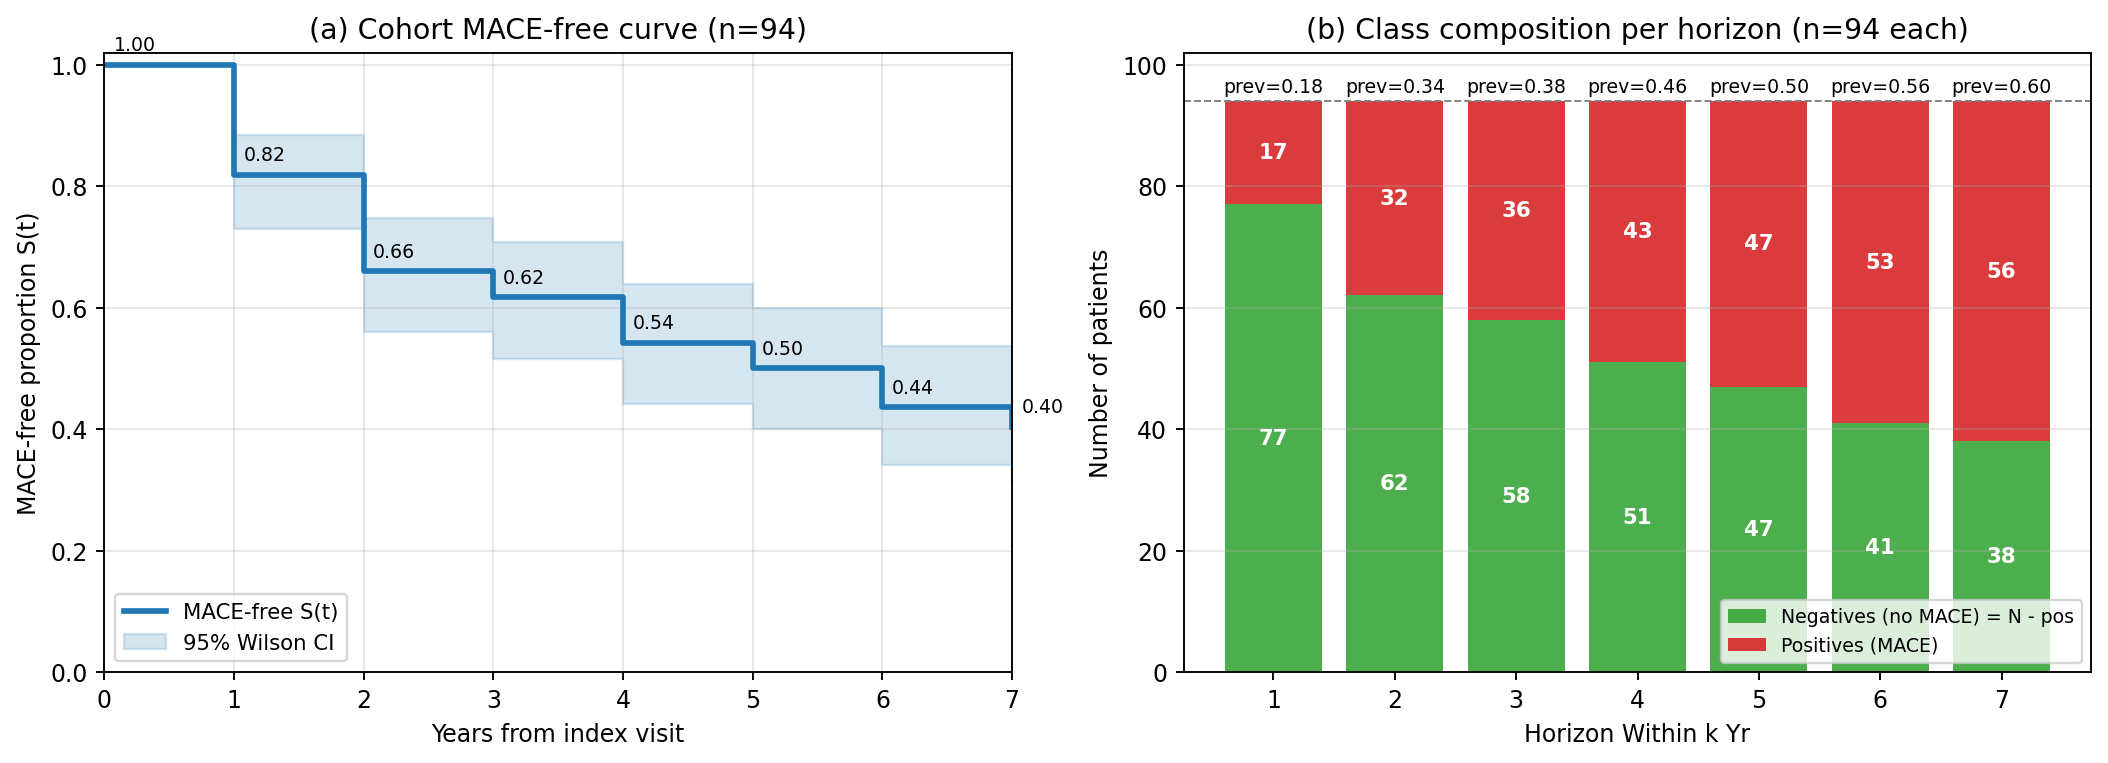
\includegraphics[width=0.92\textwidth]{survival_curve.png}
  \end{figure}
  \begin{itemize}
    \item Discrete-time MACE-free curve $S(k) = 1 - P(\mathrm{MACE}\le k)$.
    \item Sharp early drop (year 1: $S=0.82$); slower late decline ($S(7)=0.40$).
    \item Long horizons are the most class-balanced -- our headline analyses.
  \end{itemize}
\end{frame}

% =============================================================================
\section{Pipeline}

\begin{frame}{The pipeline at a glance}
  \begin{block}{Three guarded stages, four classifier families}
    \begin{enumerate}
      \item \textbf{Pre-processing} -- identifier / outcome handling, fold-aware standardisation.
      \item \textbf{Feature selection} -- stability selection over an $\ell_1$ regularisation grid.
      \item \textbf{Model + tuning} -- nested-CV grid search for each of:
        \emph{Random Forest, XGBoost, Logistic Regression, SVM-RBF}.
    \end{enumerate}
  \end{block}

  \begin{block}{Validation (identical across the four families)}
    \textbf{Outer:} \texttt{RepeatedStratifiedKFold(5,3)} $\Rightarrow$ 15
    held-out estimates per outcome.\\
    \textbf{Inner:} \texttt{StratifiedKFold(5)} for hyperparameter tuning.\\
    Same protocol for all 7 outcomes and all 4 families; single seed
    \texttt{RANDOM\_STATE = 42}. Only the classifier and its grid change.
  \end{block}
\end{frame}

\begin{frame}{Stage 1 -- Pre-processing}
  \begin{itemize}
    \item \textbf{Identifier:} \texttt{EuroSCOREPatient ID} stored as a
          record-only column, never read into the feature matrix.
    \item \textbf{Outcomes:} only \texttt{Within$k$Yr} columns treated as
          targets; one binary classifier trained per horizon.
    \item \textbf{Per-target leakage prophylaxis:} when modelling
          \texttt{Within$k$Yr}, the other six outcome columns are
          \emph{dropped from the feature matrix} (no short-horizon leak
          into long-horizon prediction).
    \item \textbf{Missingness:} pre-imputed before this stage; nothing
          inside the supervised pipeline learns from full-data statistics.
    \item \textbf{Scaling:} \texttt{StandardScaler} fit \emph{inside every
          outer training fold only}, applied just for stability selection
          (Random Forest is scale-invariant).
  \end{itemize}
  \begin{block}{Why this matters}
    Every step that learns from data is fold-respecting; this is what
    makes the held-out estimates honest.
  \end{block}
\end{frame}

\begin{frame}{Stage 2 -- Feature selection: stability selection}
  \begin{block}{The problem}
    With $p=551$ and $n=94$, a single sparse fit gives a feature list that
    depends on which patients are in the training set and which $\lambda$
    is chosen.
  \end{block}
  \textbf{Approach.} For every outer training fold:
  \begin{itemize}
    \item Take $B=100$ random subsamples at $75\%$ size.
    \item For each $C\in\{0.01, 0.1, 1.0\}$, fit class-balanced
          $\ell_1$-logistic (SAGA solver).
    \item For each feature $j$ record selection frequency
          $\pi_{j,C}$.
    \item Aggregate by \emph{maximum} across $C$:
          $s_j = \max_C \pi_{j,C}$.
    \item Keep features with $s_j \ge 0.60$ (floor 5, ceiling 50).
  \end{itemize}
  \begin{block}{Why max, not mean?}
    A feature is kept if it is reliably picked up at \emph{any} regularisation level
    -- the \emph{randomised lasso} variant (Meinshausen \& B\"uhlmann 2010).
  \end{block}
\end{frame}

\begin{frame}{Stage 3 -- Four classifier families, one protocol}
  \textbf{Why four families?} A single classifier on small-$n$ data is
  brittle. Comparing four families under the \emph{same} CV / selection /
  metrics isolates ``model'' from ``preprocessing''.
  \scriptsize
  \begin{center}
  \begin{tabular}{p{2.7cm}p{9.6cm}}
    \toprule
    Family & Grid \\
    \midrule
    Random Forest &
    \texttt{n\_estimators}$\in\{300\}$,
    \texttt{max\_depth}$\in\{\text{None},5\}$,
    \texttt{min\_samples\_leaf}$\in\{1,3\}$,
    \texttt{max\_features}$\in\{\sqrt{p},0.3\}$ \\[2pt]
    XGBoost &
    \texttt{n\_estimators}$\in\{200,400\}$,
    \texttt{max\_depth}$\in\{3,5\}$,
    \texttt{learning\_rate}$\in\{0.05,0.1\}$,
    \texttt{subsample}$=0.8$,
    \texttt{scale\_pos\_weight}$=n_-/n_+$ \\[2pt]
    Logistic Regression &
    Pipeline(\texttt{StandardScaler}, \texttt{LR}); $\ell_1$/$\ell_2$,
    \texttt{C}$\in\{0.01,0.1,1,10\}$, \texttt{class\_weight=balanced} \\[2pt]
    SVM (RBF) &
    Pipeline(\texttt{StandardScaler}, \texttt{SVC(rbf, prob=True)});
    \texttt{C}$\in\{0.1,1,10\}$, \texttt{gamma}$\in\{$\texttt{scale}$,0.01,0.1\}$ \\
    \bottomrule
  \end{tabular}
  \end{center}
  \begin{itemize}
    \item Class imbalance: \texttt{class\_weight=balanced} (RF/LR/SVM) or
          \texttt{scale\_pos\_weight} per fold (XGB).
    \item Tree models train on raw selected columns (scale-invariant);
          LR / SVM scale inside a Pipeline.
    \item Inner CV: \texttt{GridSearchCV(scoring="roc\_auc")}, refit=True.
  \end{itemize}
\end{frame}

% =============================================================================
\section{All seven classifiers}

\begin{frame}{One pipeline, seven horizons (RF anchor)}
  \begin{itemize}
    \item Same nested CV, same stability selection, same RF tuning grid
          for every horizon -- the only thing that changes is the label.
    \item Pooled out-of-fold AUC climbs monotonically with horizon, from
          $0.64$ (Within1Yr) to $0.72$ (Within7Yr).
    \item The longer horizons are easier because they are more
          class-balanced (\textbf{not} because the proteomic signal is
          stronger far into the future).
  \end{itemize}
  \begin{figure}
    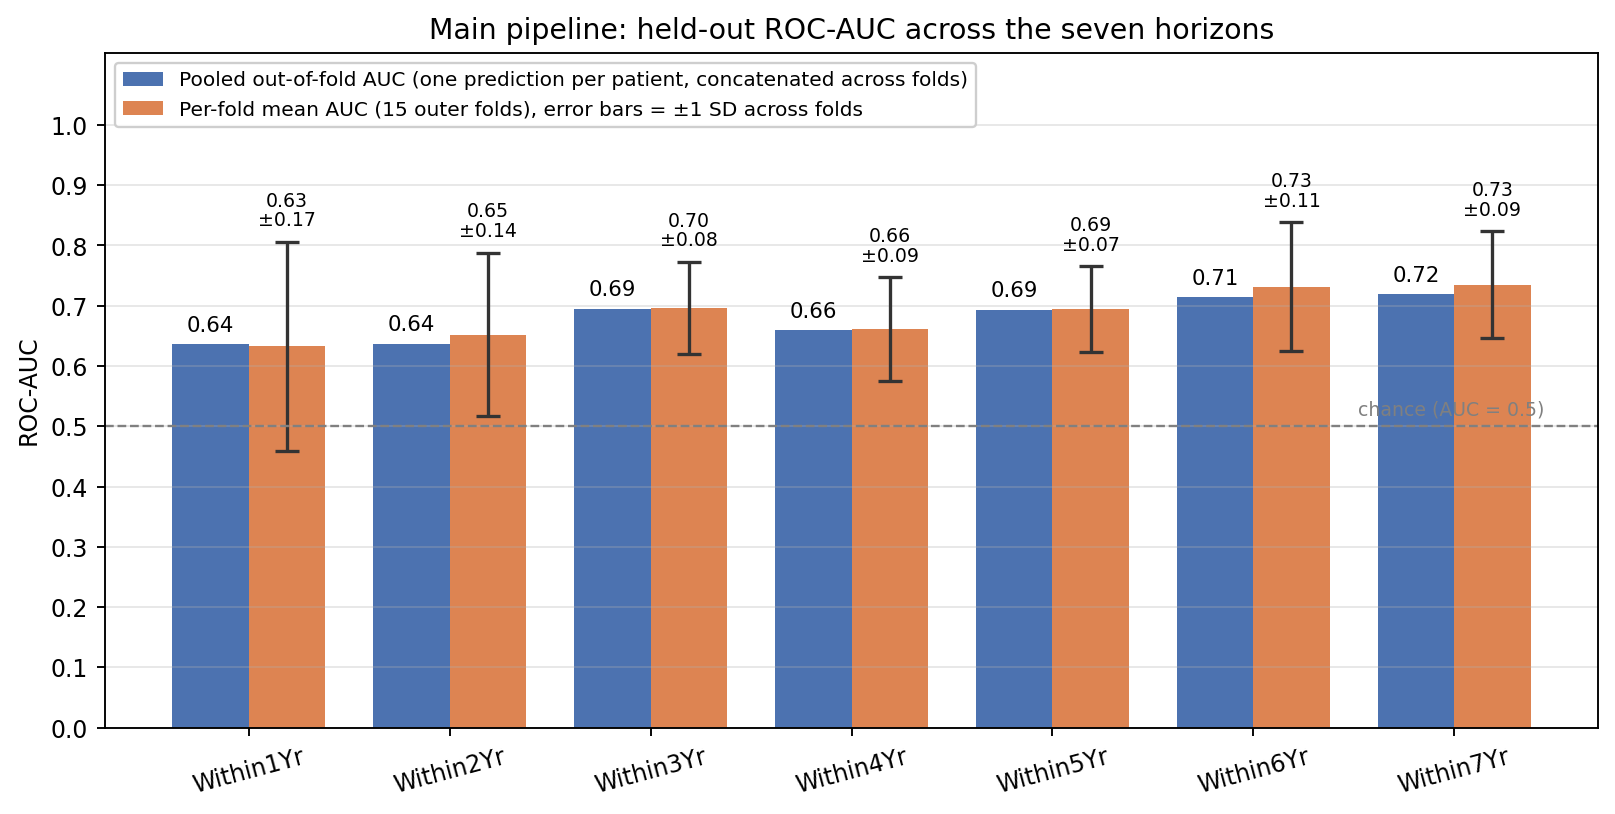
\includegraphics[width=0.78\textwidth]{compare_auc_horizons.png}
  \end{figure}
\end{frame}

% =============================================================================
\section{Cross-model comparison}

\begin{frame}{Four families, one protocol -- pooled AUC}
  \begin{columns}[T]
  \column{0.6\textwidth}
    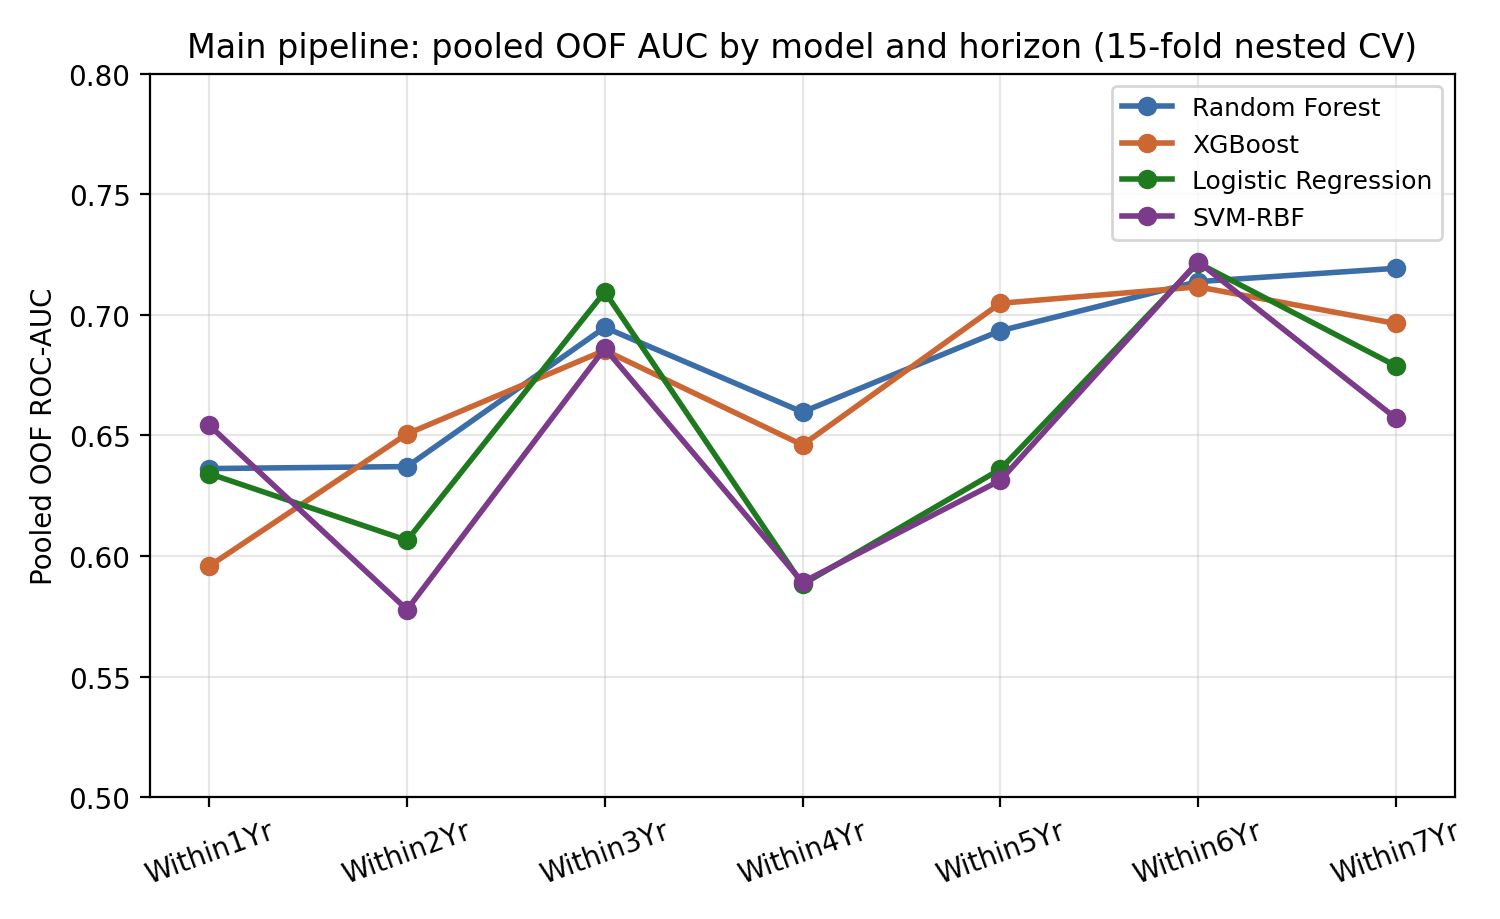
\includegraphics[width=\linewidth]{compare_models_pooled_auc.png}
  \column{0.4\textwidth}
    \begin{itemize}
      \item Spread across the four families at any horizon $\sim 0.06$ AUC.
      \item Smaller than the per-fold SD ($0.07$--$0.10$).
      \item \textbf{Tree models lead at the longer, more balanced
            horizons.}
      \item \textbf{Linear / kernel match RF on the imbalanced
            Within1Yr.}
      \item Headline performance is data-limited, not model-limited.
    \end{itemize}
  \end{columns}
\end{frame}

\begin{frame}{Cross-model balanced accuracy and Brier}
  \begin{columns}[T]
  \column{0.5\textwidth}
    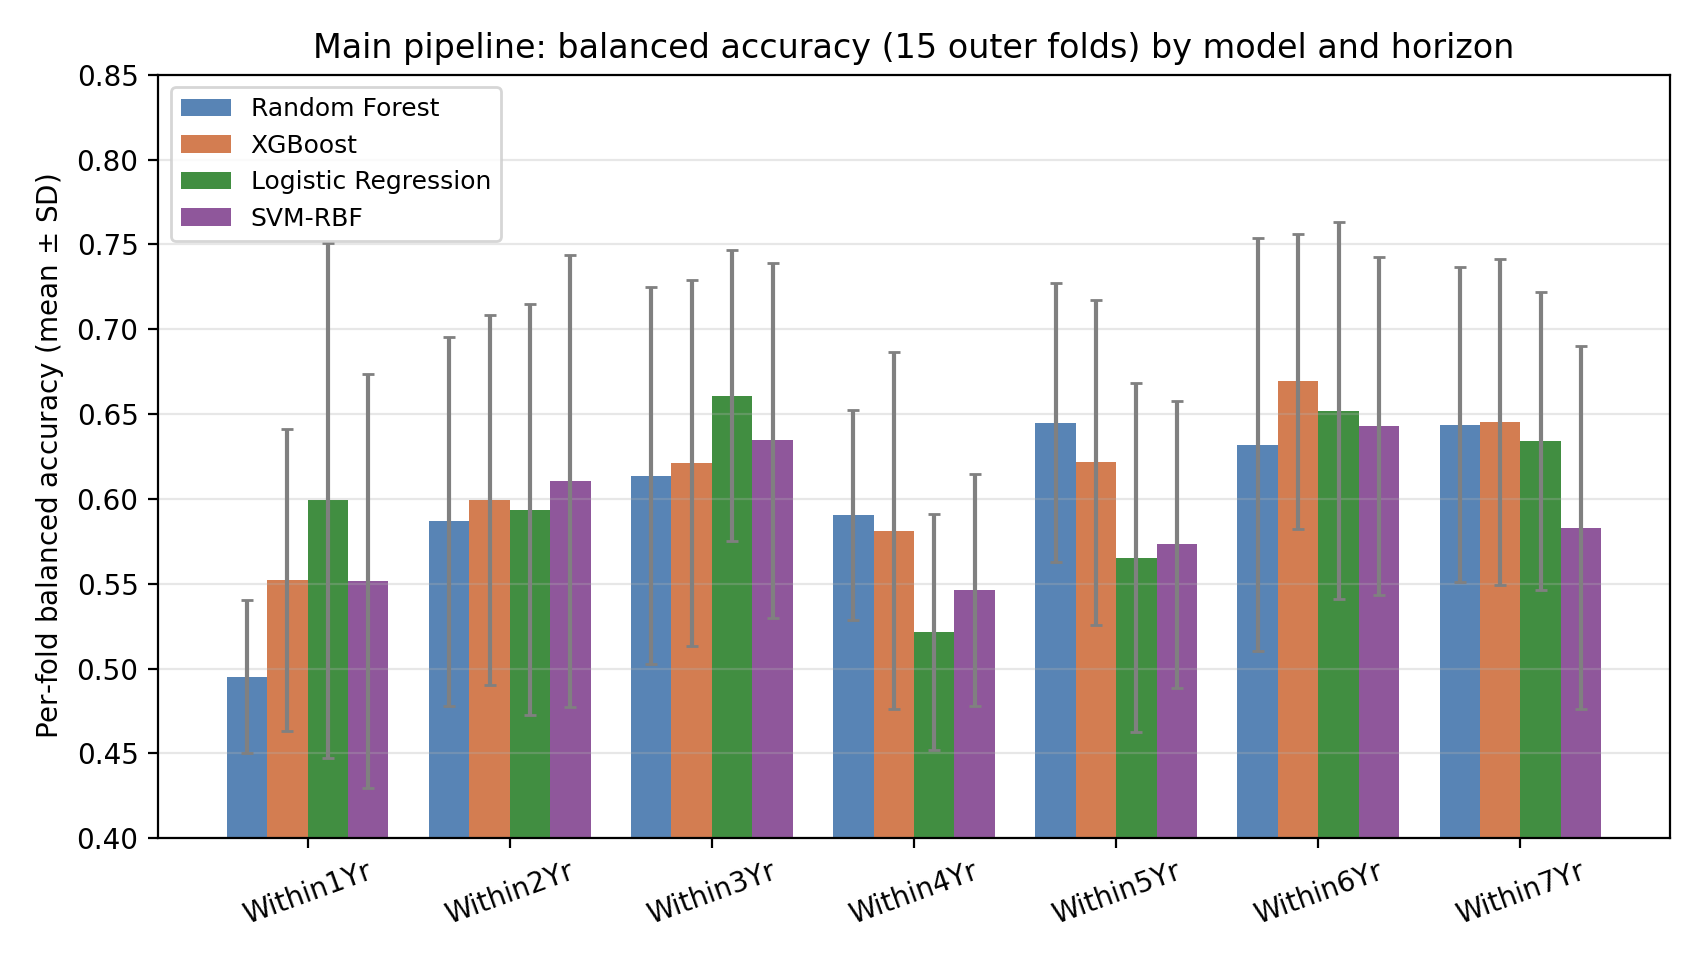
\includegraphics[width=\linewidth]{compare_models_balacc.png}
    \begin{center}\scriptsize Per-fold balanced accuracy (mean $\pm$ SD).\end{center}
  \column{0.5\textwidth}
    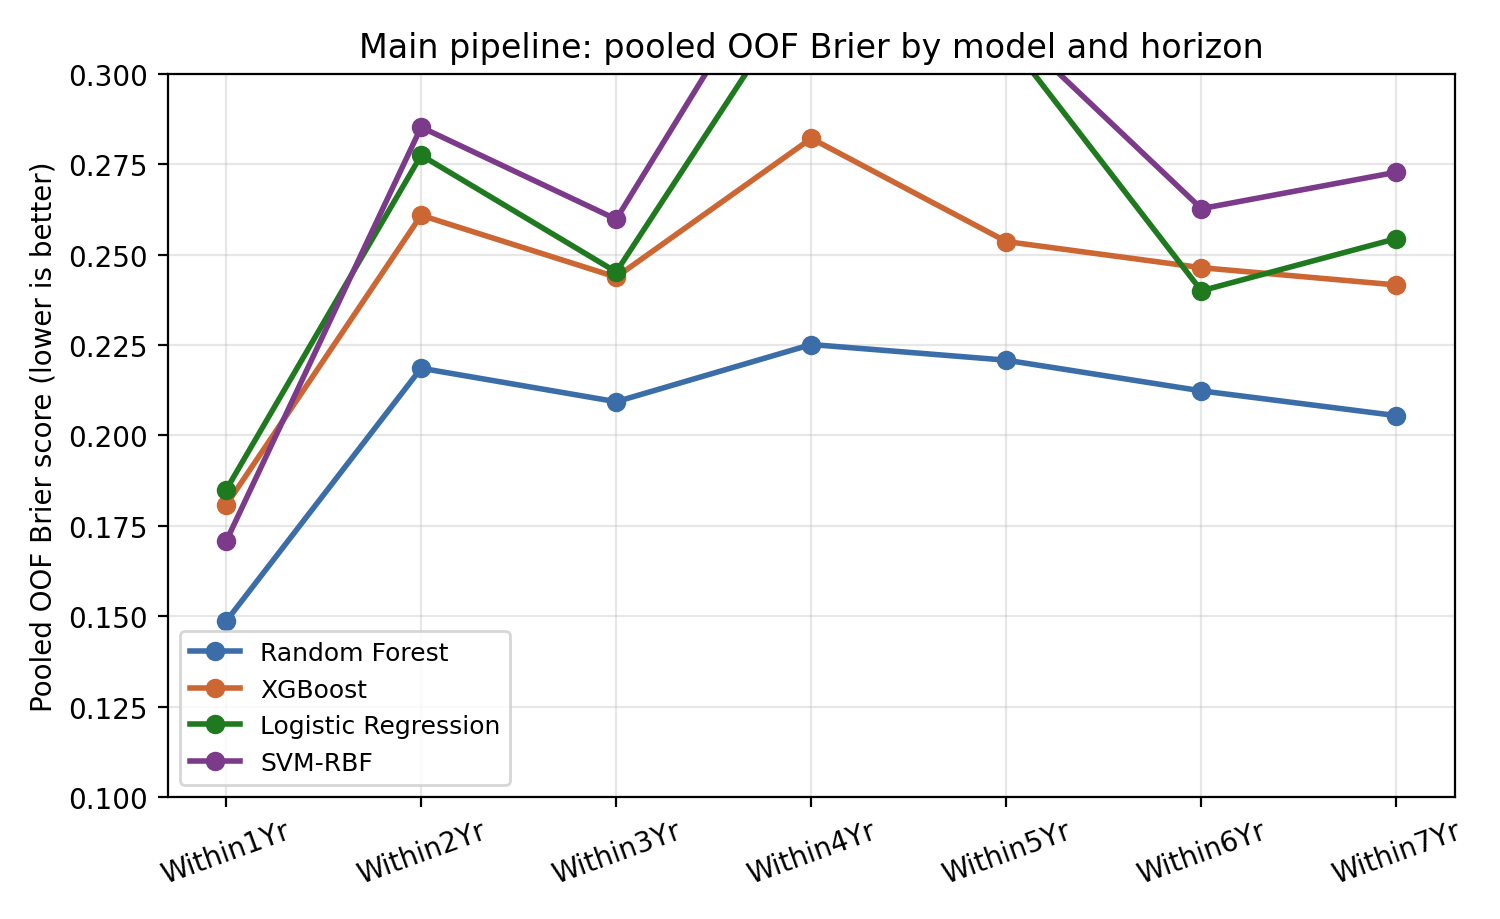
\includegraphics[width=\linewidth]{compare_models_brier.png}
    \begin{center}\scriptsize Pooled Brier (lower is better).\end{center}
  \end{columns}
  \begin{itemize}
    \item Tree-based families (RF, XGB) uniformly better calibrated.
    \item LR / SVM-RBF have similar AUC but worse Brier $\Rightarrow$
          would benefit from Platt / isotonic recalibration before
          deployment.
  \end{itemize}
\end{frame}

\begin{frame}{Cross-model headline numbers (representative horizons)}
  \scriptsize
  \begin{center}
  \begin{tabular}{llrrrrr}
    \toprule
    Horizon & Family & $|\mathcal{F}|$ & Pool. AUC & Pool. AP & BalAcc & Brier \\
    \midrule
    Within1Yr & Random Forest       & 33 & 0.636 & 0.286 & 0.495 & 0.149 \\
              & XGBoost             & 33 & 0.596 & 0.253 & 0.552 & 0.181 \\
              & Logistic Regression & 33 & 0.634 & 0.299 & 0.599 & 0.185 \\
              & SVM-RBF             & 33 & \textbf{0.654} & 0.292 & 0.552 & 0.171 \\
    \midrule
    Within3Yr & Random Forest       & 48 & 0.695 & 0.586 & 0.614 & 0.209 \\
              & XGBoost             & 48 & 0.685 & 0.591 & 0.621 & 0.244 \\
              & Logistic Regression & 48 & \textbf{0.710} & 0.622 & 0.661 & 0.245 \\
              & SVM-RBF             & 48 & 0.686 & 0.627 & 0.634 & 0.260 \\
    \midrule
    Within7Yr & Random Forest       & 49 & \textbf{0.719} & 0.792 & 0.644 & \textbf{0.205} \\
              & XGBoost             & 49 & 0.696 & 0.749 & 0.645 & 0.242 \\
              & Logistic Regression & 49 & 0.679 & 0.751 & 0.634 & 0.254 \\
              & SVM-RBF             & 49 & 0.657 & 0.758 & 0.583 & 0.273 \\
    \bottomrule
  \end{tabular}
  \end{center}
  \vspace{0.4em}
  \begin{itemize}
    \item RF wins Within7Yr; SVM-RBF wins Within1Yr; LR wins Within3Yr.
    \item All four within $\sim 0.06$ AUC of one another at every horizon.
  \end{itemize}
\end{frame}

\begin{frame}{Per-classifier highlights -- Within1Yr / Within2Yr}
  \begin{columns}[T]
  \column{0.5\textwidth}
    \textbf{Within1Yr} \scriptsize (prev 0.18, $|\mathcal{F}|=33$)
    \normalsize
    \begin{itemize}
      \item Pooled AUC \textbf{0.636}, BalAcc $\sim$0.50.
      \item Severely imbalanced -- defaults to majority at $\tau\!=\!0.5$.
      \item Youden cut recovers a usable operating point.
      \item Gradual peak AUC $0.87$ at $k\!=\!13$ (bumpy curve).
    \end{itemize}
    \vspace{0.4em}
    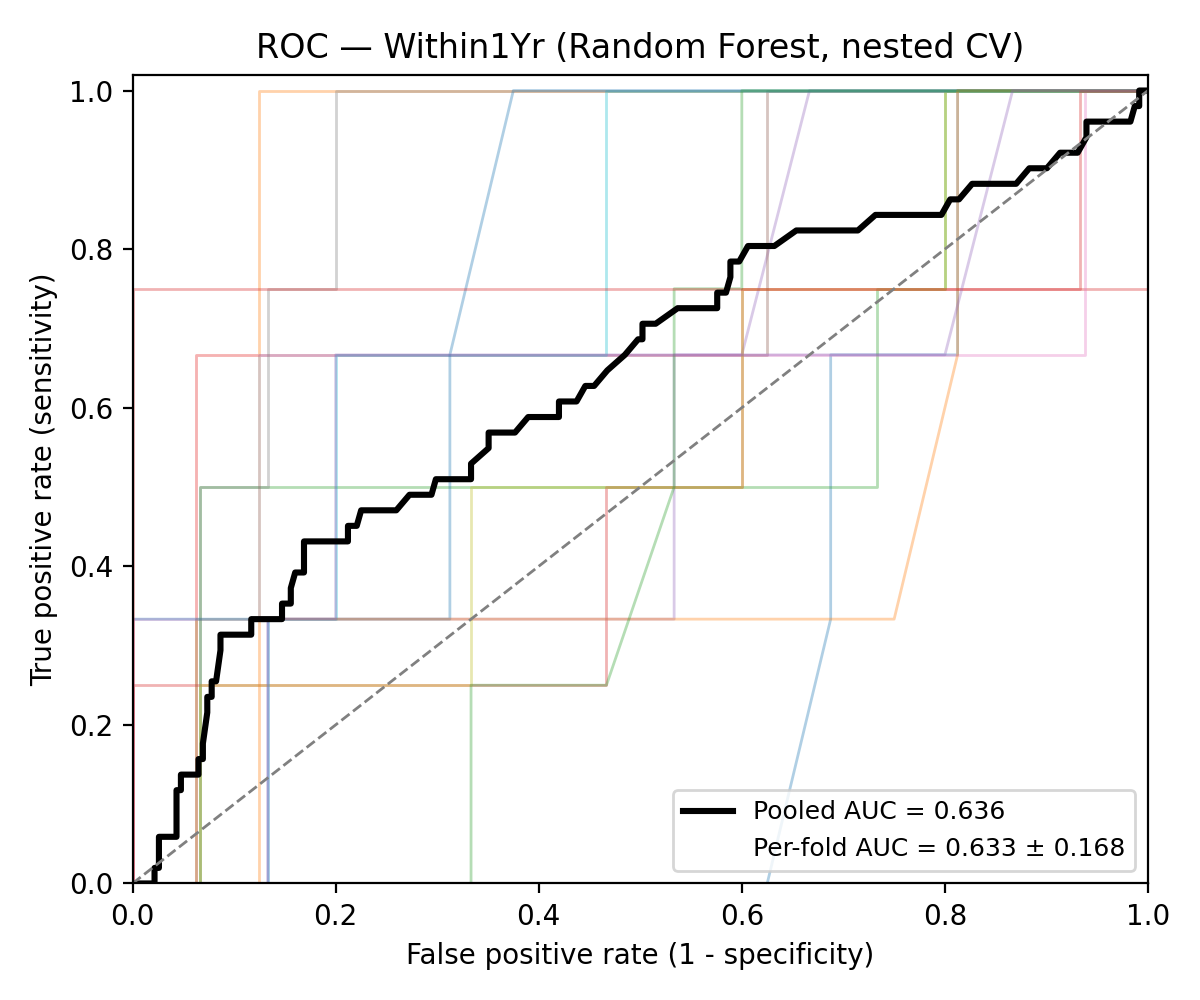
\includegraphics[width=\linewidth]{main_roc_within1yr.png}
  \column{0.5\textwidth}
    \textbf{Within2Yr} \scriptsize (prev 0.34, $|\mathcal{F}|=50$)
    \normalsize
    \begin{itemize}
      \item Pooled AUC \textbf{0.637}, BalAcc 0.59.
      \item Classes much closer to balanced.
      \item Gradual peak AUC $0.88$ at $k\!=\!42$.
    \end{itemize}
    \vspace{0.4em}
    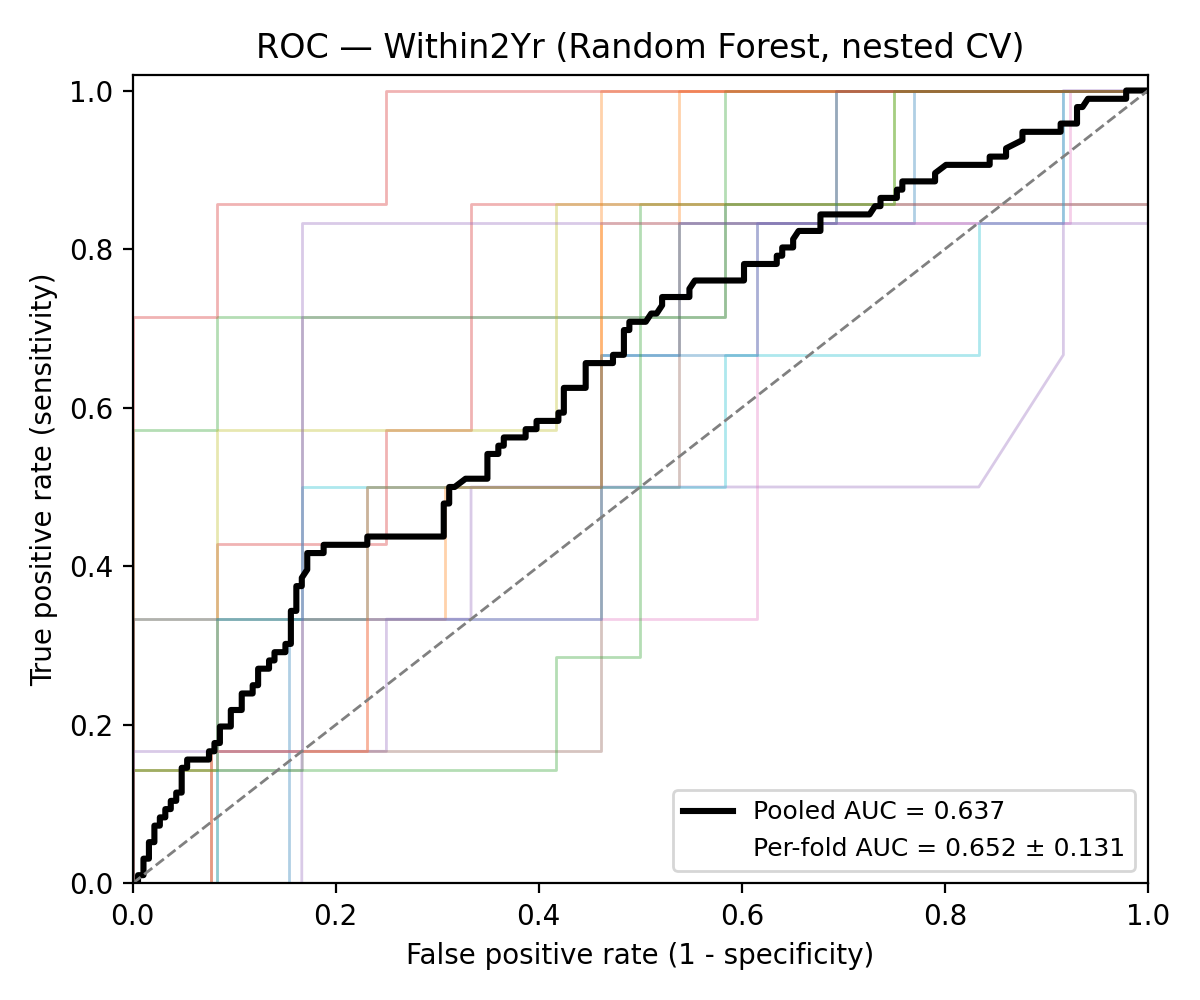
\includegraphics[width=\linewidth]{main_roc_within2yr.png}
  \end{columns}
\end{frame}

\begin{frame}{Per-classifier highlights -- Within3Yr / Within4Yr}
  \begin{columns}[T]
  \column{0.5\textwidth}
    \textbf{Within3Yr} \scriptsize (prev 0.38, $|\mathcal{F}|=48$)
    \normalsize
    \begin{itemize}
      \item Pooled AUC \textbf{0.695}, BalAcc 0.61.
      \item Gradual peak AUC \textbf{0.898} at $k\!=\!34$.
      \item First clearly above-chance pooled estimate.
    \end{itemize}
    \vspace{0.4em}
    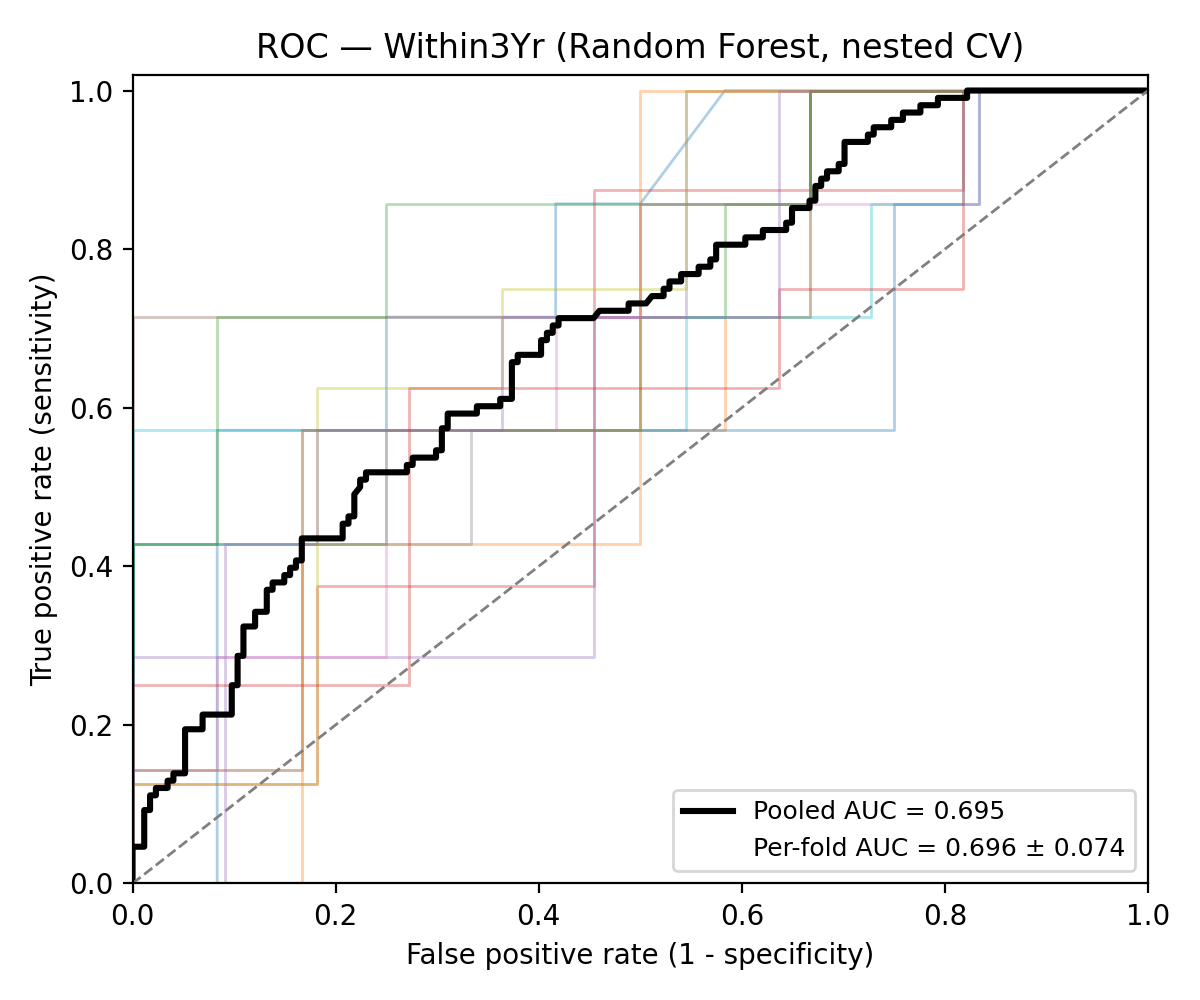
\includegraphics[width=\linewidth]{main_roc_within3yr.png}
  \column{0.5\textwidth}
    \textbf{Within4Yr} \scriptsize (prev 0.46, $|\mathcal{F}|=38$)
    \normalsize
    \begin{itemize}
      \item Pooled AUC \textbf{0.660}, BalAcc 0.59.
      \item Most stable BalAcc across folds ($\pm 0.06$).
      \item Gradual peak BalAcc \textbf{0.81} at $k\!=\!17$ -- the
            highest of any horizon.
    \end{itemize}
    \vspace{0.4em}
    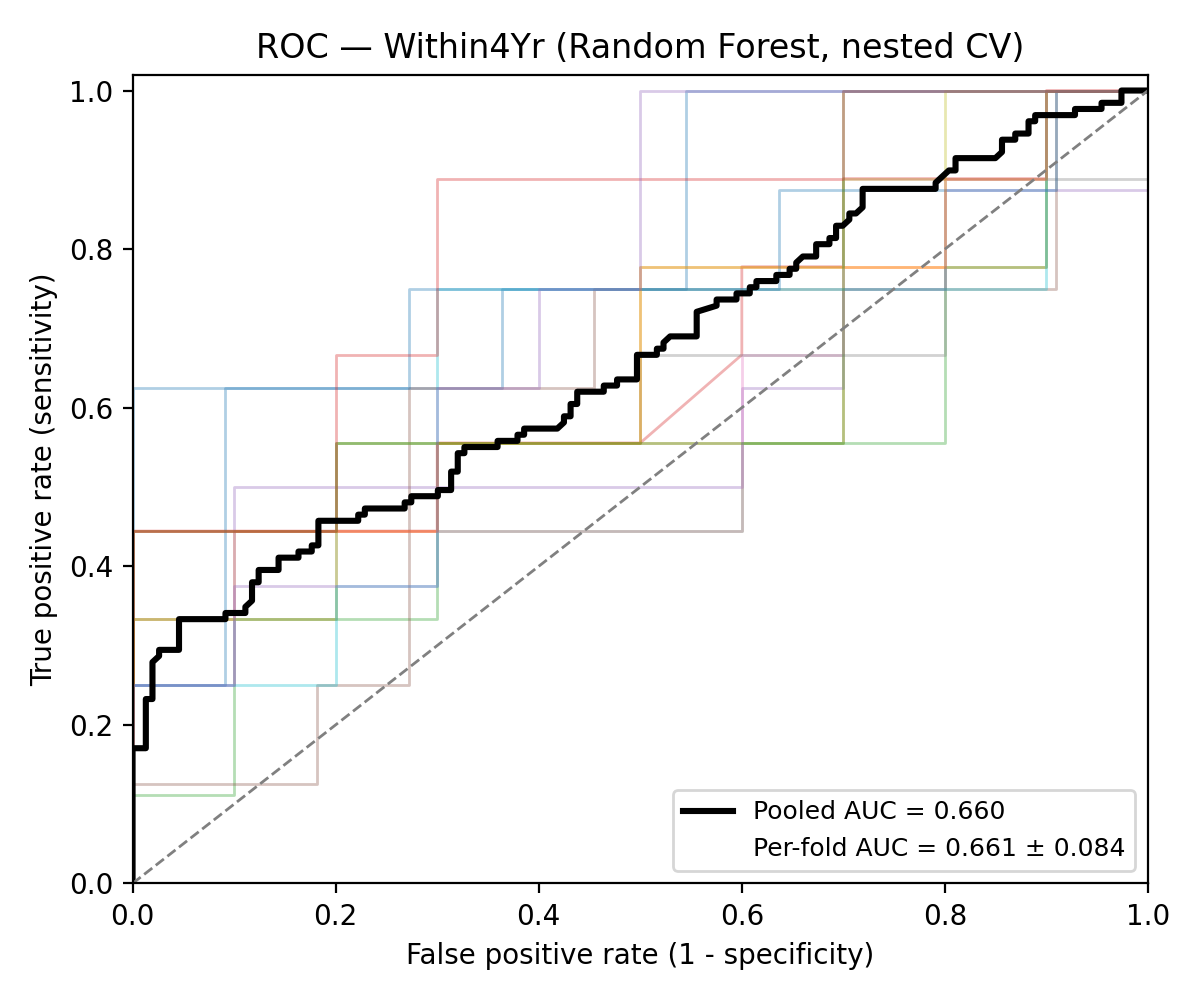
\includegraphics[width=\linewidth]{main_roc_within4yr.png}
  \end{columns}
\end{frame}

\begin{frame}{Per-classifier highlights -- Within5Yr / Within6Yr}
  \begin{columns}[T]
  \column{0.5\textwidth}
    \textbf{Within5Yr} \scriptsize (prev 0.50, $|\mathcal{F}|=46$)
    \normalsize
    \begin{itemize}
      \item Pooled AUC \textbf{0.693}, BalAcc 0.65.
      \item Best $k$ for BalAcc is just \textbf{8} -- the smallest of any
            horizon: a very compact subset already captures the signal.
    \end{itemize}
    \vspace{0.4em}
    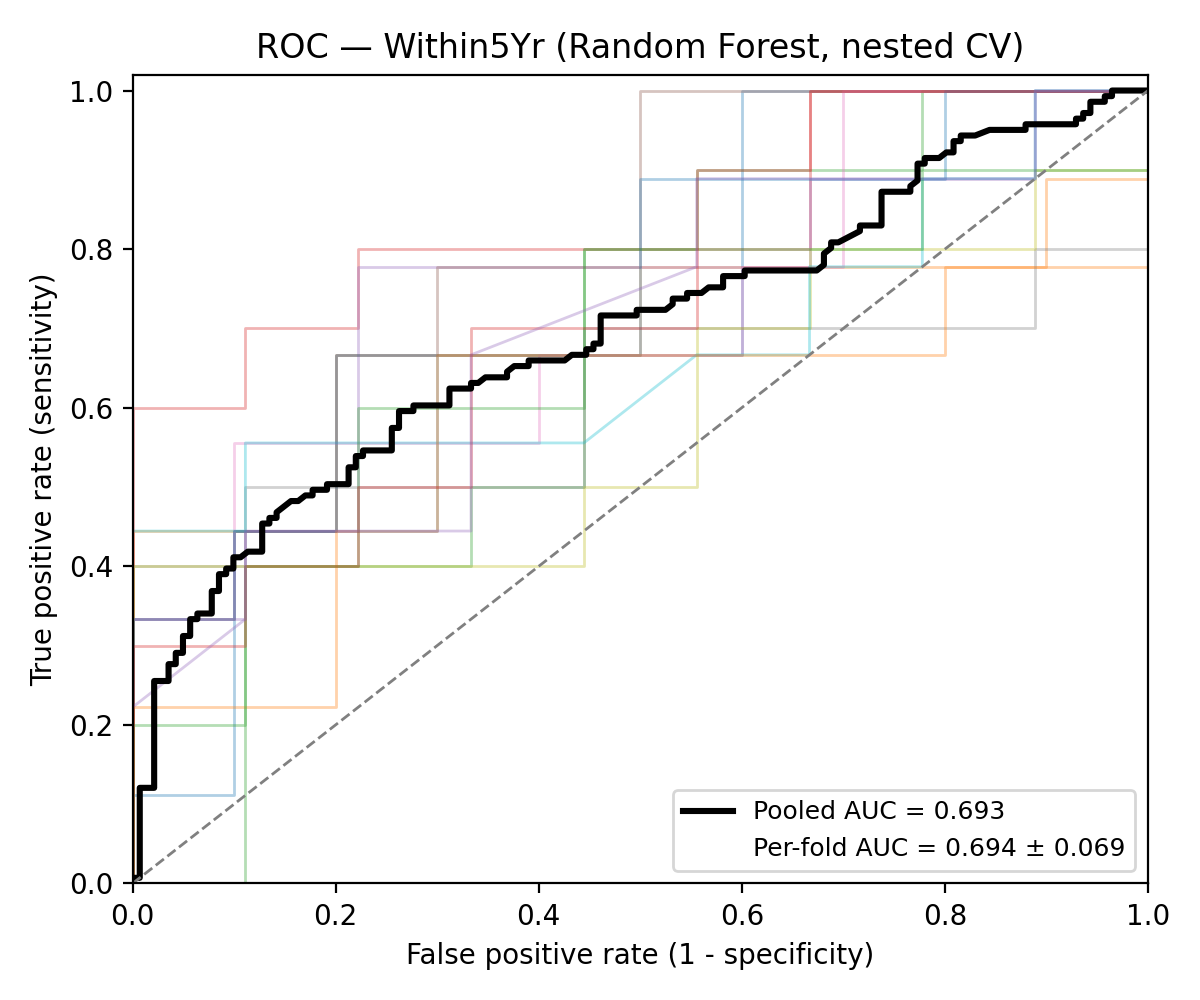
\includegraphics[width=\linewidth]{main_roc_within5yr.png}
  \column{0.5\textwidth}
    \textbf{Within6Yr} \scriptsize (prev 0.56, $|\mathcal{F}|=50$)
    \normalsize
    \begin{itemize}
      \item Pooled AUC \textbf{0.714}, BalAcc 0.63.
      \item Peak $F_1$ \textbf{0.82} at $k\!=\!13$.
      \item Closest competitor to Within7Yr.
    \end{itemize}
    \vspace{0.4em}
    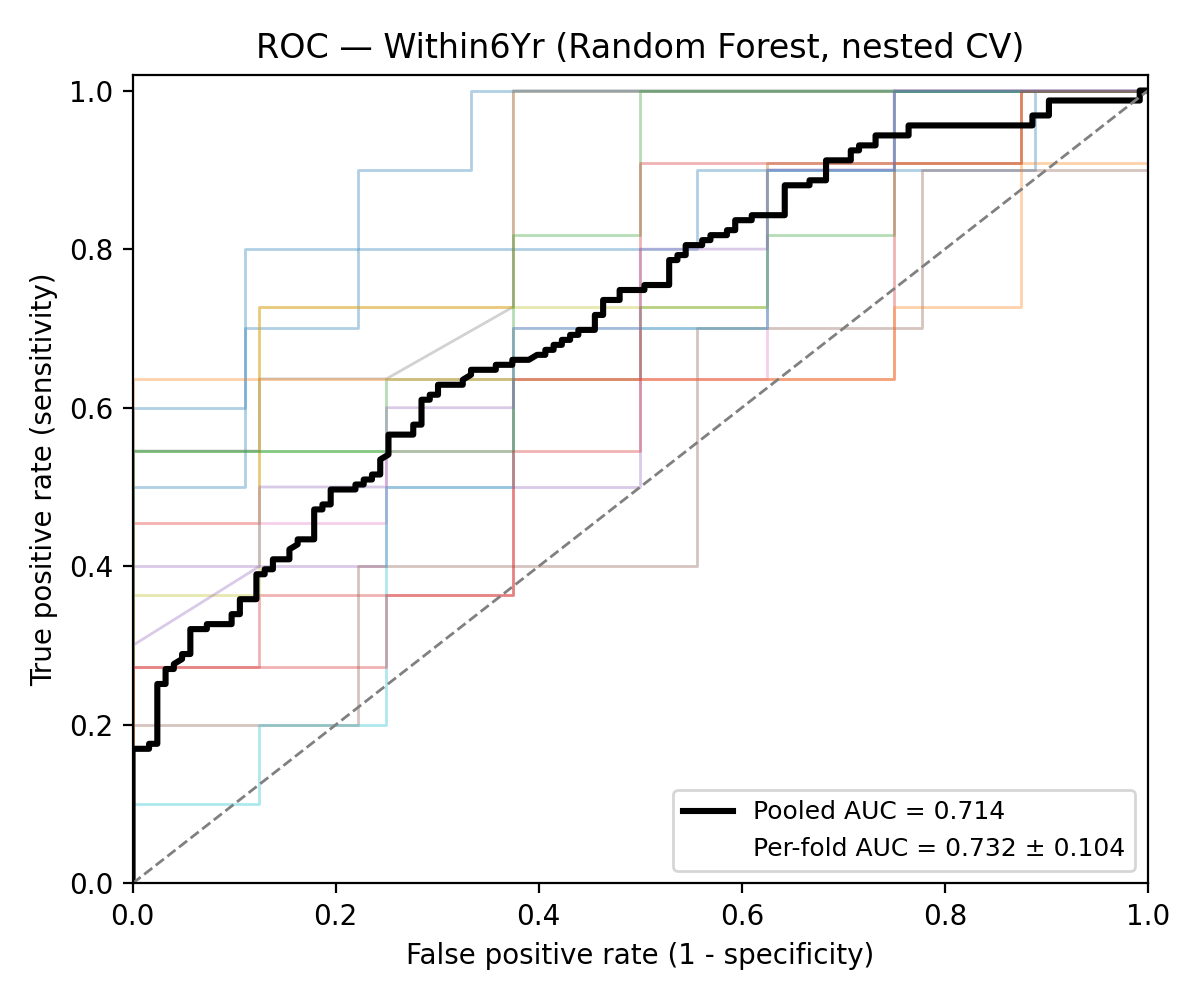
\includegraphics[width=\linewidth]{main_roc_within6yr.png}
  \end{columns}
\end{frame}

\begin{frame}{Gradual all-metric panels (Within1Yr -- Within6Yr)}
  \begin{columns}[T]
  \column{0.33\textwidth}
    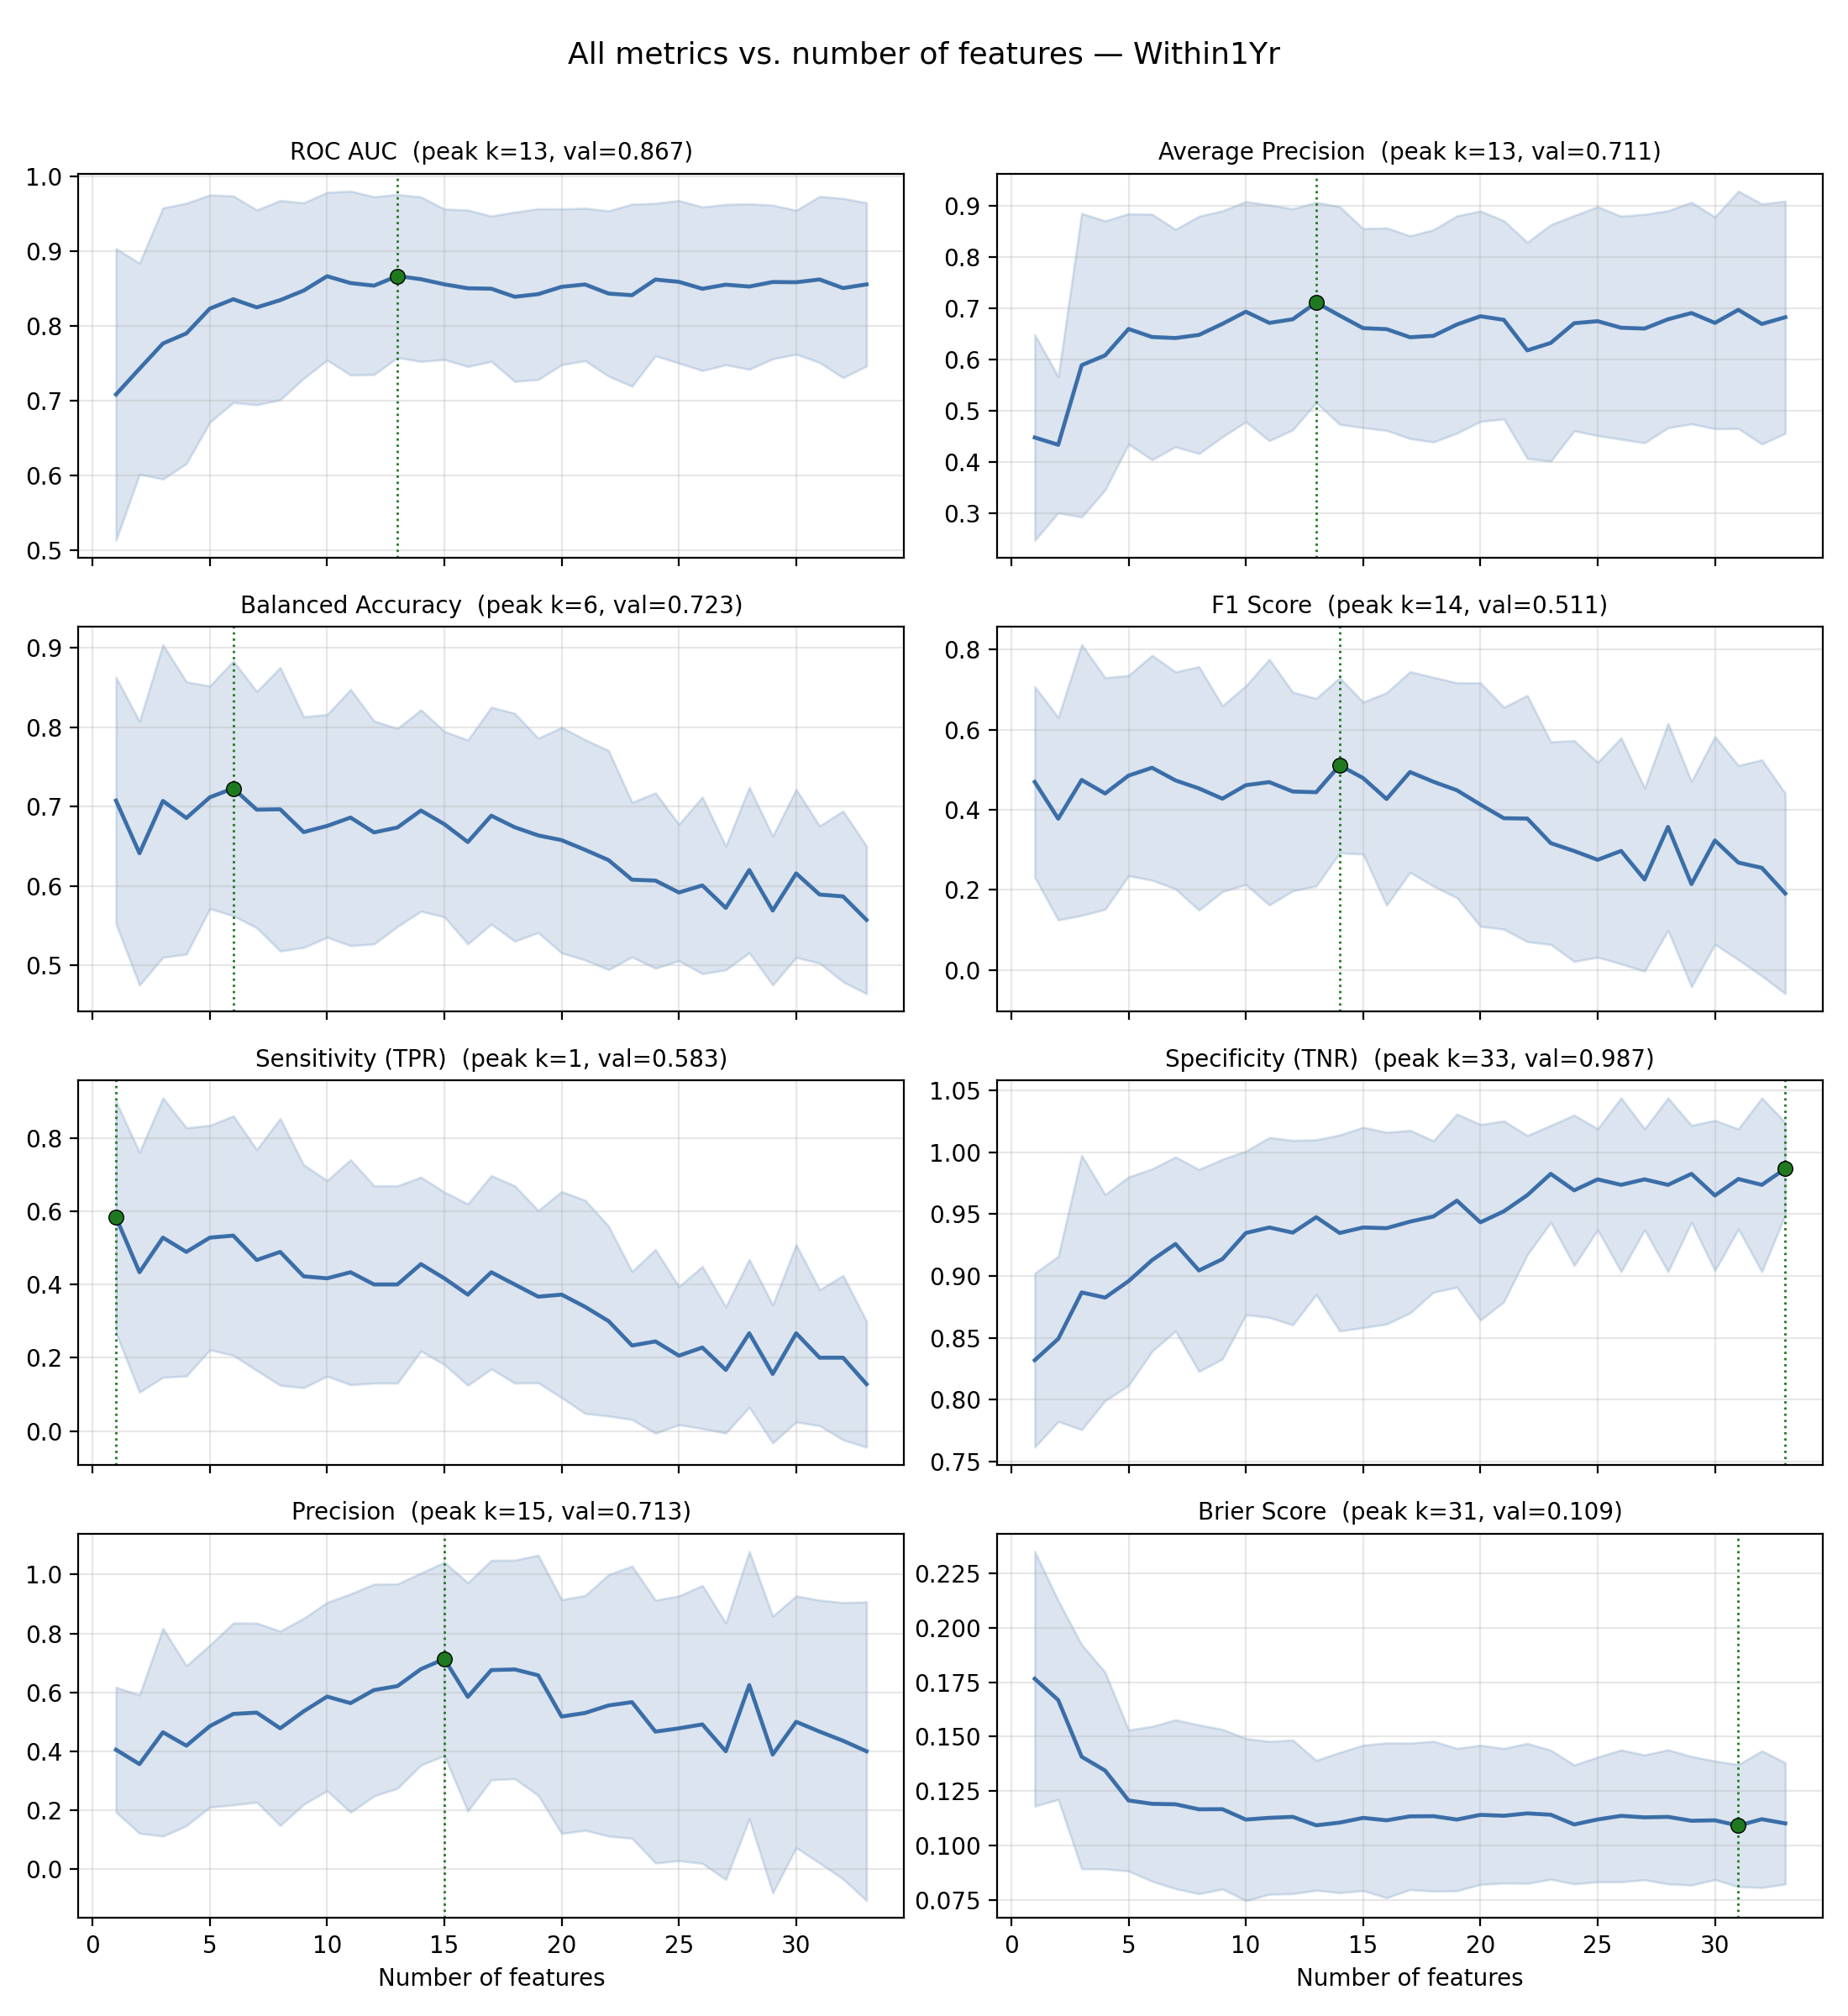
\includegraphics[width=\linewidth]{gradual_allmetrics_within1yr.png}\\
    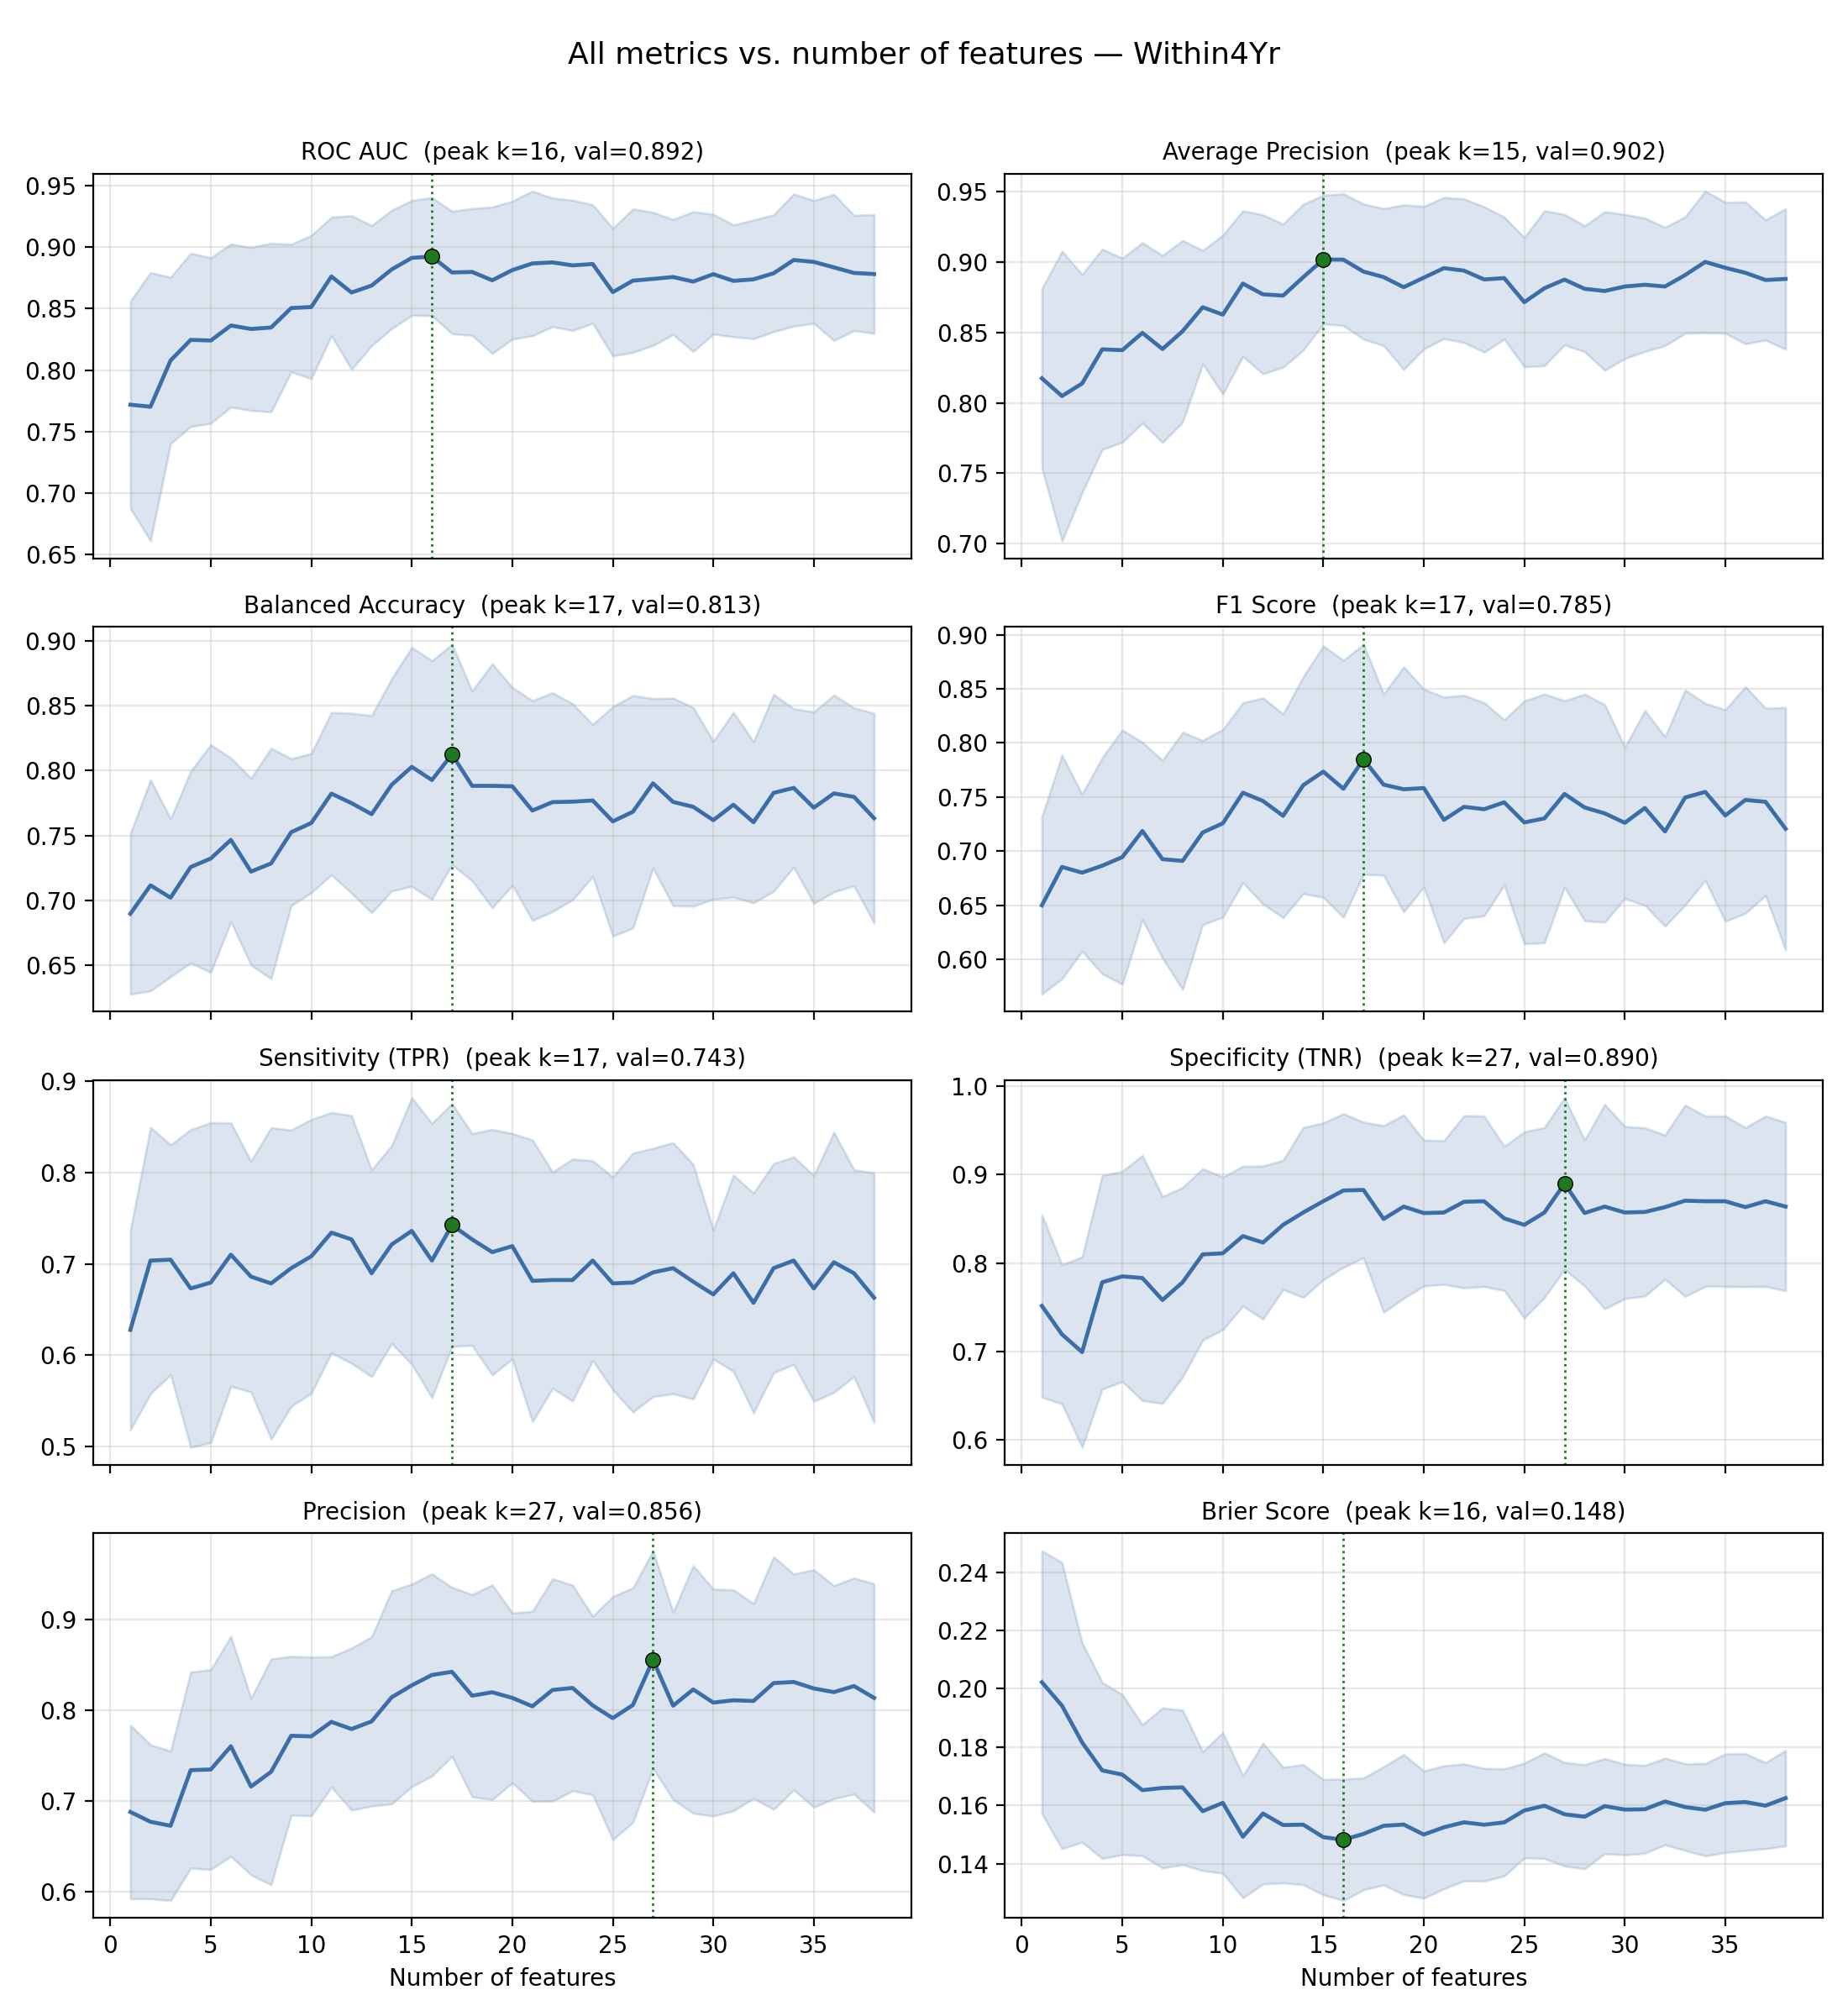
\includegraphics[width=\linewidth]{gradual_allmetrics_within4yr.png}
  \column{0.33\textwidth}
    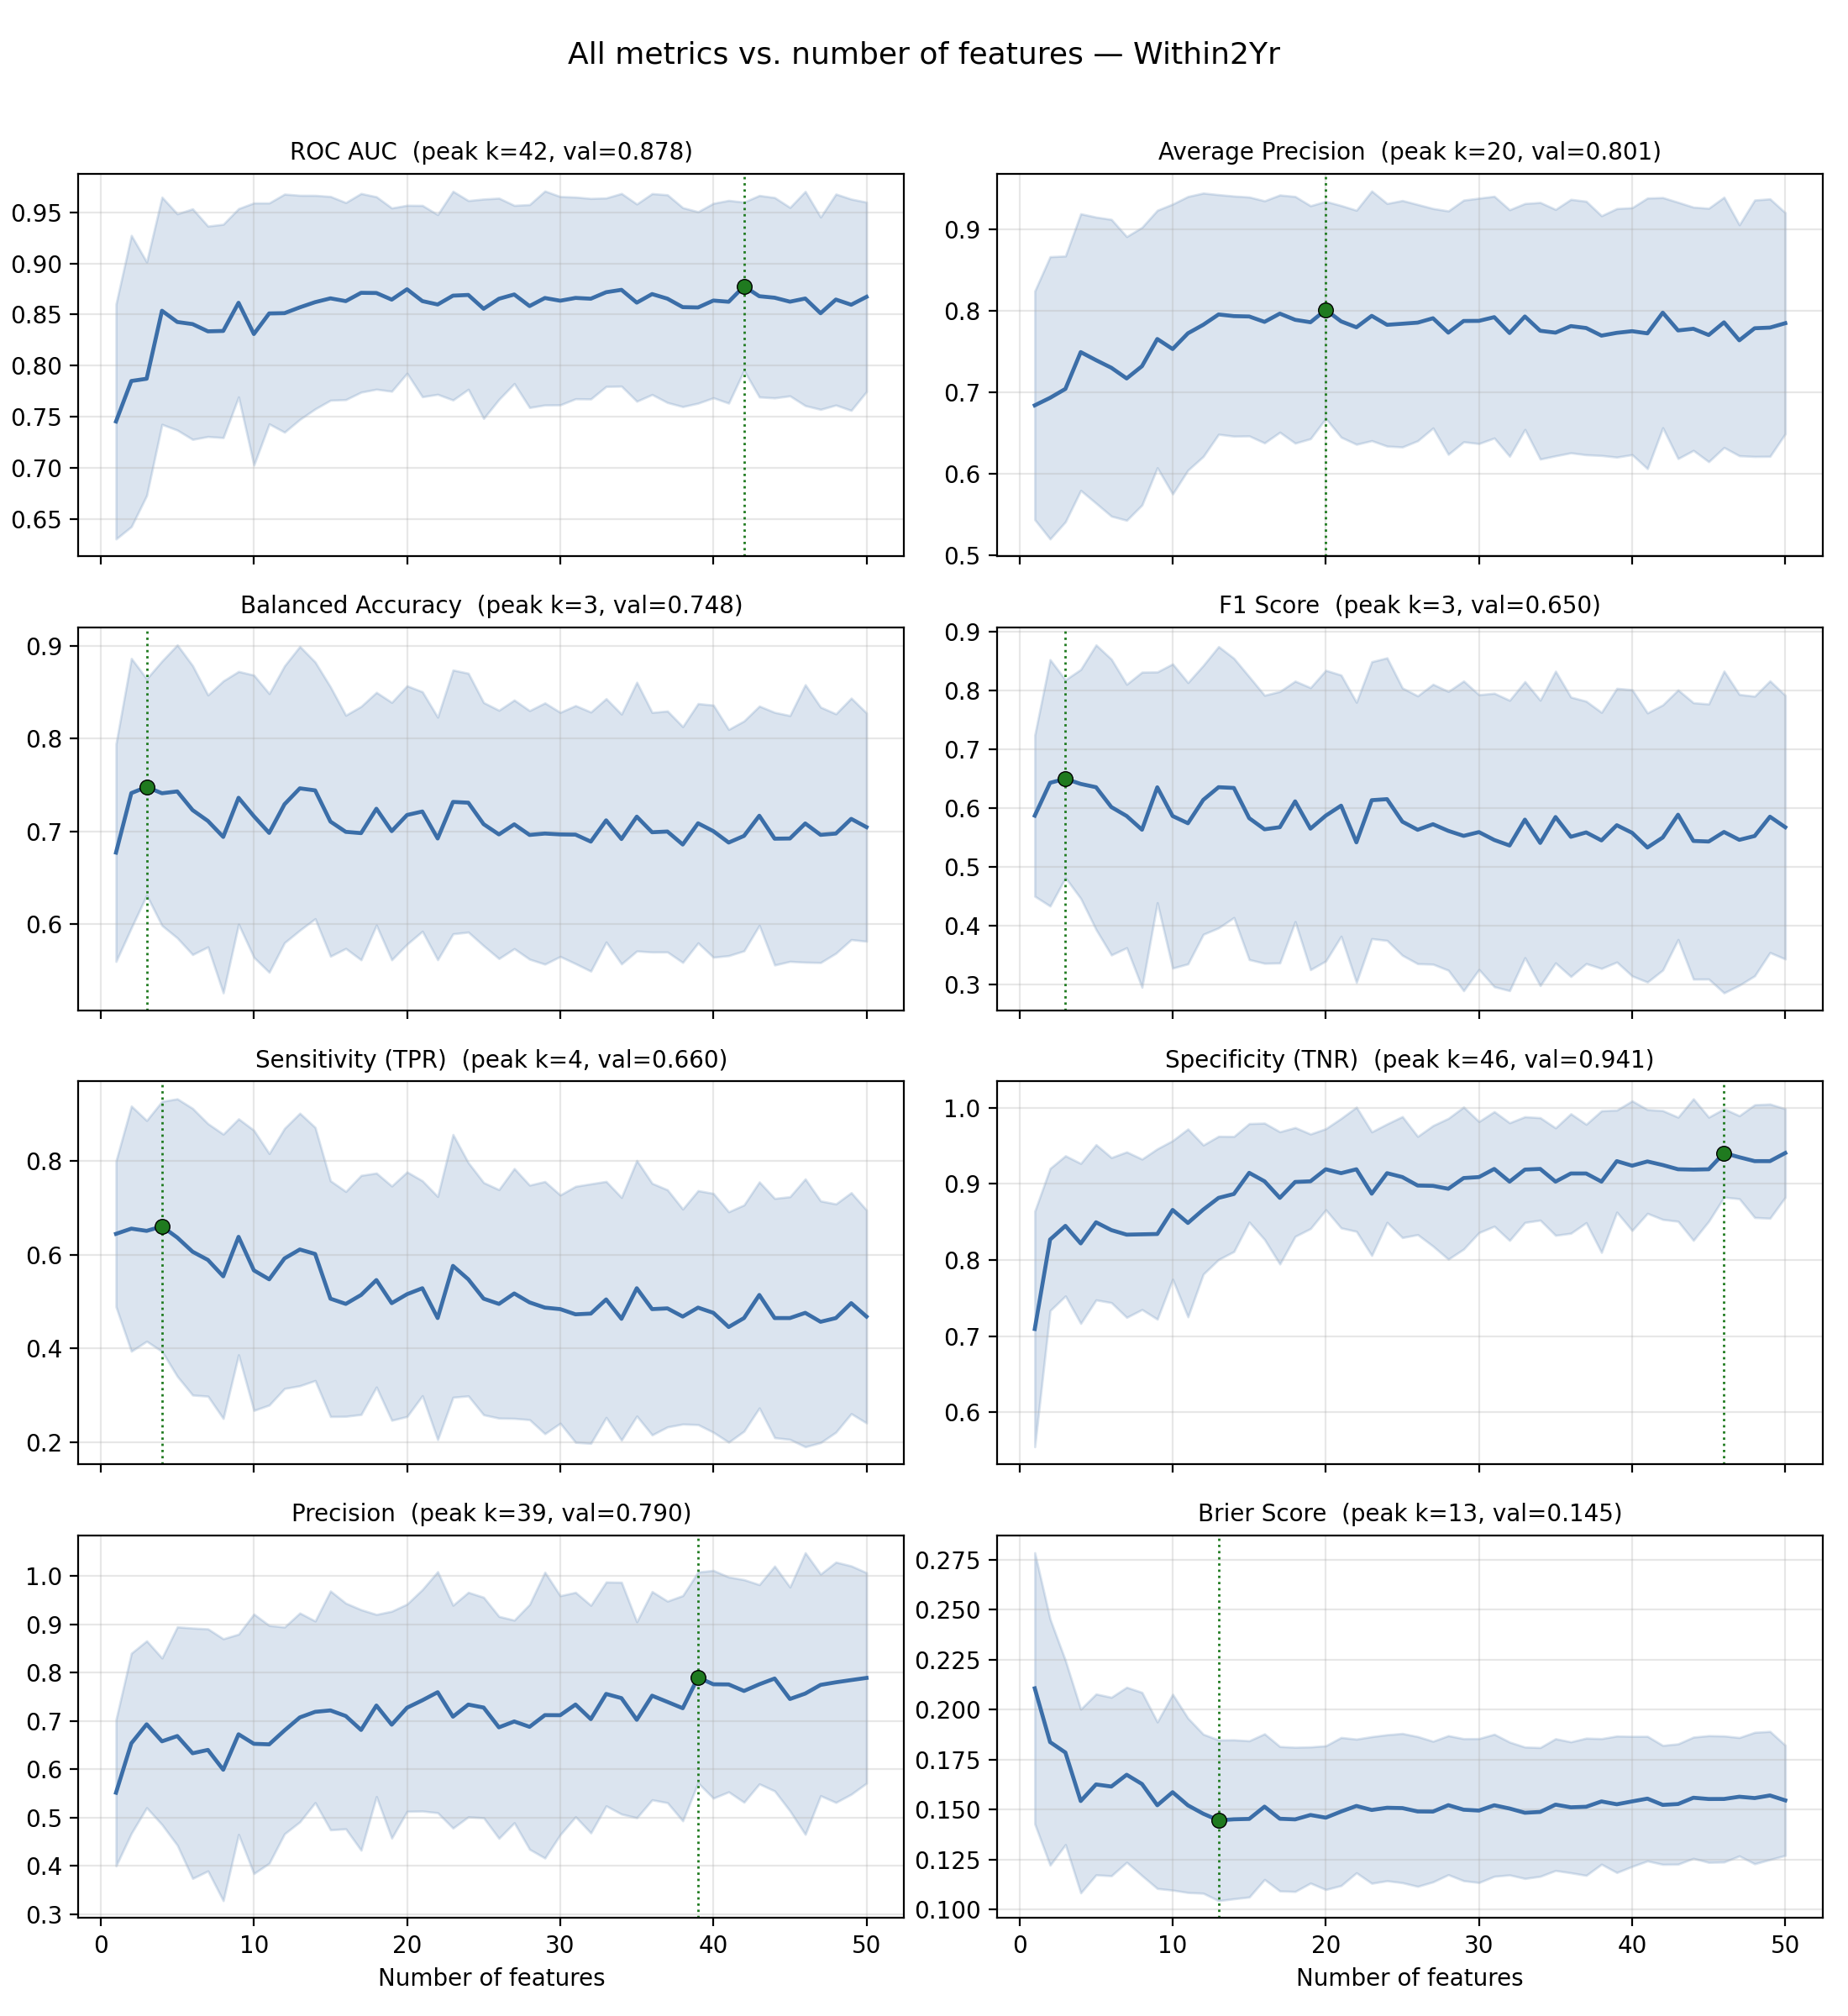
\includegraphics[width=\linewidth]{gradual_allmetrics_within2yr.png}\\
    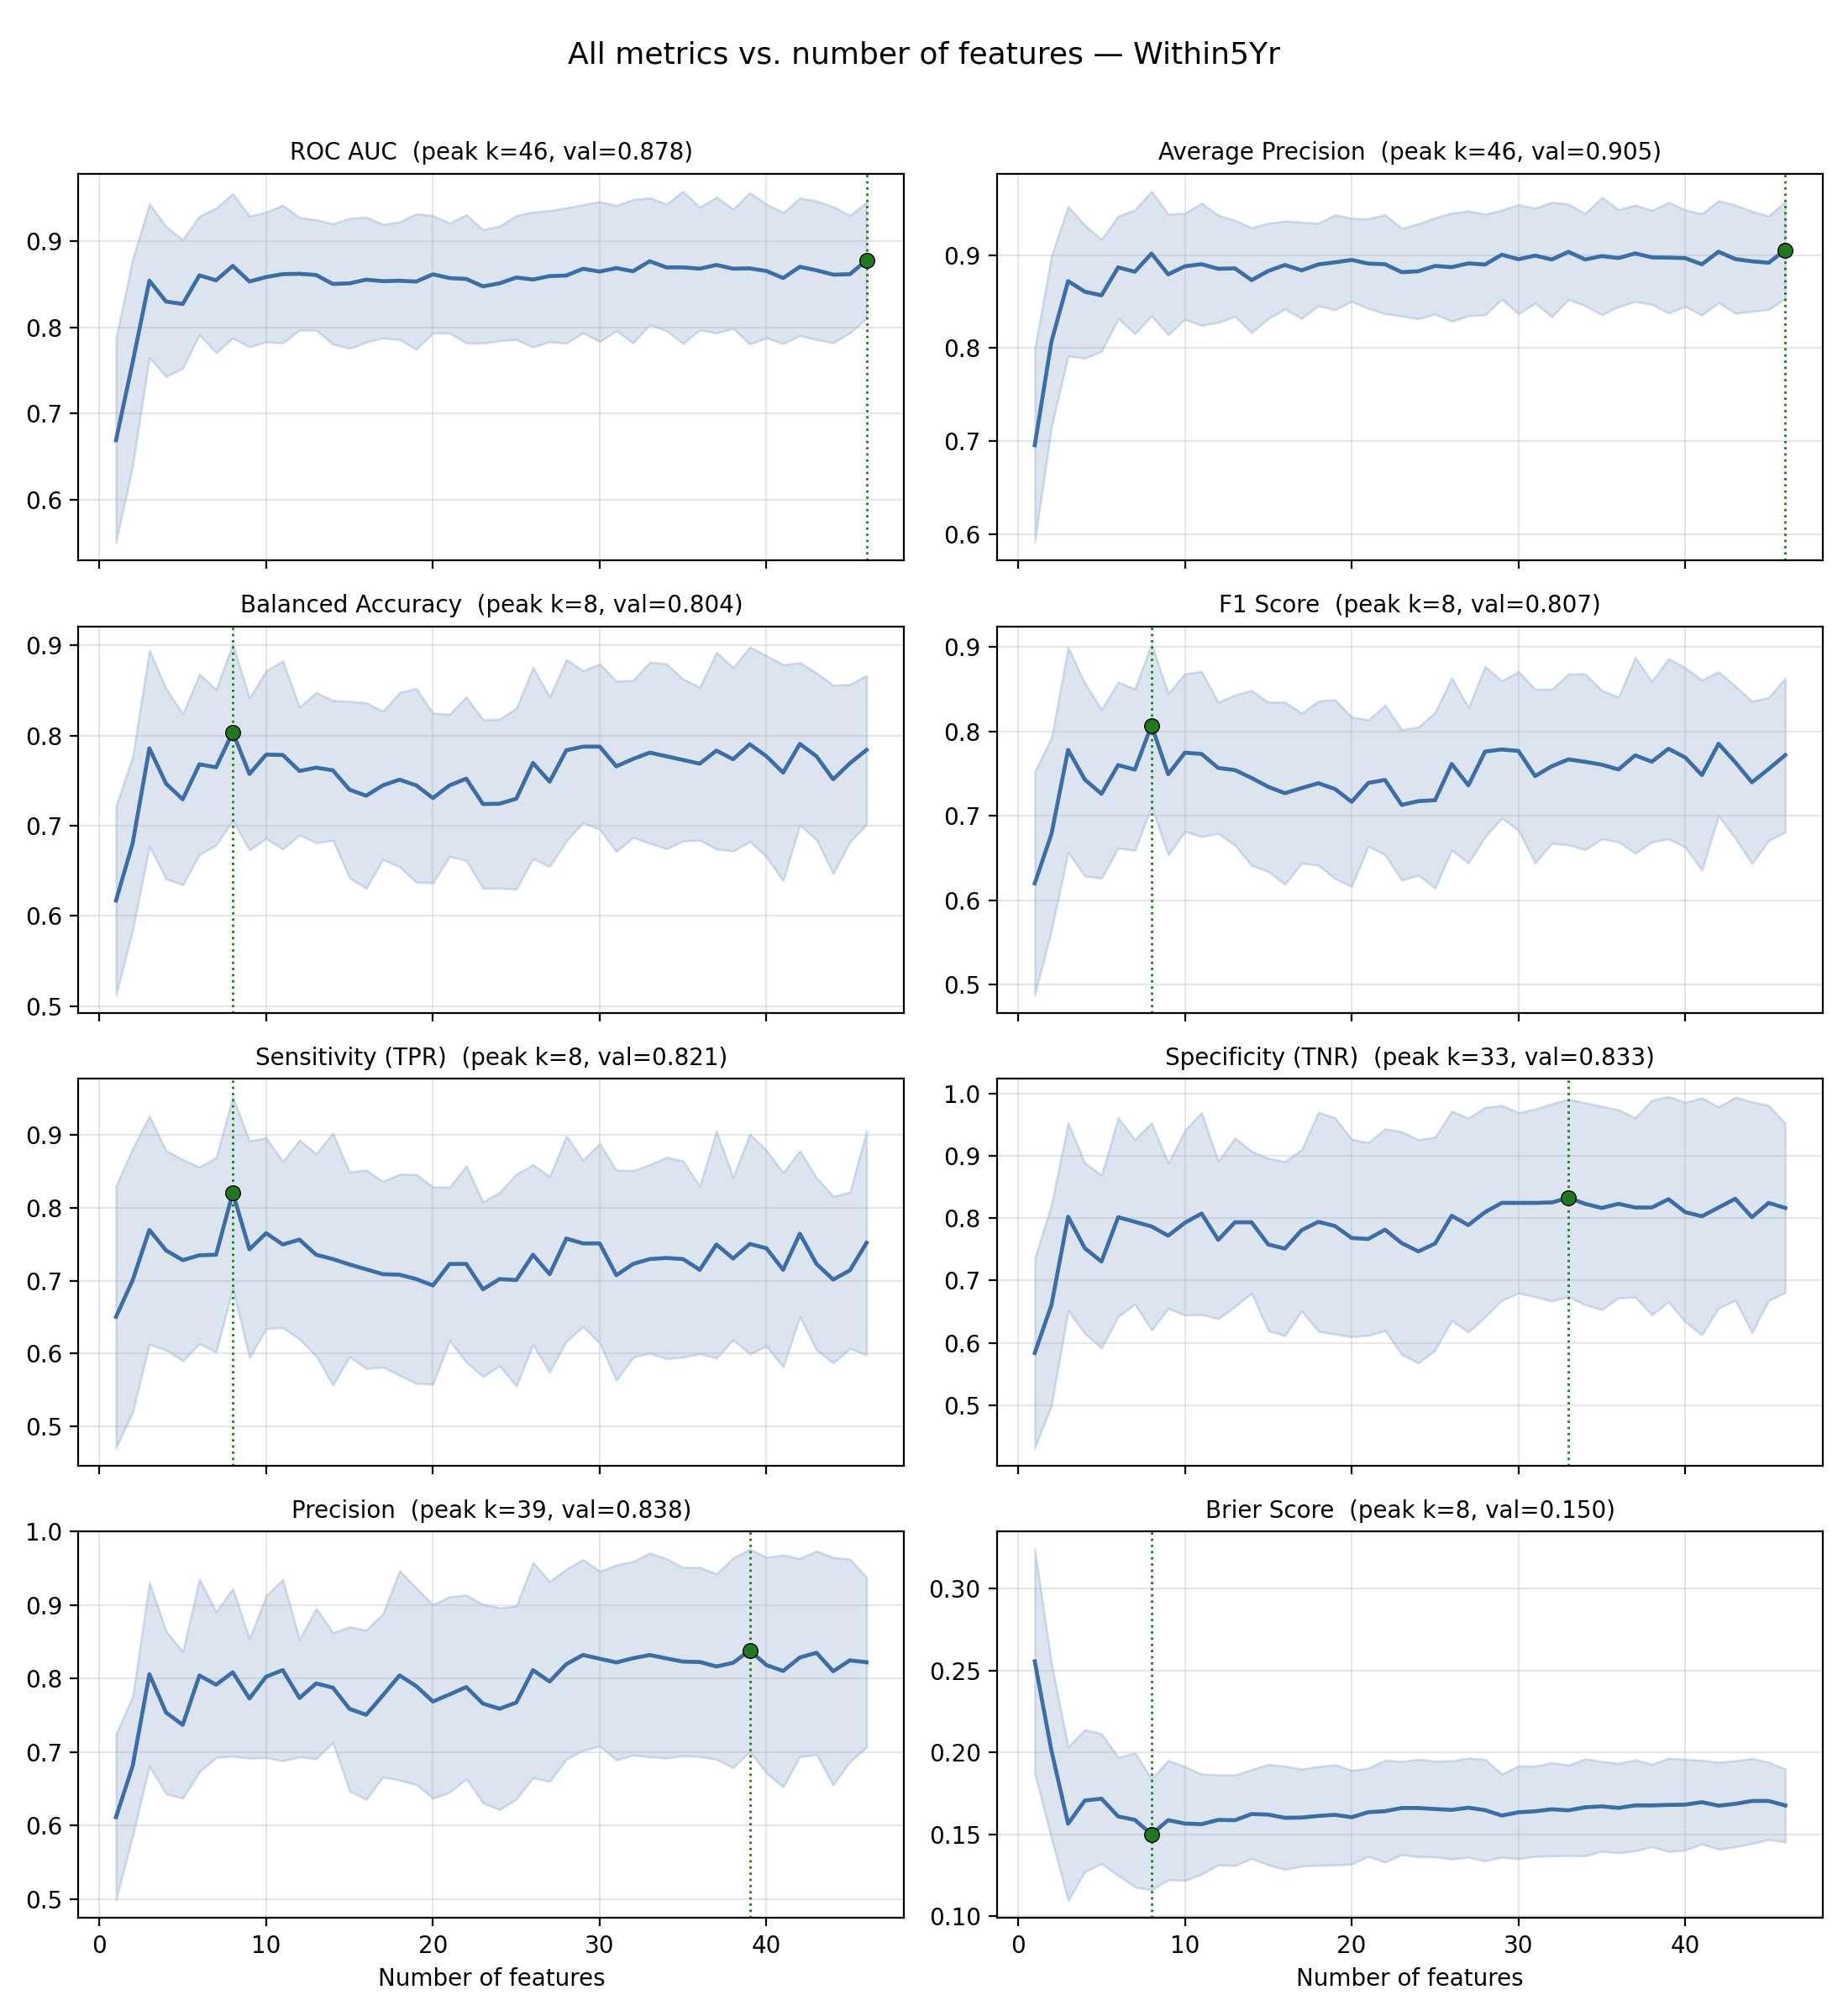
\includegraphics[width=\linewidth]{gradual_allmetrics_within5yr.png}
  \column{0.33\textwidth}
    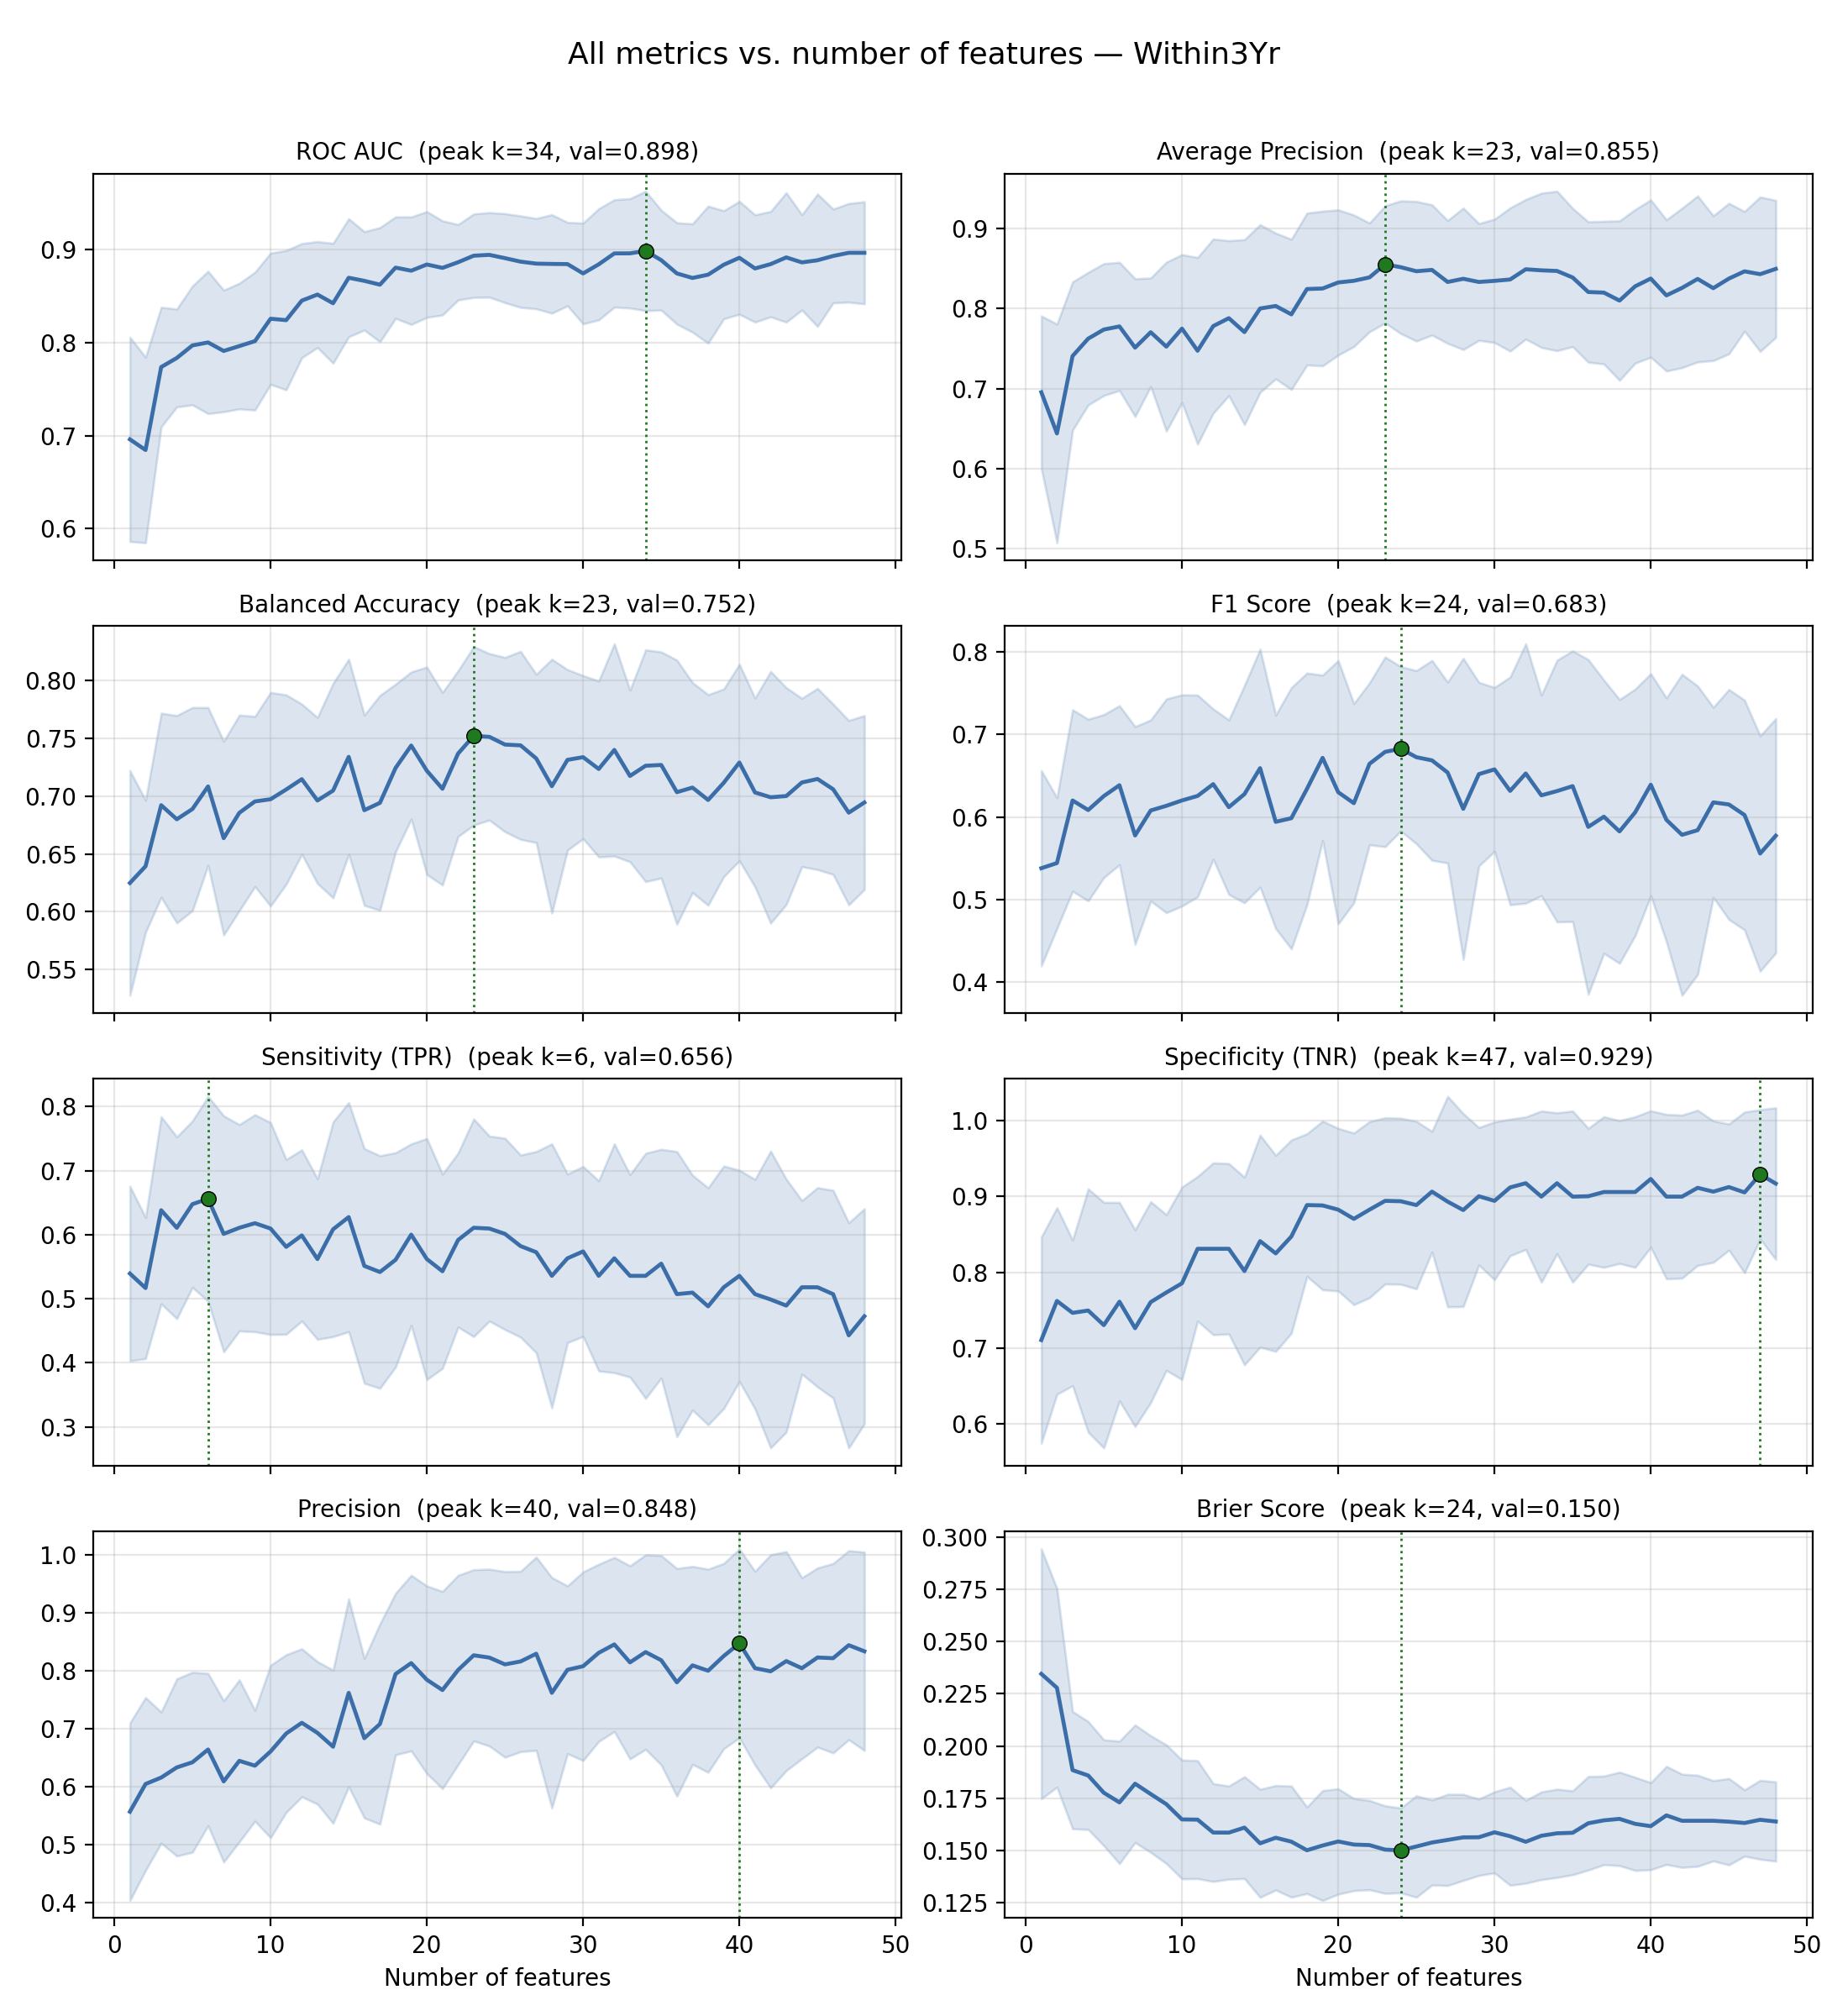
\includegraphics[width=\linewidth]{gradual_allmetrics_within3yr.png}\\
    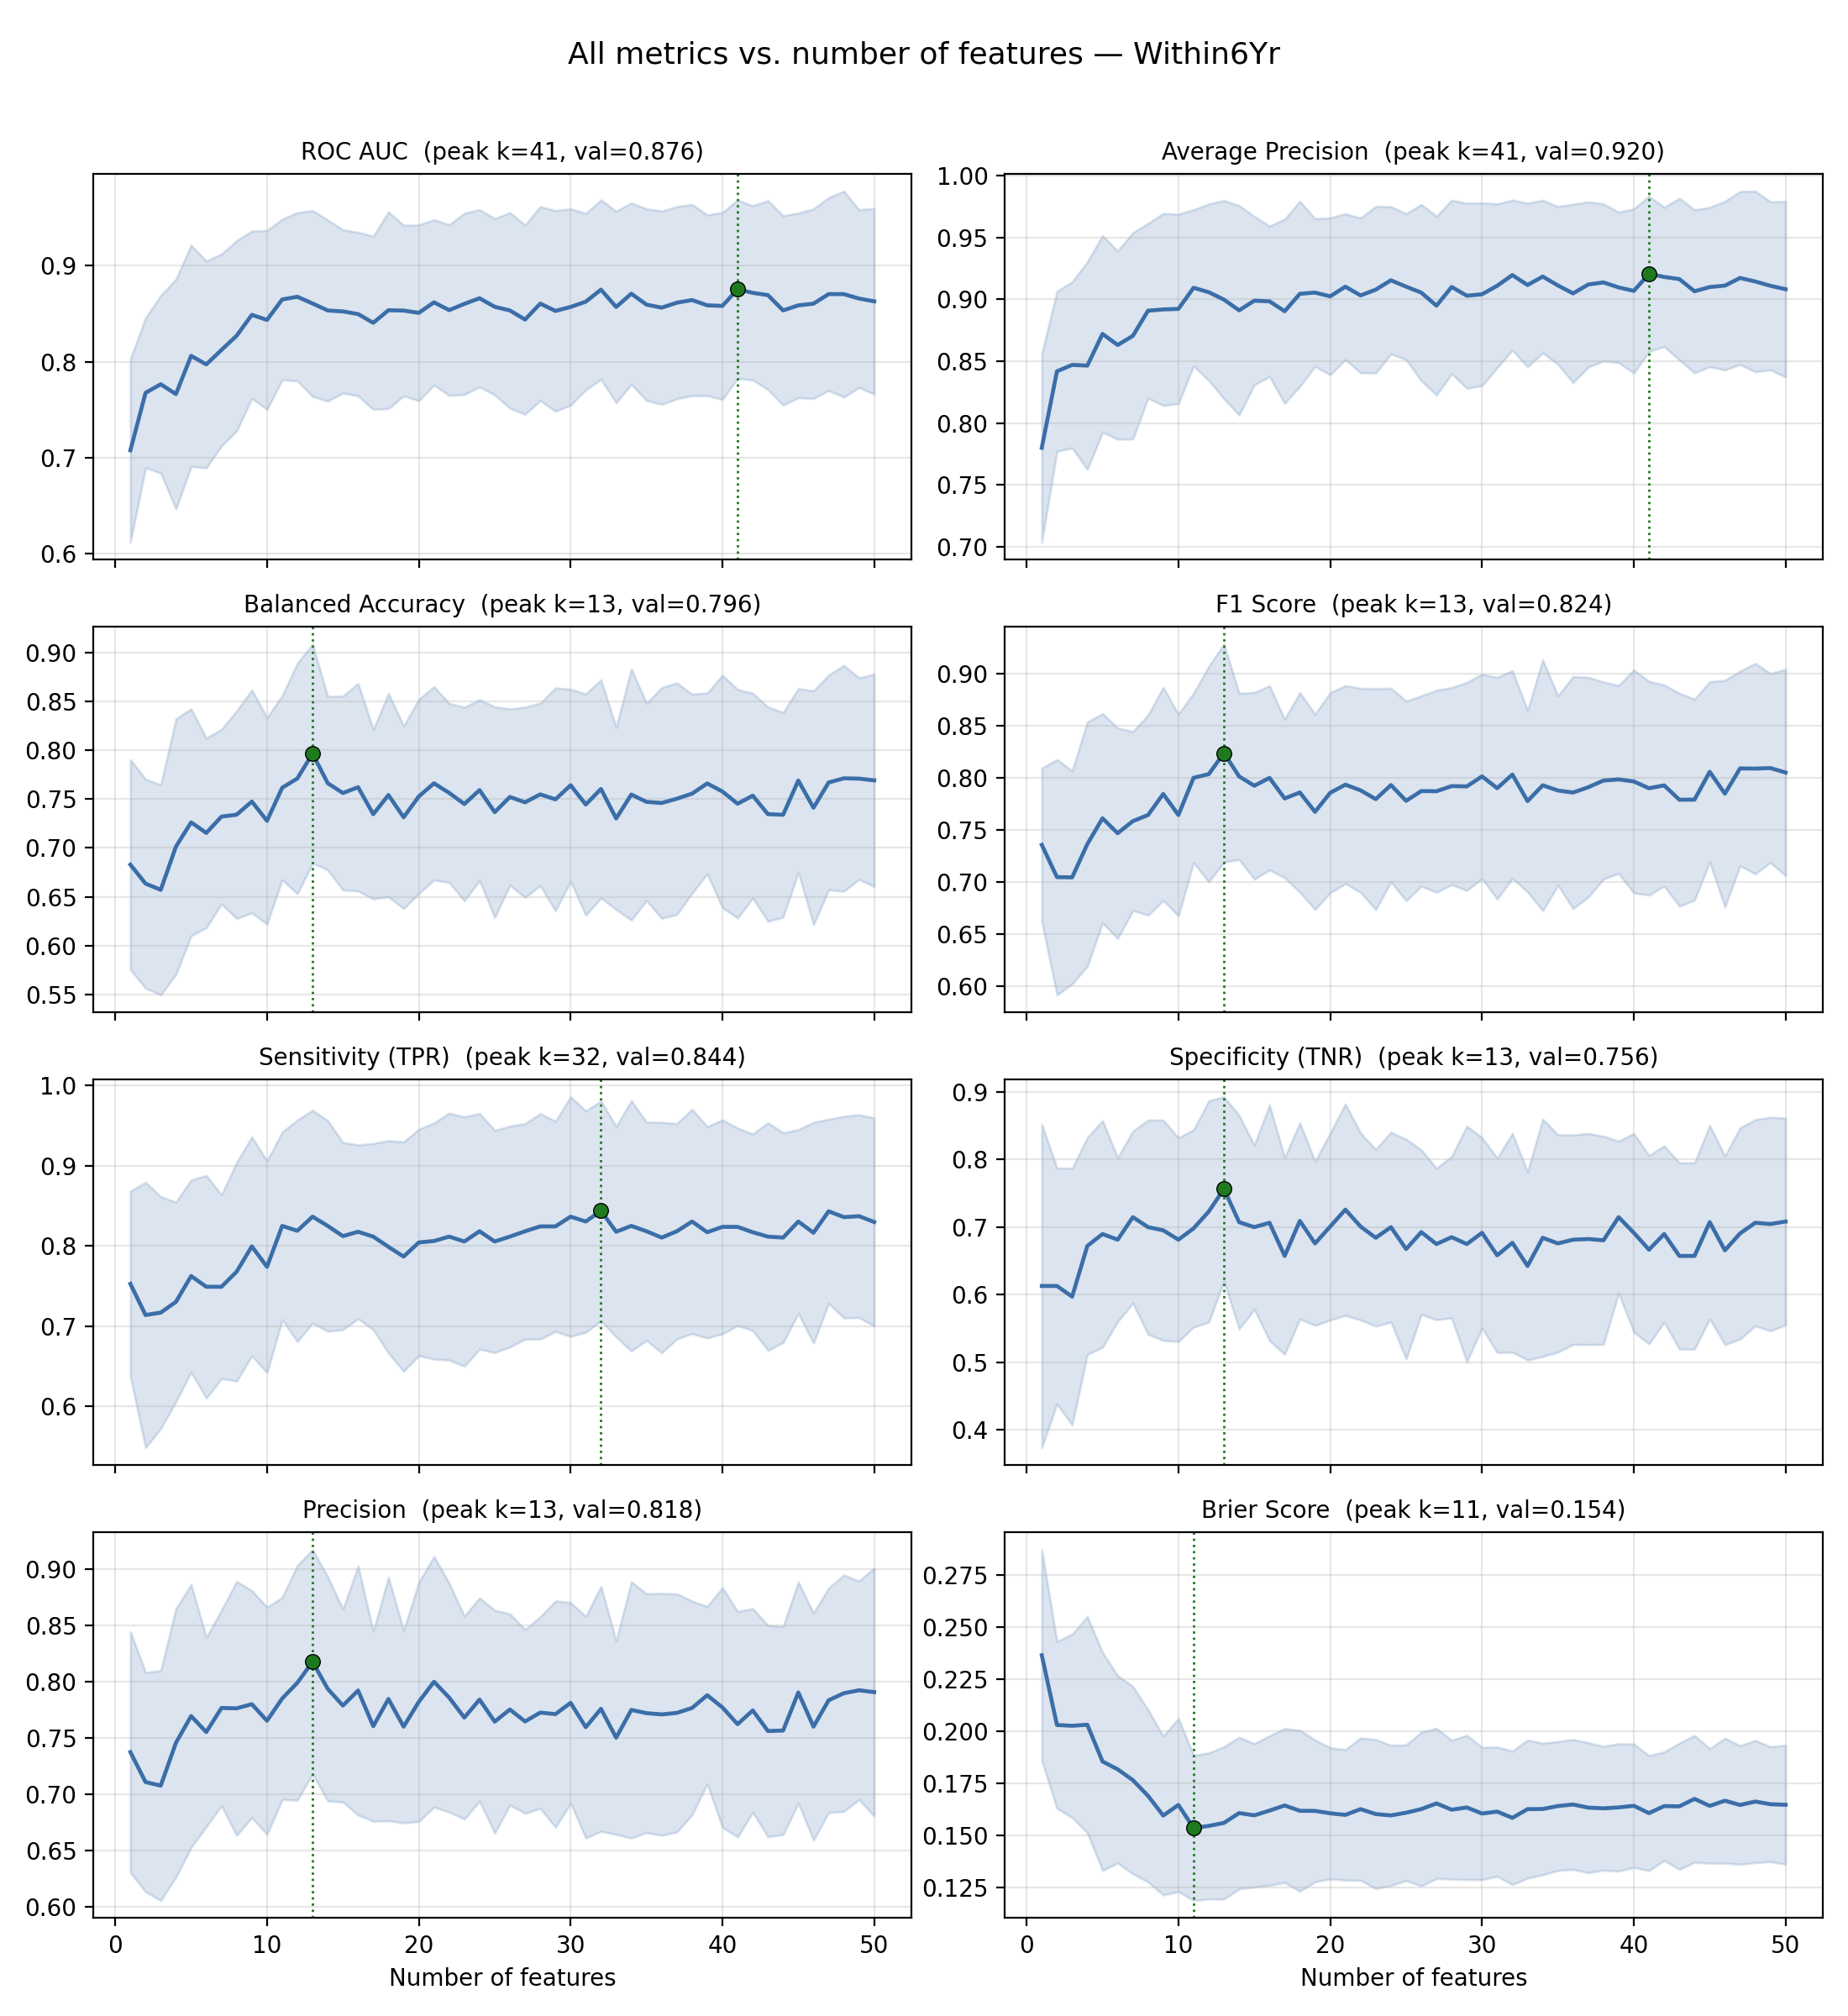
\includegraphics[width=\linewidth]{gradual_allmetrics_within6yr.png}
  \end{columns}
  \scriptsize ``Sharp early gain then plateau'' shape repeats across all six.
\end{frame}

\begin{frame}{Cross-horizon peaks: gradual sweep}
  \begin{figure}
    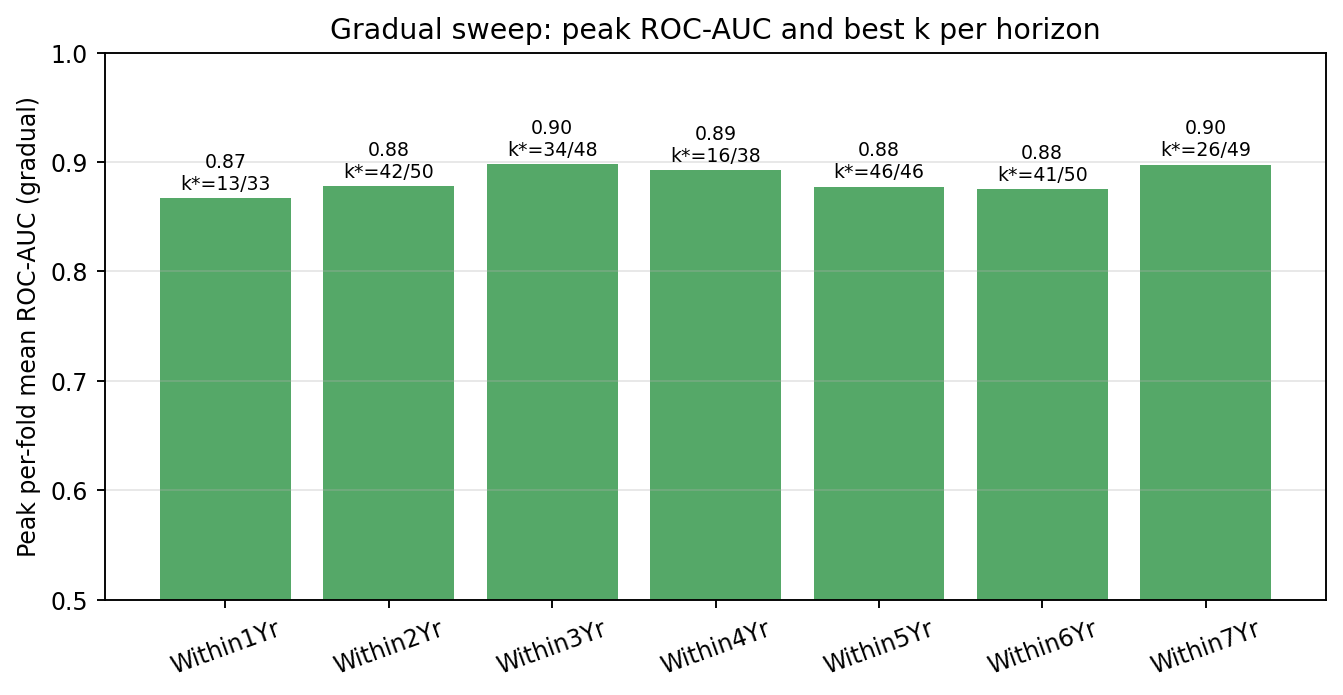
\includegraphics[width=0.78\textwidth]{compare_peakauc_horizons.png}
  \end{figure}
  \begin{itemize}
    \item Peak AUC ranges $0.87$--$0.90$ across all seven horizons.
    \item $k^\star$ is almost always smaller than $|\mathcal{F}|$ --
          parsimony argument (next we zoom into the strongest classifier).
  \end{itemize}
\end{frame}

% =============================================================================
\section{Headline results -- Within7Yr}

\begin{frame}{Within7Yr -- pooled discrimination}
  \begin{columns}[T]
  \column{0.55\textwidth}
    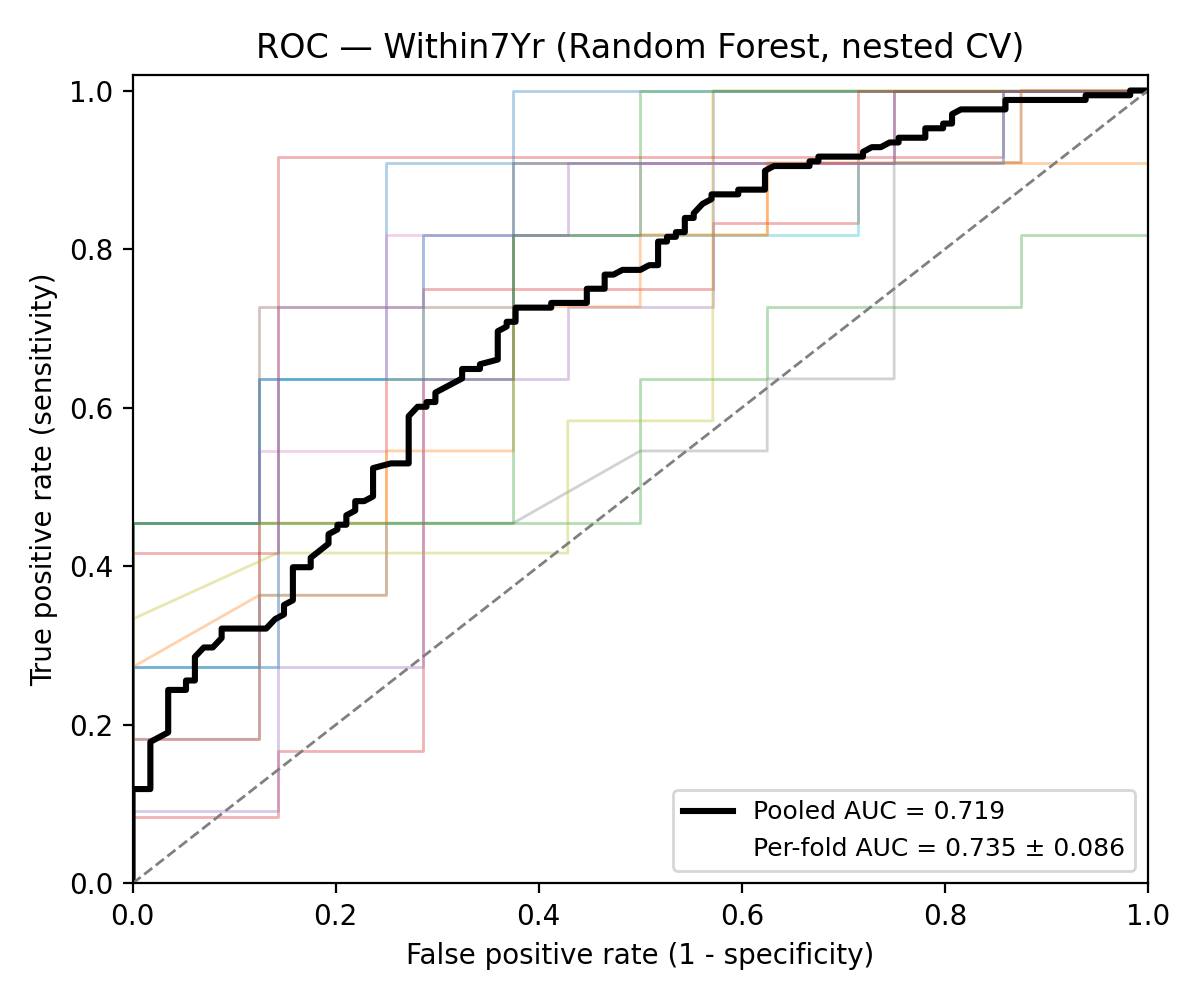
\includegraphics[width=\linewidth]{main_roc_within7yr.png}
  \column{0.45\textwidth}
    \begin{itemize}
      \item Pooled OOF \textbf{ROC-AUC = 0.719}
      \item Per-fold mean AUC $= 0.735 \pm 0.089$
      \item Pooled \textbf{Average Precision = 0.792}
      \item $|\mathcal{F}|=49$ stability-selected features
      \item Best HP:
            \texttt{n\_est=300},
            \texttt{max\_depth=None},
            \texttt{min\_leaf=1},
            \texttt{max\_features=sqrt}.
    \end{itemize}
  \end{columns}
\end{frame}

\begin{frame}{Within7Yr -- operating points}
  \begin{columns}[T]
  \column{0.5\textwidth}
    \begin{figure}
      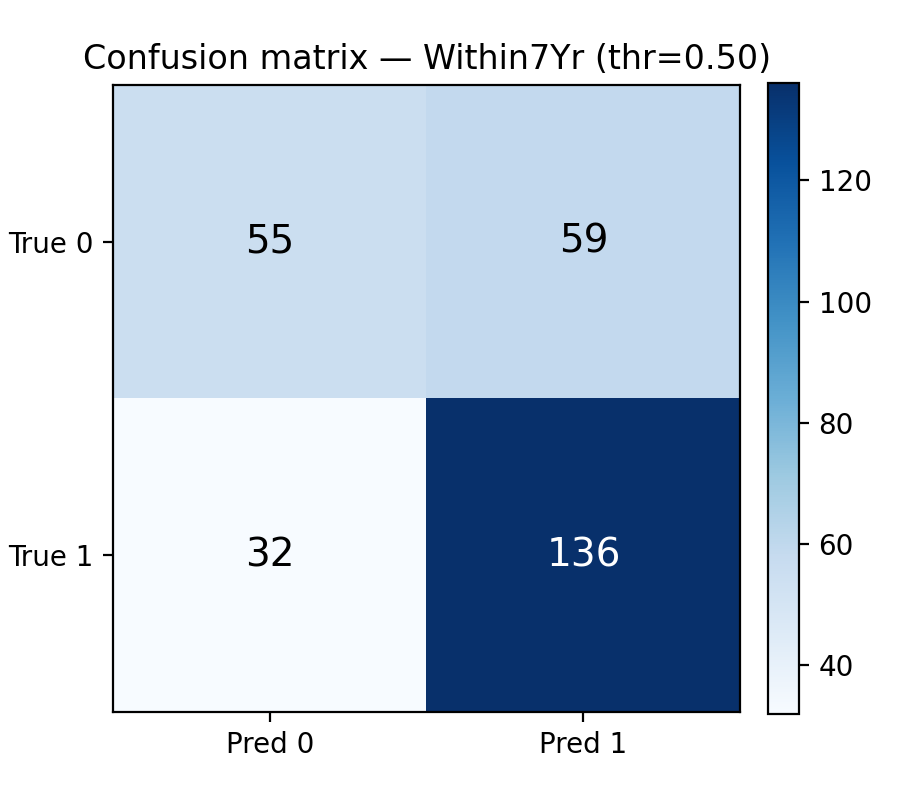
\includegraphics[width=\linewidth]{main_cm05_within7yr.png}
      \caption*{$\tau=0.50$: Sens $0.81$, Spec $0.48$}
    \end{figure}
  \column{0.5\textwidth}
    \begin{figure}
      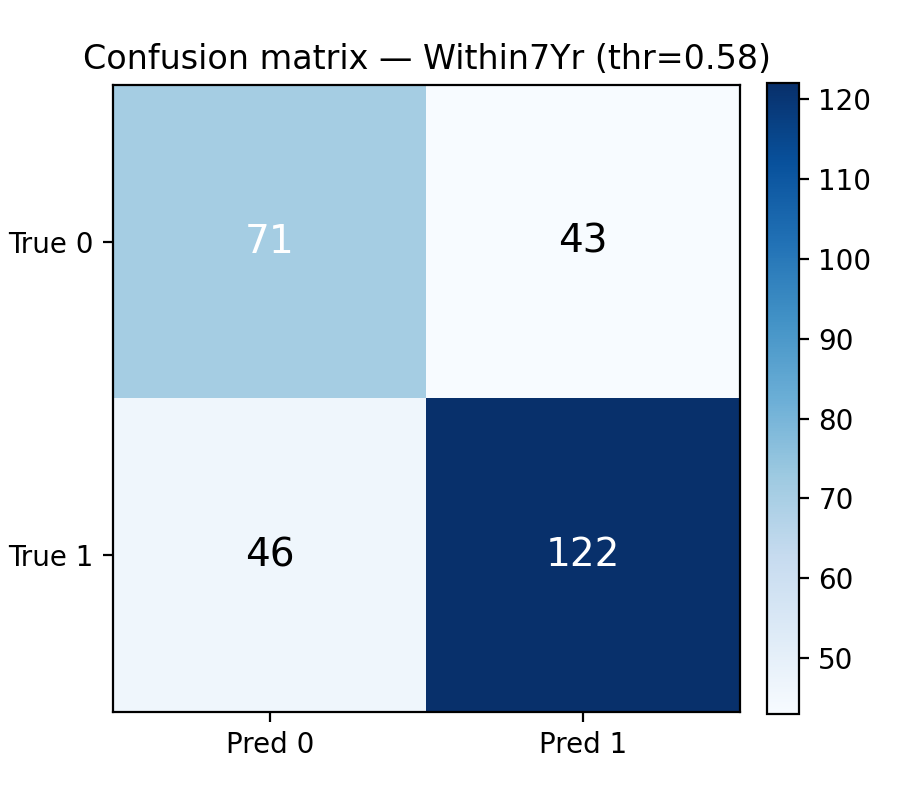
\includegraphics[width=\linewidth]{main_cmyouden_within7yr.png}
      \caption*{Youden $\tau^\star=0.58$: Sens $0.73$, Spec $0.62$}
    \end{figure}
  \end{columns}
  \begin{itemize}
    \item Default $\tau=0.50$ favours sensitivity (catches MACE patients,
          many false alarms).
    \item Youden cut rebalances: \textbf{balanced accuracy $0.674$},
          recommended for clinical use.
  \end{itemize}
\end{frame}

\begin{frame}{Within7Yr -- which features matter?}
  \begin{columns}[T]
  \column{0.5\textwidth}
    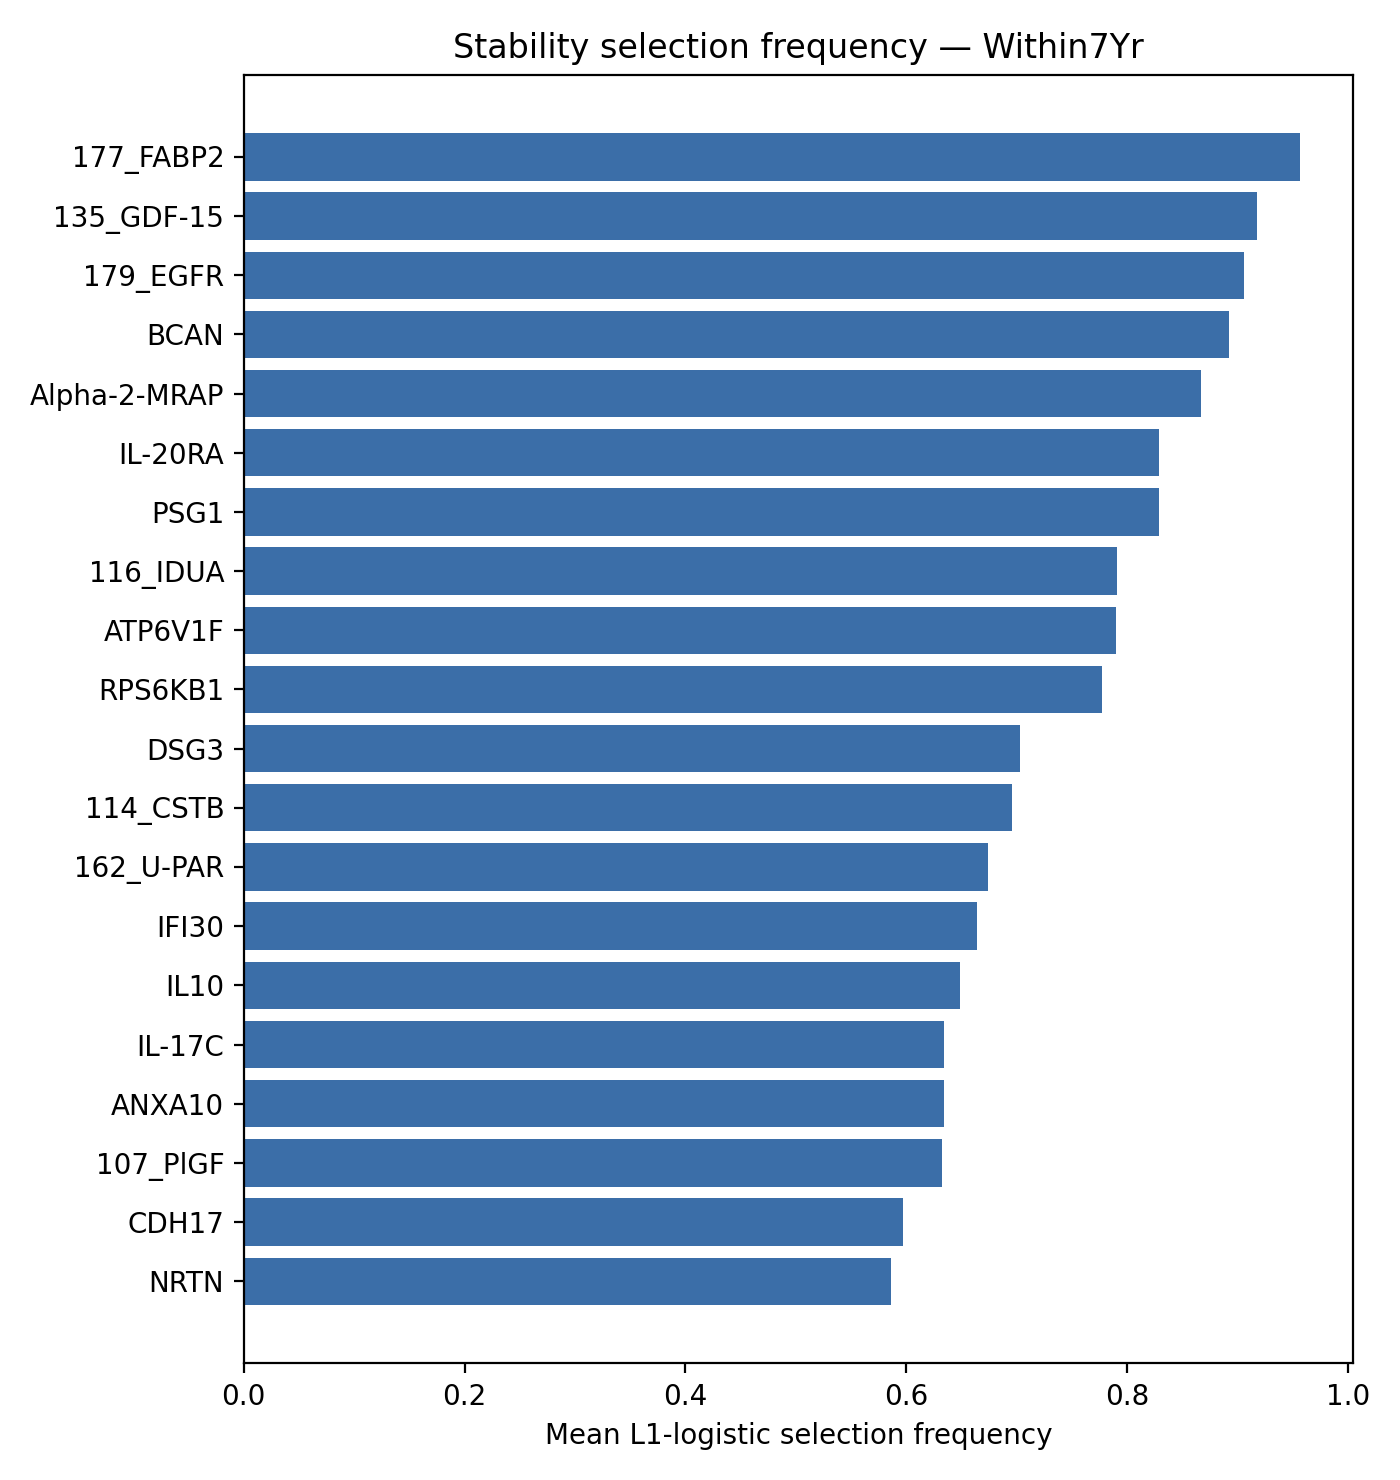
\includegraphics[width=\linewidth]{main_stability_within7yr.png}
    \begin{center}\scriptsize Stability-selection frequency\end{center}
  \column{0.5\textwidth}
    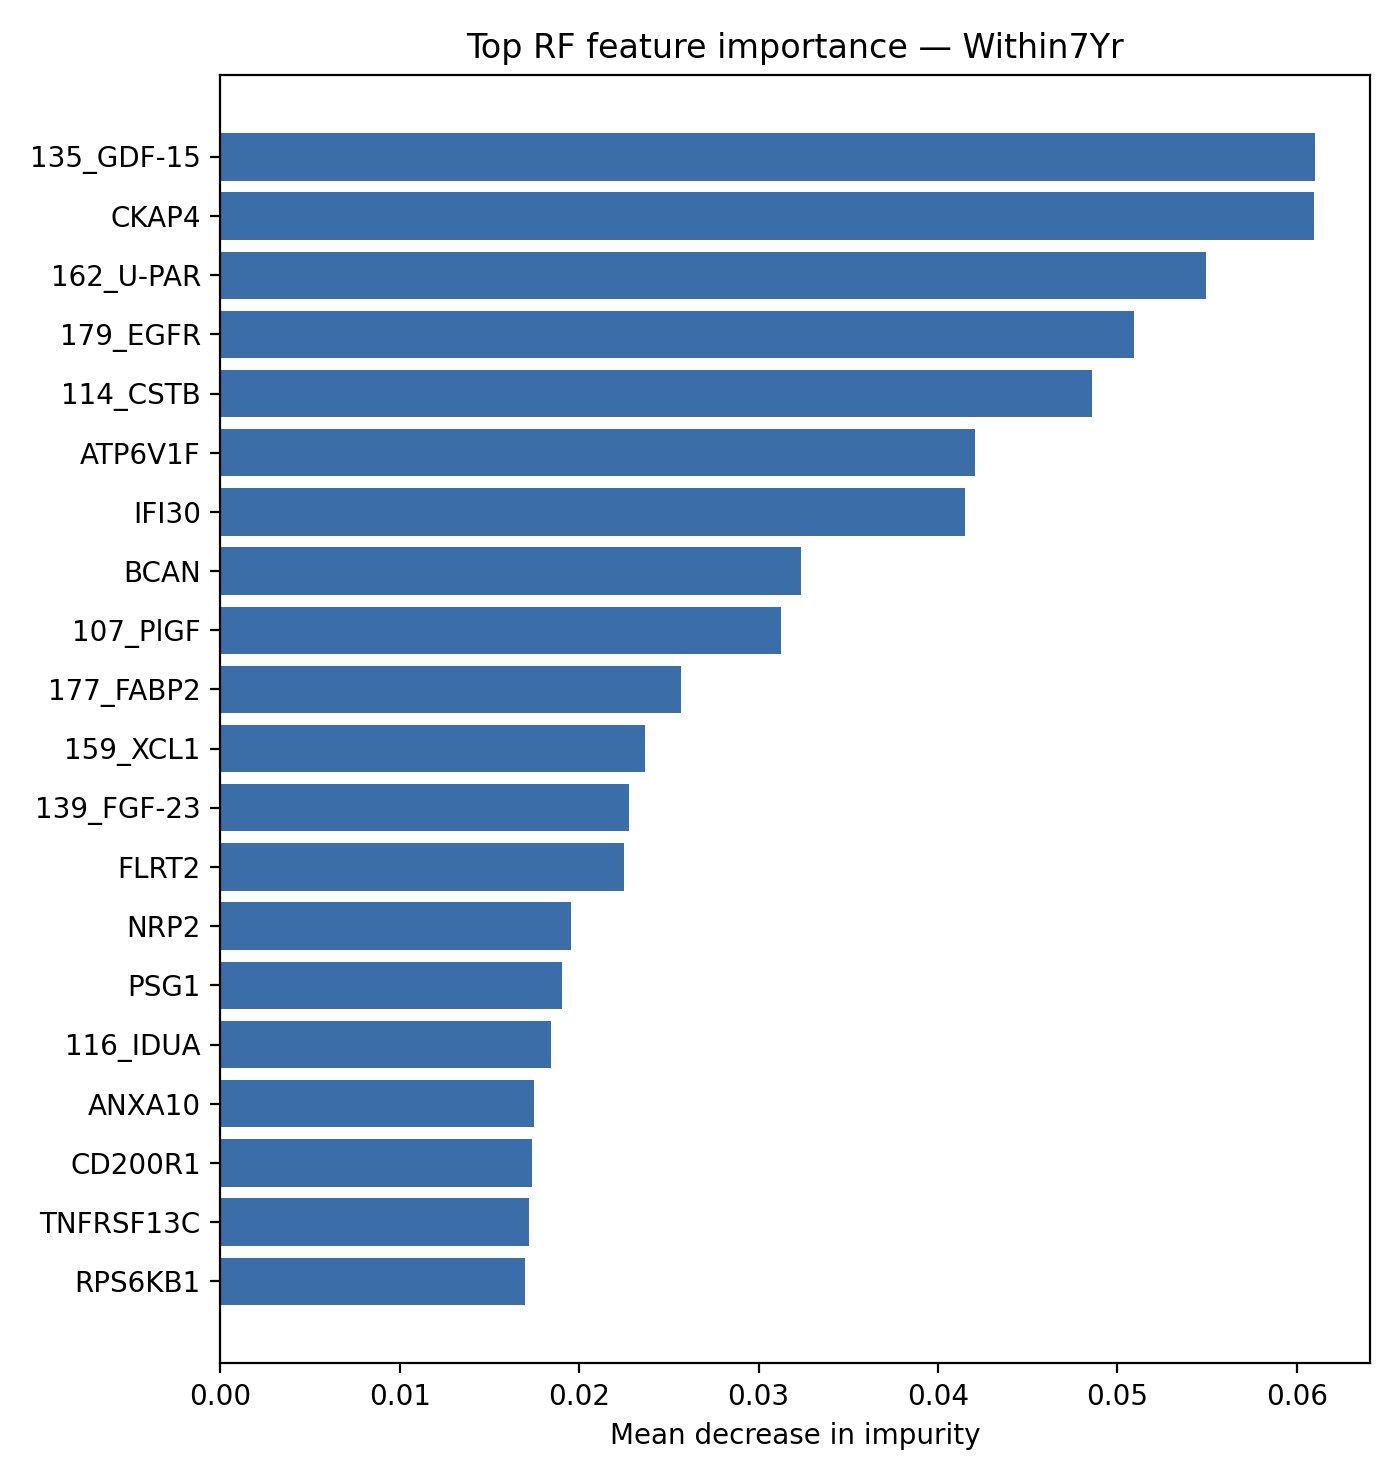
\includegraphics[width=\linewidth]{main_rfimp_within7yr.png}
    \begin{center}\scriptsize Random-Forest impurity importance\end{center}
  \end{columns}
  \vspace{0.3em}
  \begin{itemize}
    \item Always-selected: \texttt{ATP6V1F}, \texttt{179\_EGFR},
          \texttt{135\_GDF-15}, \texttt{BCAN}, \texttt{IL-20RA},
          \texttt{177\_FABP2}.
    \item Top RF importance: \texttt{135\_GDF-15}, \texttt{CKAP4},
          \texttt{162\_U-PAR}, \texttt{179\_EGFR}, \texttt{114\_CSTB}.
  \end{itemize}
\end{frame}

% =============================================================================
\section{Gradual training -- how many features do we need?}

\begin{frame}{The parsimony question}
  \begin{block}{Idea (one ranking per family)}
    For each of the four families, walk down \emph{that family's}
    published feature ranking (\texttt{rf\_importance},
    \texttt{xgb\_importance}, \texttt{lr\_importance},
    \texttt{svm\_importance}). At every truncation
    $k=1,2,\dots,|\mathcal{F}|$, re-run the same nested CV. Where does
    the curve peak?
  \end{block}
  \begin{itemize}
    \item Same outer/inner CV, same hyperparameter grid as the main pipeline.
    \item Curve $k \mapsto \mathrm{metric}$ is a held-out estimate
          (the \emph{model} at every $k$ is fit fold-respecting).
    \item \textbf{Caveat:} the ranking itself is computed once on the
          full data $\Rightarrow$ small look-ahead. Mild for tree
          importances, much larger for linear / kernel ones (next slide).
  \end{itemize}
\end{frame}

\begin{frame}{Within7Yr -- ten metrics vs $k$}
  \begin{figure}
    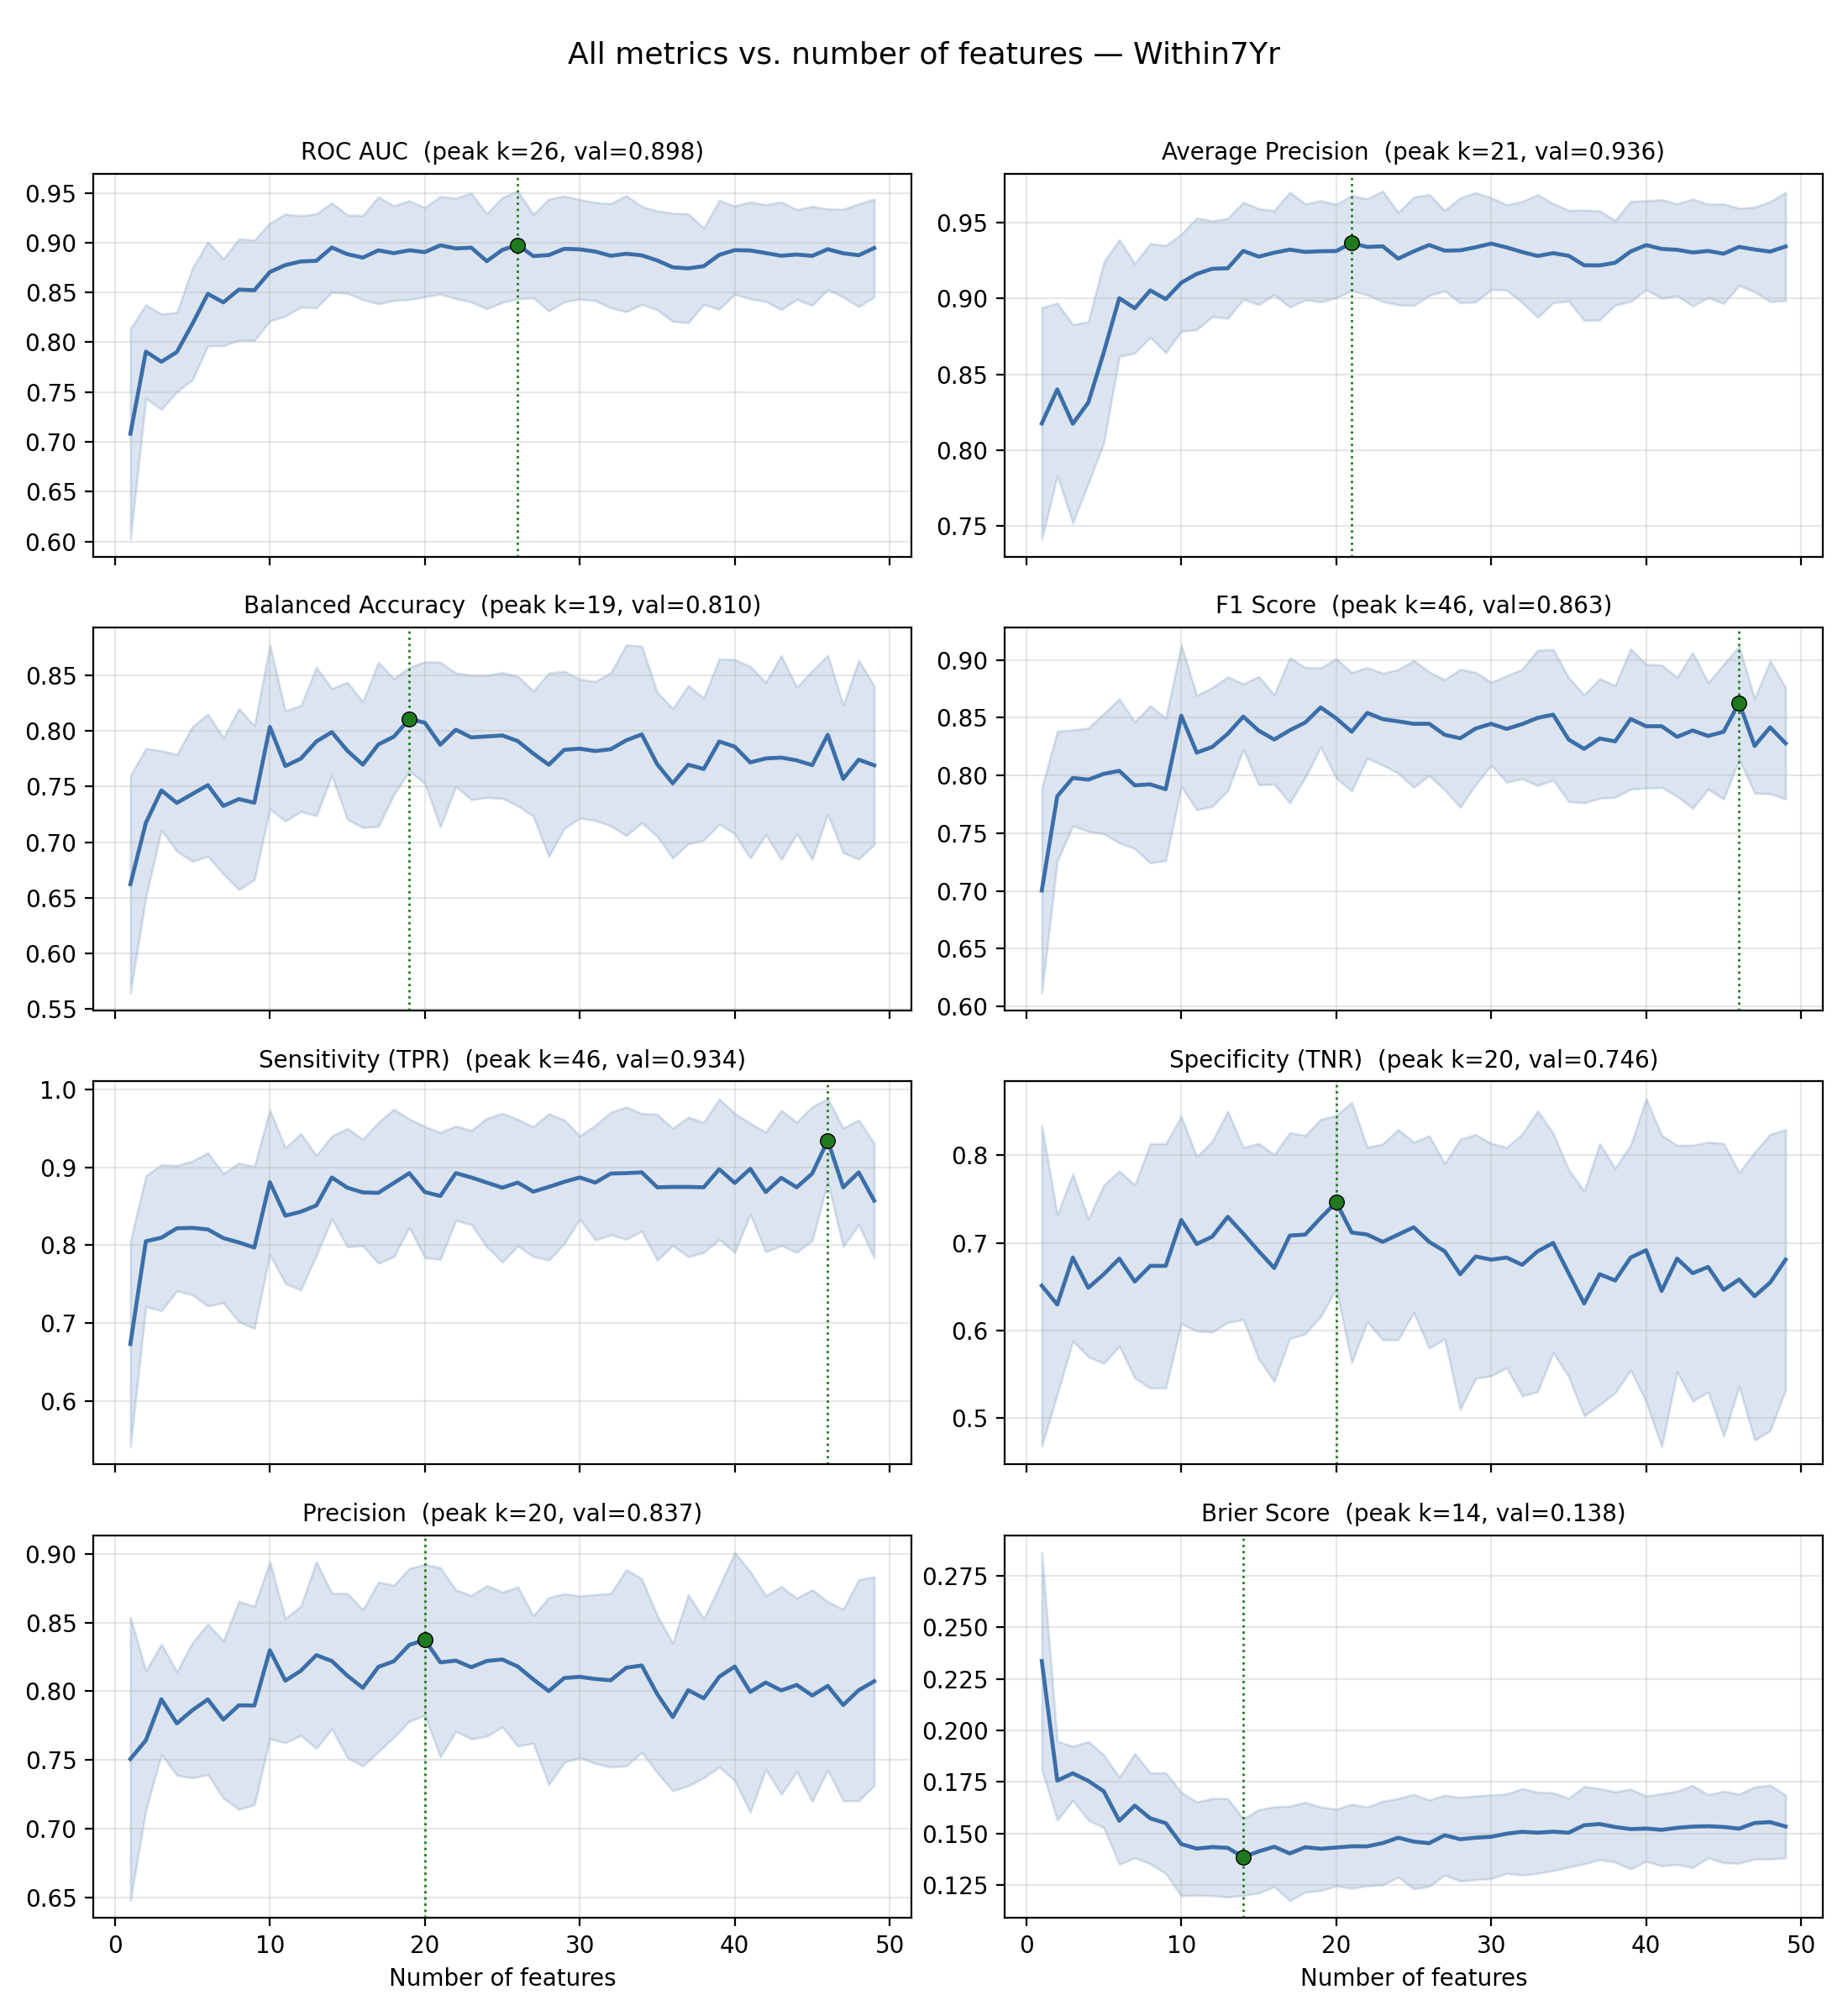
\includegraphics[width=0.95\textwidth]{gradual_allmetrics_within7yr.png}
  \end{figure}
  \begin{itemize}
    \item Discrimination metrics: sharp rise over first 5--10 features.
    \item Plateau / single peak in the band $k\!\in\![14, 26]$.
    \item Long tail of the ranking adds variance, not signal.
  \end{itemize}
\end{frame}

\begin{frame}{Within7Yr -- per-metric peaks (visual)}
  \begin{center}
    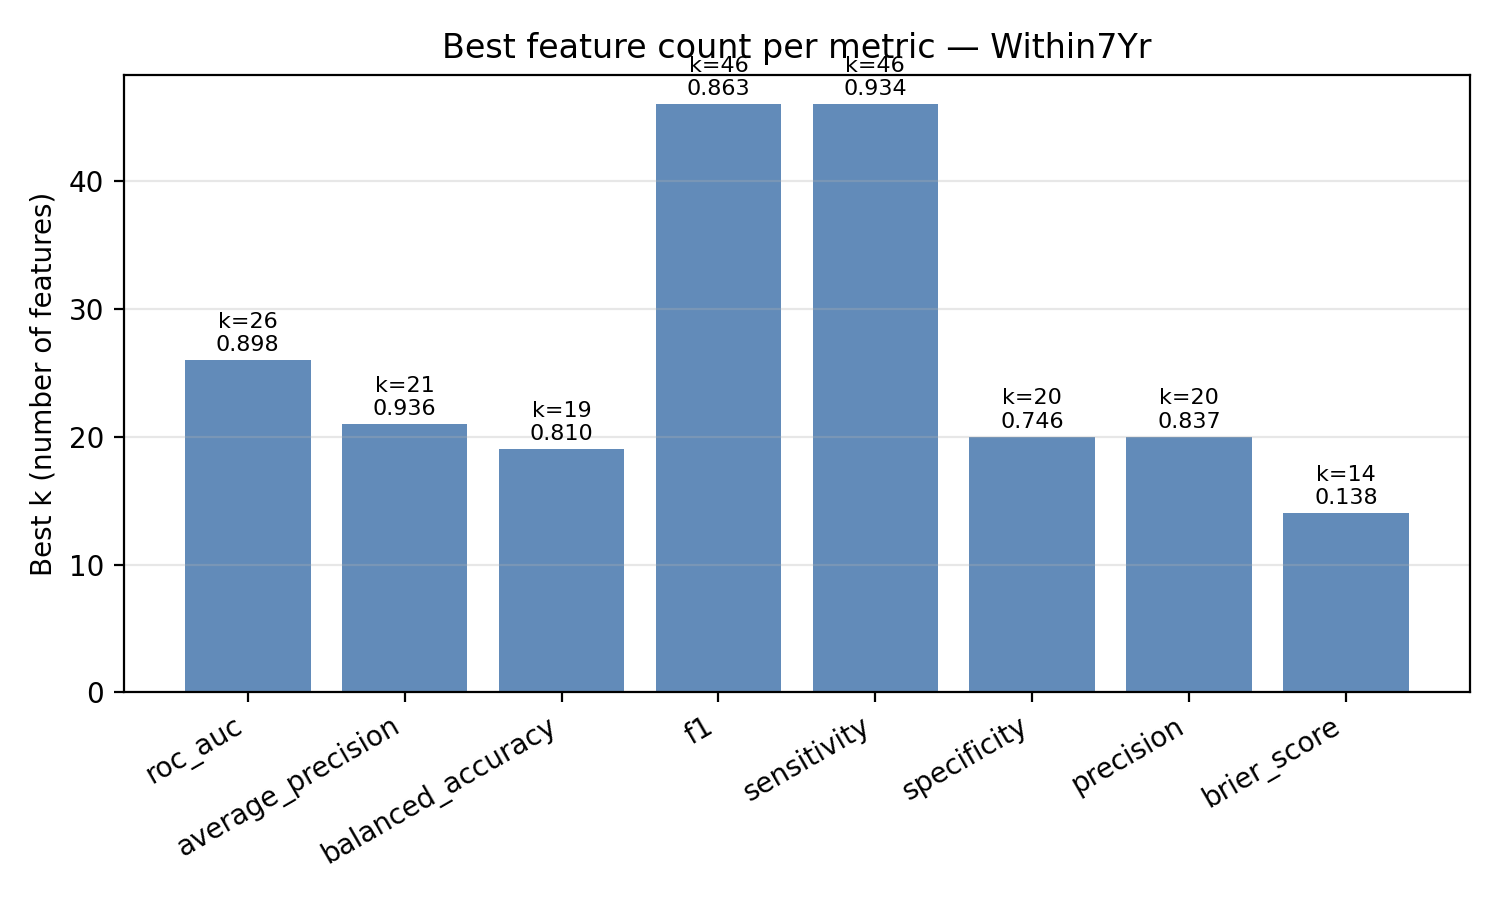
\includegraphics[height=0.78\textheight,keepaspectratio]{gradual_peakmarker_within7yr.png}
  \end{center}
  \scriptsize Each row is one metric; marker at the $k$ that optimises it.
\end{frame}

\begin{frame}{Within7Yr -- per-metric peaks (table)}
  \centering
  \small
  \begin{tabular}{lrcc}
    \toprule
    Metric & Best $k$ & Per-fold mean $\pm$ SD & Pooled OOF \\
    \midrule
    ROC-AUC            & 26 & $0.898 \pm 0.054$ & 0.888 \\
    Average Precision  & 21 & $0.936 \pm 0.031$ & 0.930 \\
    Balanced Accuracy  & 19 & $0.810 \pm 0.046$ & 0.810 \\
    Accuracy           & 19 & $0.826 \pm 0.042$ & 0.826 \\
    F$_1$              & 46 & $0.863 \pm 0.049$ & 0.863 \\
    Sensitivity        & 46 & $0.934 \pm 0.054$ & 0.935 \\
    Specificity        & 20 & $0.746 \pm 0.099$ & 0.746 \\
    Brier (lower better)& 14 & $0.138 \pm 0.019$ & 0.138 \\
    \bottomrule
  \end{tabular}
  \vspace{0.6em}
  \begin{itemize}
    \item Discrimination peaks cluster around $k\!\in\![14, 26]$.
    \item Recall / $F_1$ favour bigger $k$; precision favours $k\!\sim\!20$.
  \end{itemize}
\end{frame}

\begin{frame}{Within7Yr -- ROC at three feature counts}
  \begin{columns}[T]
  \column{0.55\textwidth}
    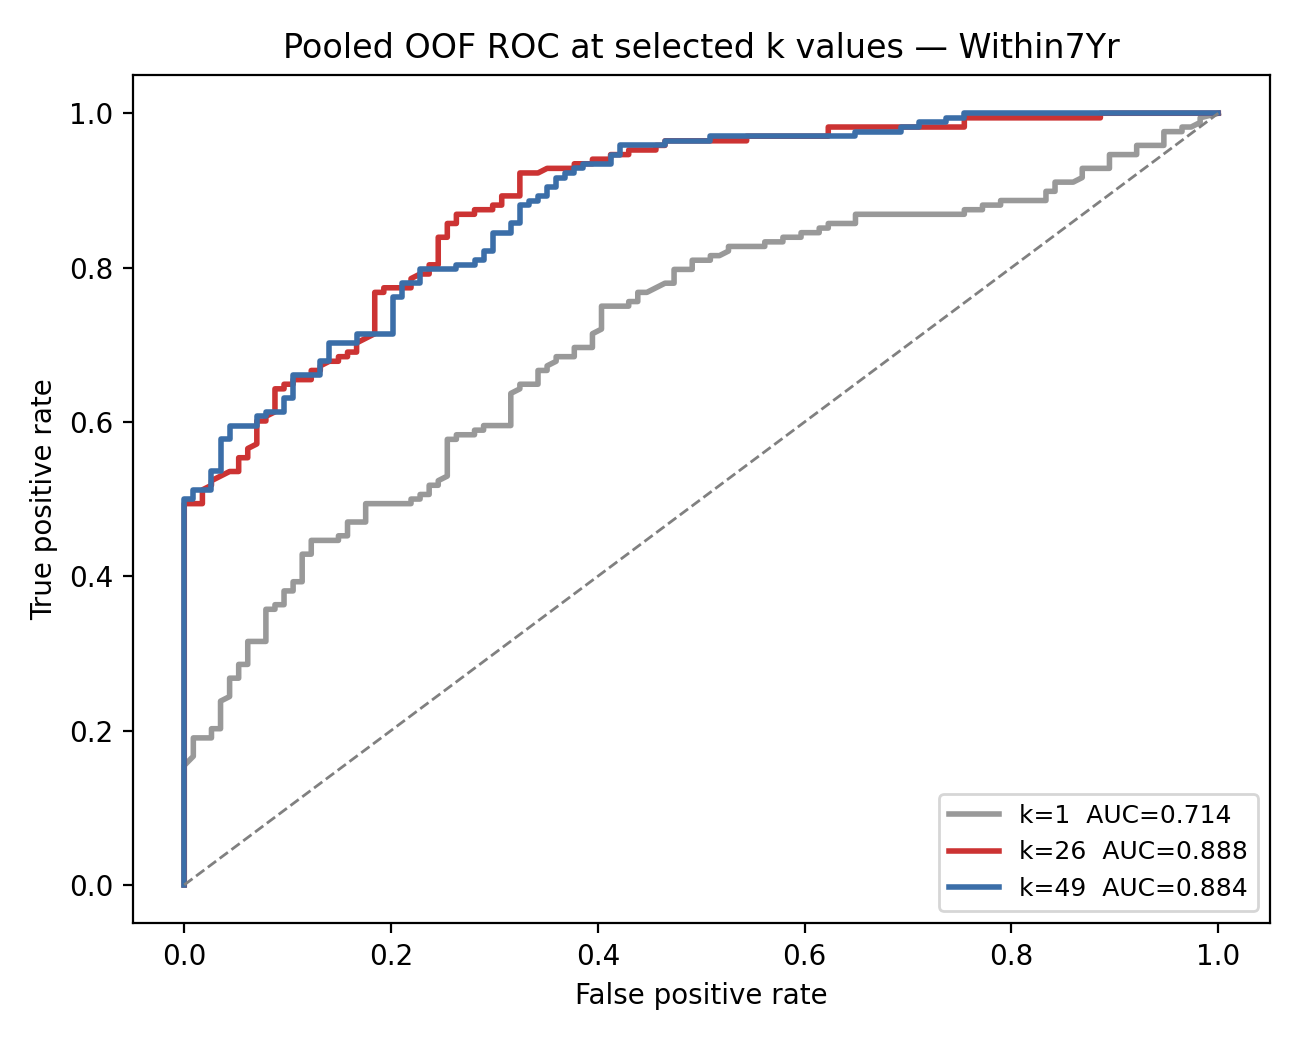
\includegraphics[width=\linewidth]{gradual_roc_within7yr.png}
  \column{0.45\textwidth}
    \begin{itemize}
      \item $k=1$: AUC $\approx 0.66$ -- single biomarker already
            non-trivial.
      \item $k=k^\star$: AUC $= 0.888$ -- peak.
      \item $k=|\mathcal{F}|=49$: AUC $= 0.717$.
      \item Adding the long tail \emph{hurts}.
    \end{itemize}
  \end{columns}
\end{frame}

\begin{frame}{Within7Yr -- per-fold heatmap}
  \begin{figure}
    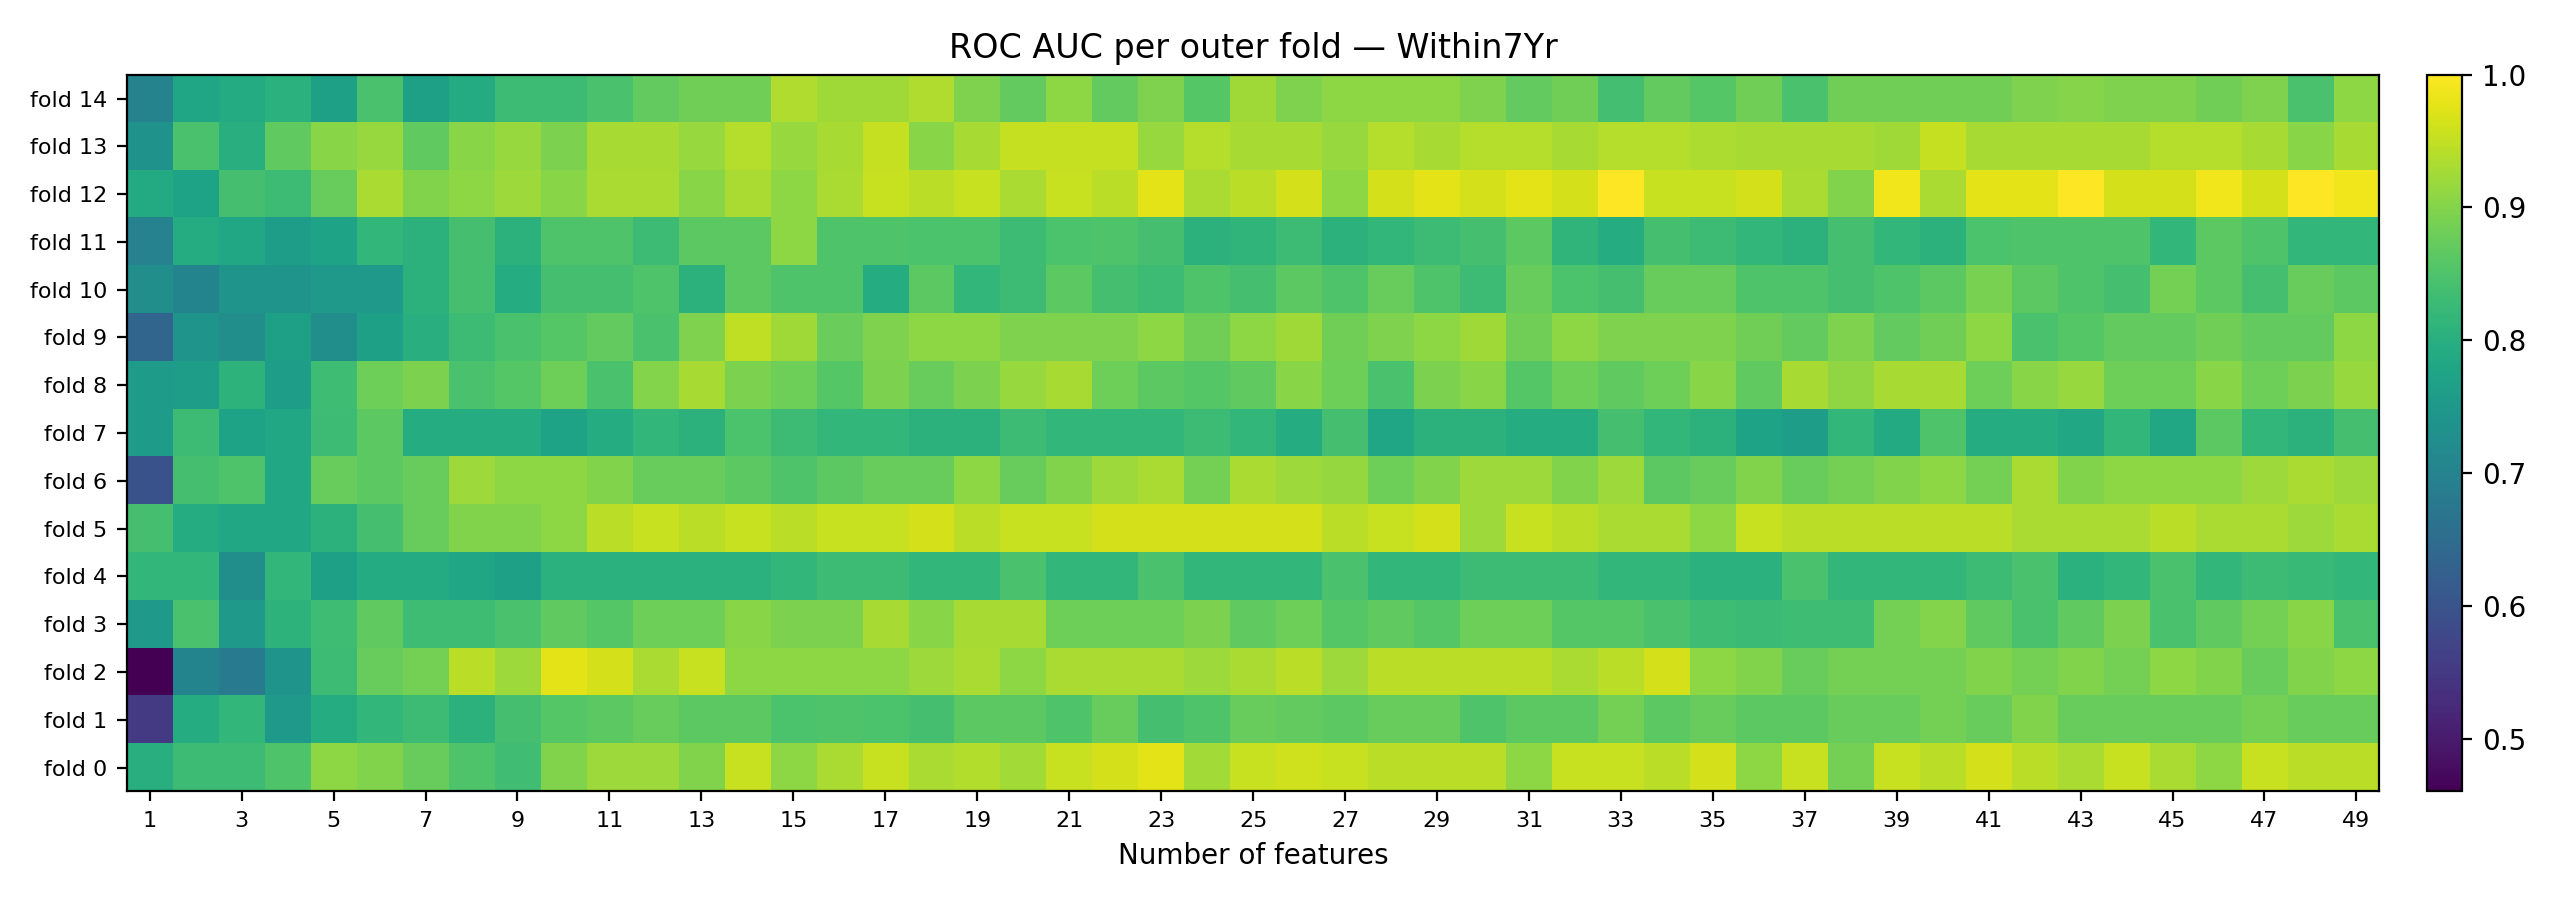
\includegraphics[width=0.85\textwidth]{gradual_heatmap_within7yr.png}
  \end{figure}
  \begin{itemize}
    \item Rows: 15 outer folds. Columns: $k=1,\dots,49$.
    \item Most variance is across folds (rows), not across $k$ within a
          fold $\Rightarrow$ slimmer signature is plausibly safe.
  \end{itemize}
\end{frame}

\begin{frame}{Within7Yr -- ranking used by the sweep}
  \begin{figure}
    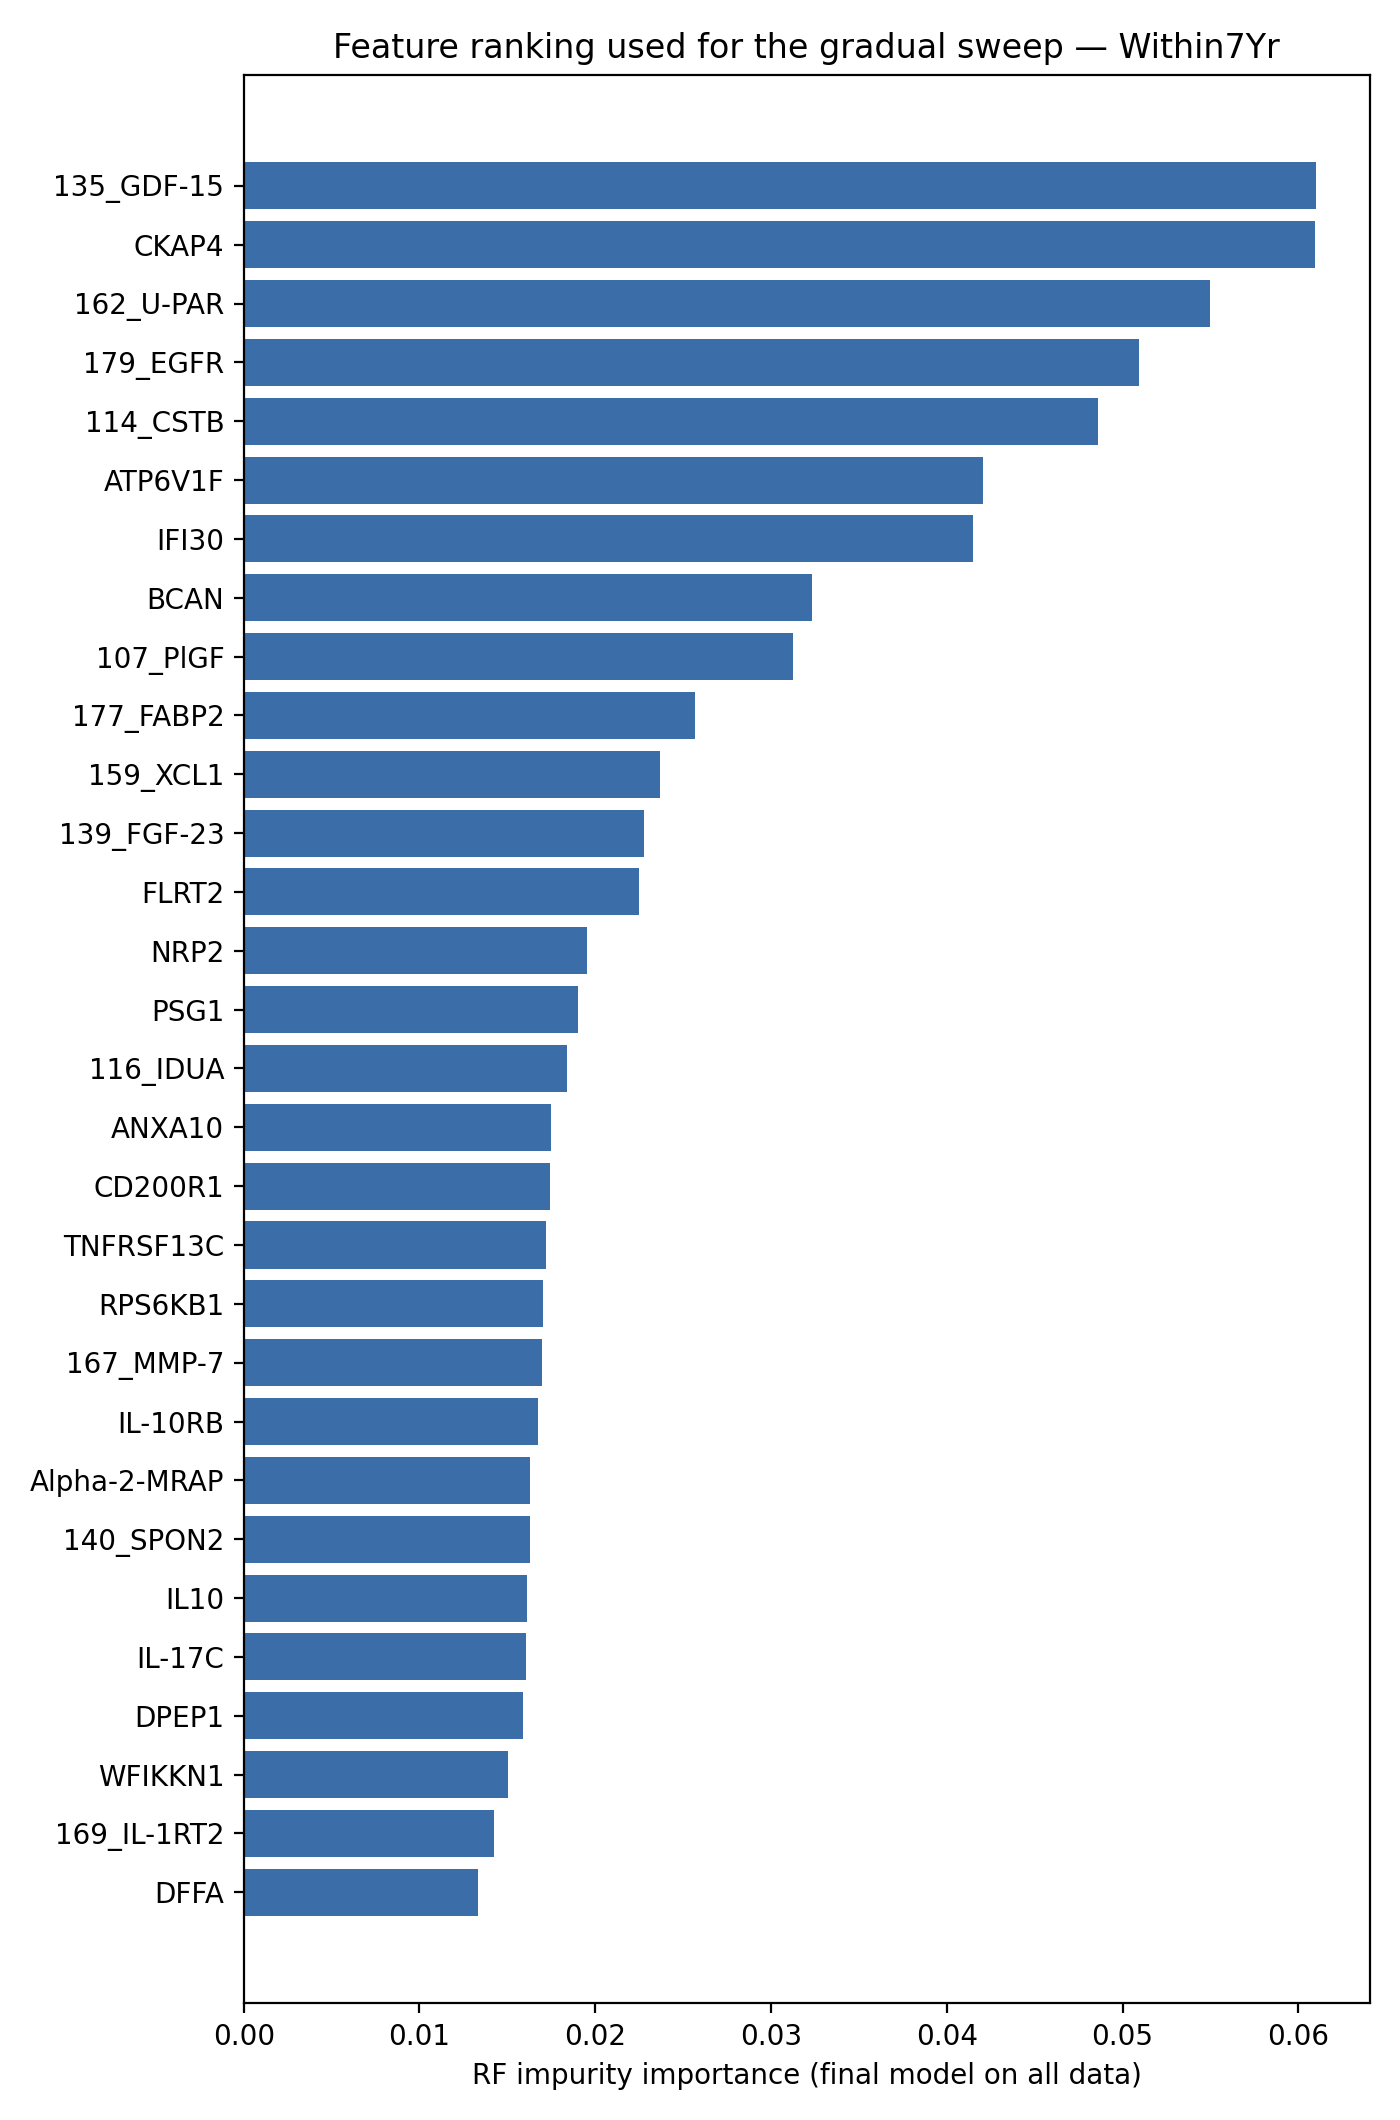
\includegraphics[width=0.85\textwidth]{gradual_features_within7yr.png}
  \end{figure}
  Order in which features enter the model as $k$ grows.
\end{frame}

% =============================================================================
\section{Cross-model gradual sweep \& the look-ahead caveat}

\begin{frame}{Gradual peaks: tree vs.\ linear/kernel}
  \begin{columns}[T]
  \column{0.55\textwidth}
    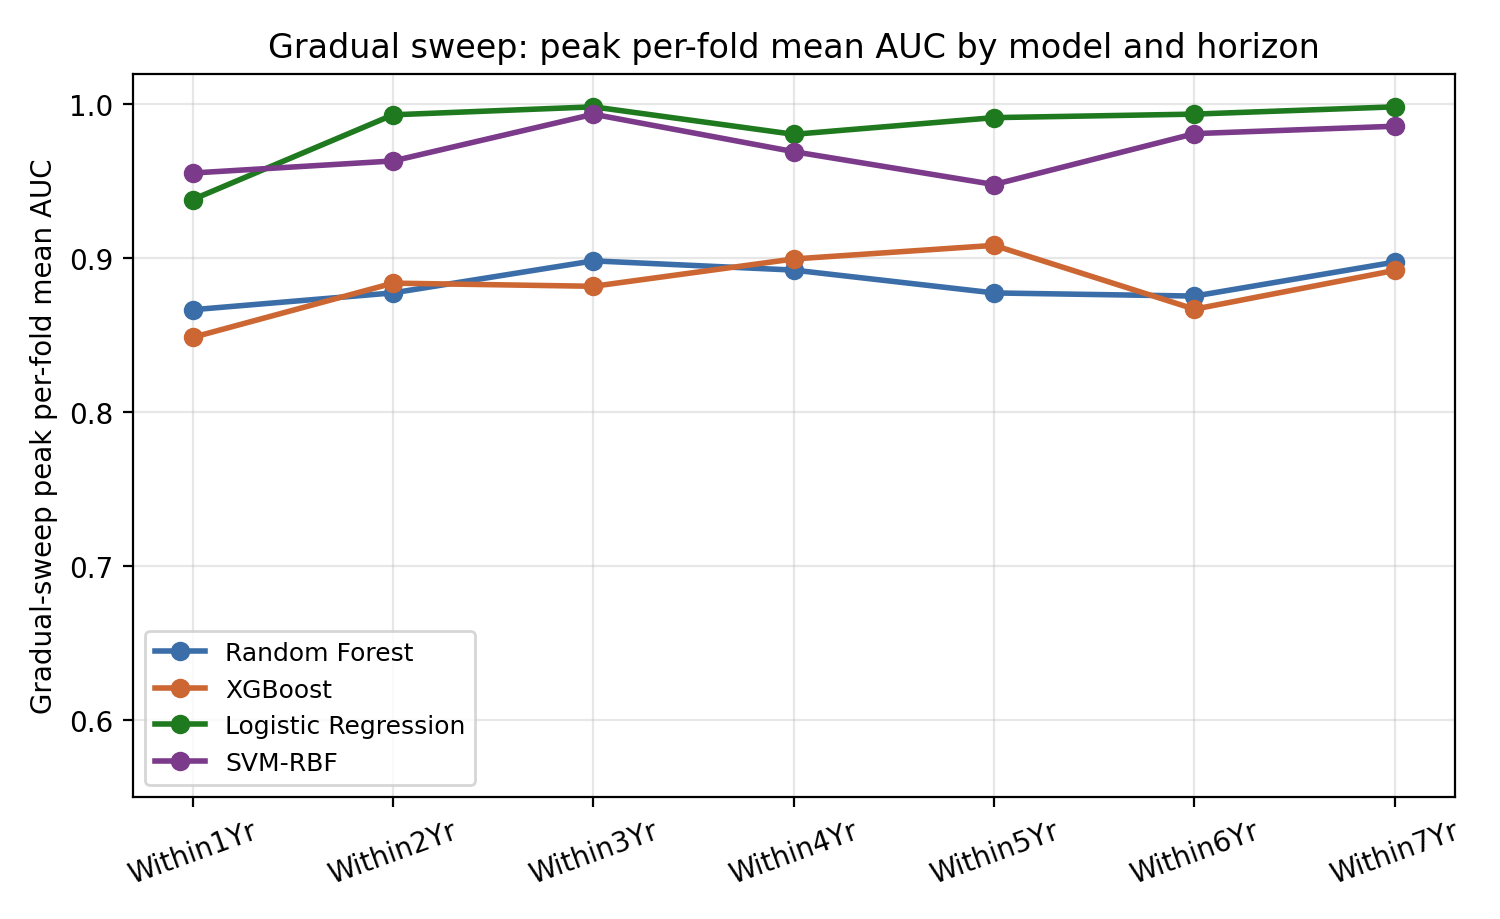
\includegraphics[width=\linewidth]{compare_models_peak_auc.png}
  \column{0.45\textwidth}
    \begin{itemize}
      \item RF / XGB: peak AUC $\sim 0.85$--$0.91$.
      \item LR / SVM-RBF: peak AUC \textbf{$\sim 0.95$--$1.00$}.
      \item LR/SVM peaks are close to perfect on every horizon.
      \item This is \textbf{not} a real predictive advantage --
            it is the rank-induced look-ahead, larger because
            $|$LR coefficient$|$ and SVM permutation importance
            are sufficient statistics of the global model.
    \end{itemize}
  \end{columns}
\end{frame}

\begin{frame}{Quantifying the look-ahead}
  \begin{columns}[T]
  \column{0.6\textwidth}
    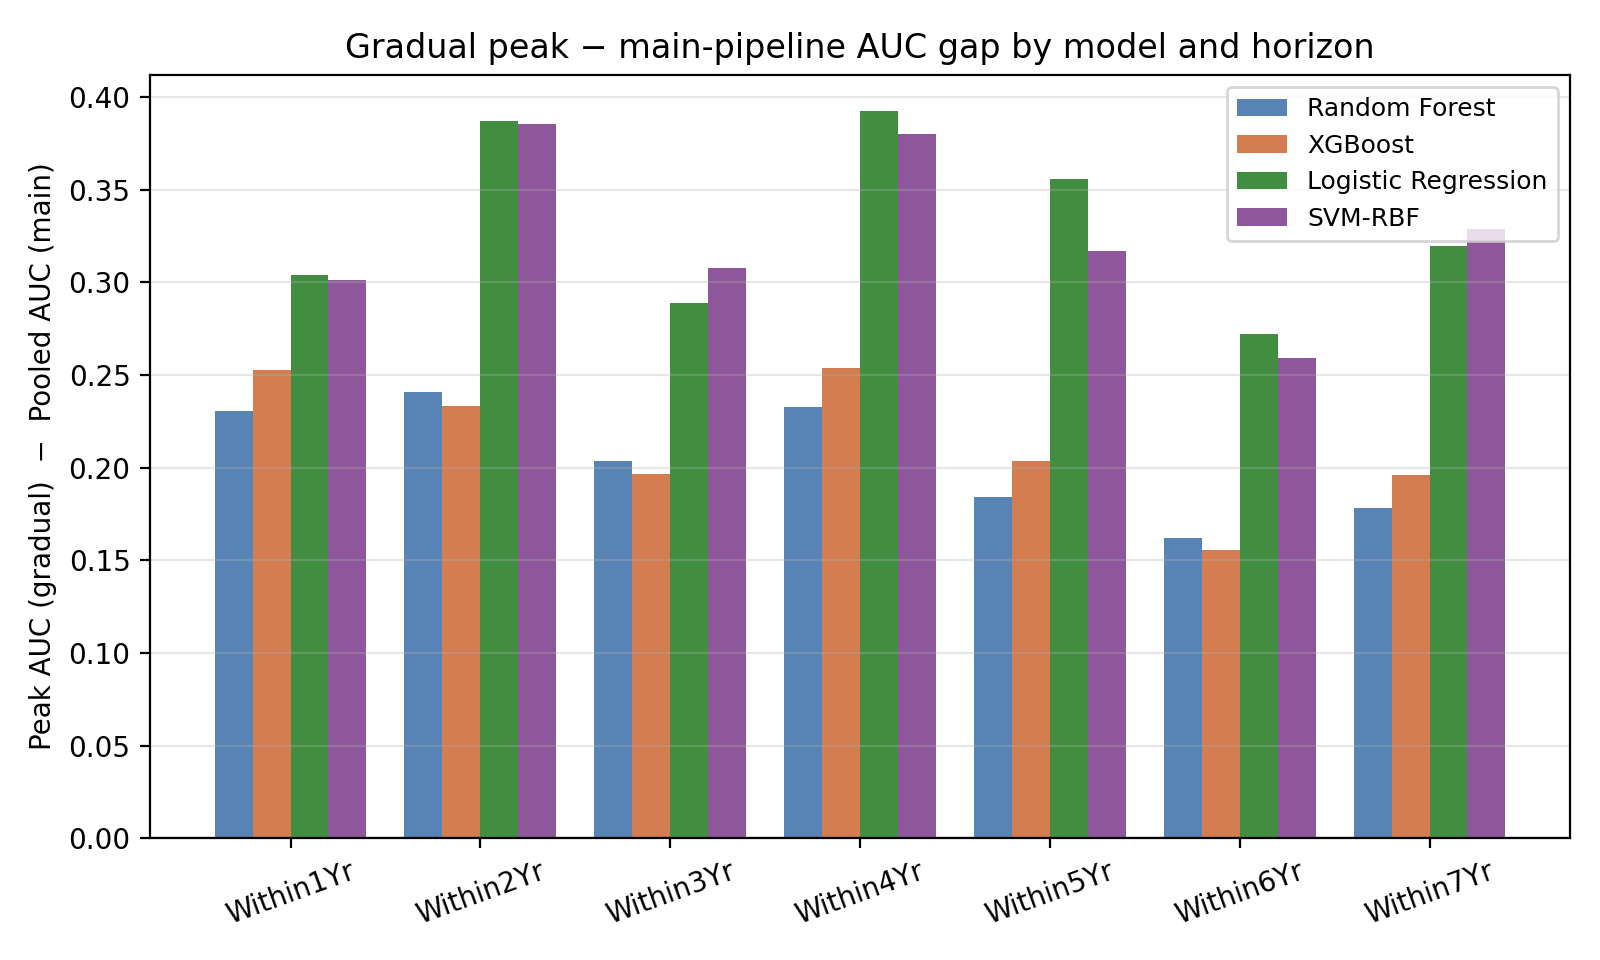
\includegraphics[width=\linewidth]{compare_models_peak_minus_pooled.png}
  \column{0.4\textwidth}
    \begin{itemize}
      \item $\Delta$ = peak (gradual) $-$ pooled (main).
      \item RF: $\Delta \approx 0.18$--$0.20$ AUC.
      \item XGB: $\Delta \approx 0.20$ AUC.
      \item LR: $\Delta \approx 0.29$--$0.32$ AUC.
      \item SVM: $\Delta \approx 0.31$--$0.33$ AUC.
    \end{itemize}
  \end{columns}
  \vspace{0.5em}
  \begin{block}{Why bigger for linear / kernel?}
    Their importance score \emph{is} the global model's decision
    function (LR coefficient, RBF permutation drop). Refitting on the
    top-$k$ recovers the global model rather than walking down a
    generic ranking.
  \end{block}
\end{frame}

\begin{frame}{Cross-model gradual peaks (representative horizons)}
  \scriptsize
  \begin{center}
  \begin{tabular}{ll rrr rrr}
    \toprule
    & & \multicolumn{3}{c}{Within3Yr} & \multicolumn{3}{c}{Within7Yr} \\
    \cmidrule(lr){3-5}\cmidrule(lr){6-8}
    Family & $|\mathcal{F}|$
           & Pool. & Peak ($k^\star$) & $\Delta$
           & Pool. & Peak ($k^\star$) & $\Delta$ \\
    \midrule
    Random Forest       & 48/49 & 0.695 & 0.898 ($k\!=\!34$) & $+0.20$ & 0.719 & 0.898 ($k\!=\!26$) & $+0.18$ \\
    XGBoost             & 48/49 & 0.685 & 0.882 ($k\!=\!31$) & $+0.20$ & 0.696 & 0.892 ($k\!=\!28$) & $+0.20$ \\
    Logistic Regression & 48/49 & 0.710 & 0.998 ($k\!=\!31$) & $+0.29$ & 0.679 & 0.998 ($k\!=\!40$) & $+0.32$ \\
    SVM-RBF             & 48/49 & 0.686 & 0.994 ($k\!=\!38$) & $+0.31$ & 0.657 & 0.986 ($k\!=\!48$) & $+0.33$ \\
    \bottomrule
  \end{tabular}
  \end{center}
  \vspace{0.6em}
  \begin{itemize}
    \item Headline numbers $\Rightarrow$ \textbf{main pipeline}.
    \item Gradual sweep $\Rightarrow$ sensitivity-on-rank;
          informative as a parsimony argument for tree models, descriptive
          only for linear/kernel.
  \end{itemize}
\end{frame}

% =============================================================================
\section{Cross-horizon synthesis}

\begin{frame}{All seven horizons at a glance}
  \begin{columns}[T]
  \column{0.5\textwidth}
    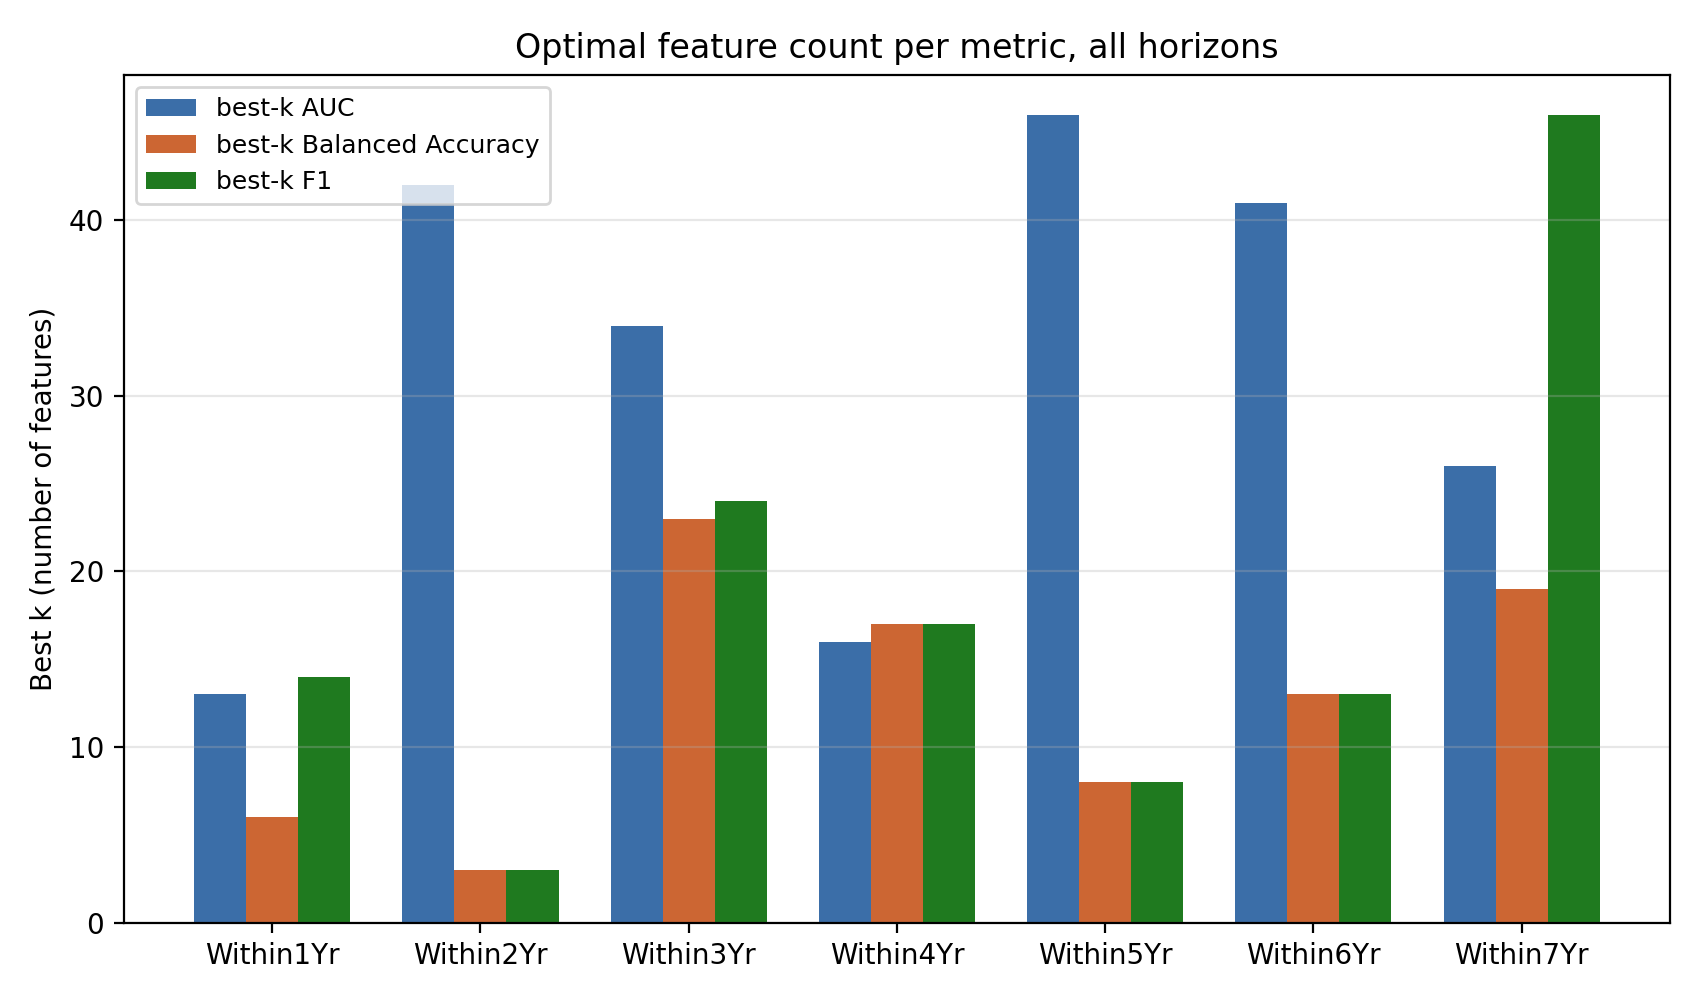
\includegraphics[width=\linewidth]{summary_best_k.png}
    \begin{center}\scriptsize Best $k$ per metric, per horizon.\end{center}
  \column{0.5\textwidth}
    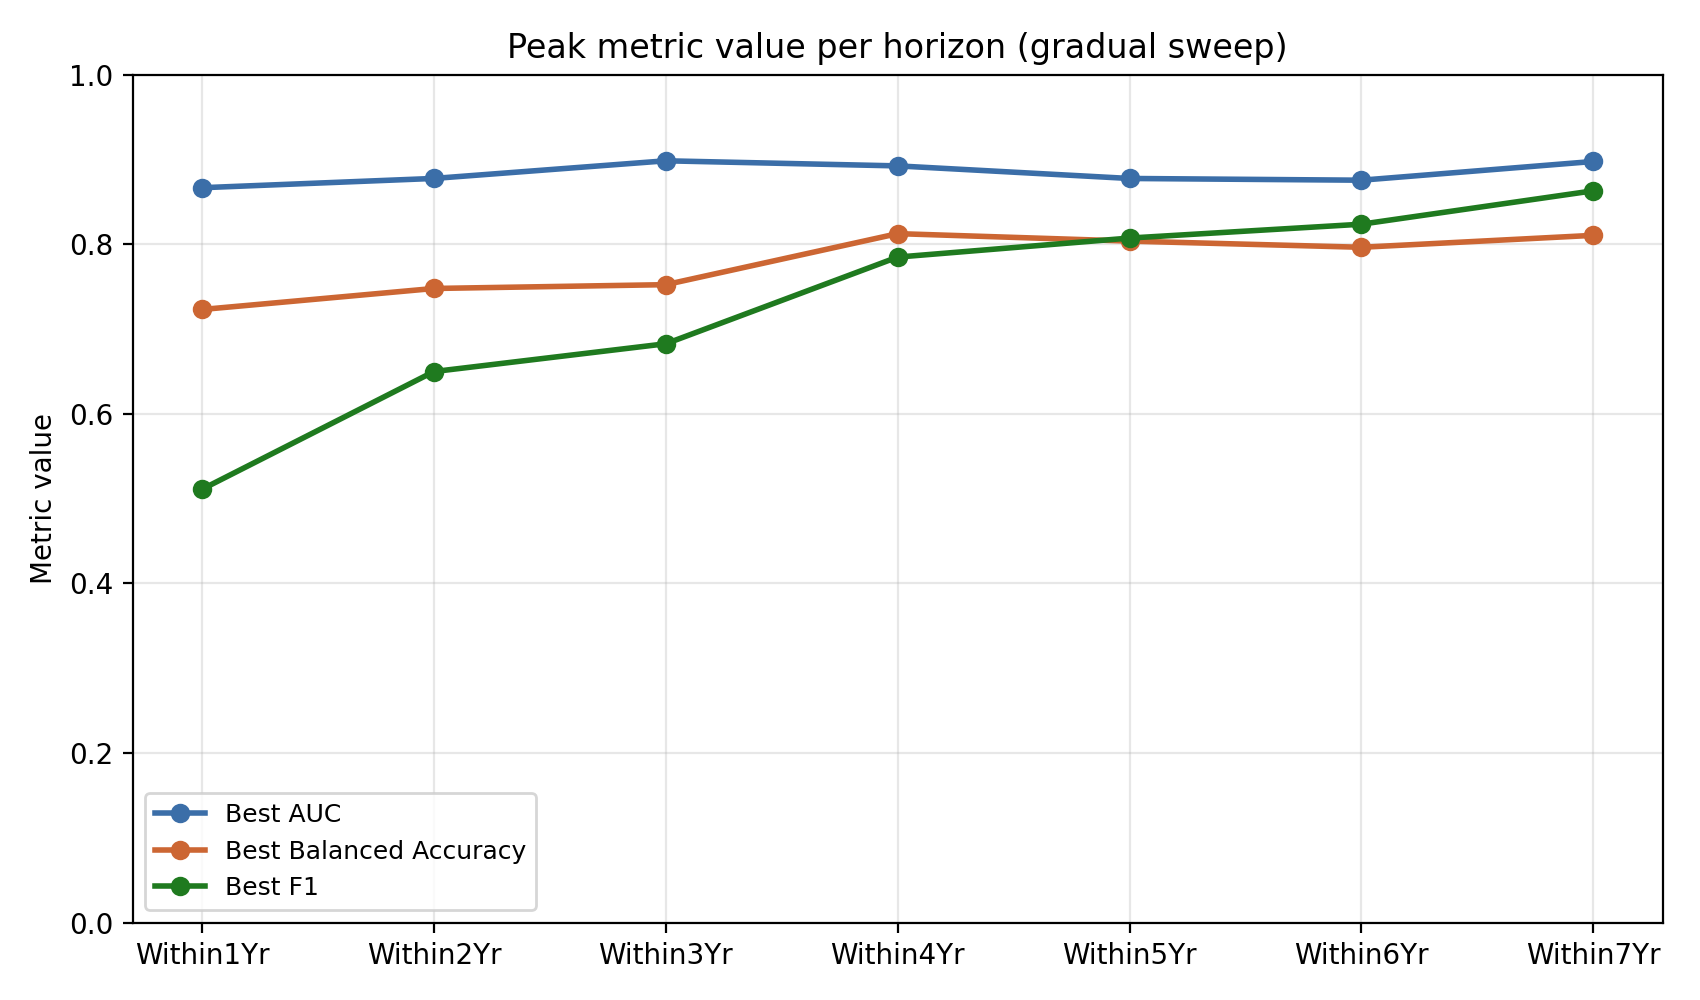
\includegraphics[width=\linewidth]{summary_best_metric_value.png}
    \begin{center}\scriptsize Peak metric value per horizon.\end{center}
  \end{columns}
  \begin{itemize}
    \item Best $k$ for AUC: 13--46 (median $\approx 34$).
    \item Best $k$ for BalAcc / $F_1$: usually \textbf{far below}
          $|\mathcal{F}|$ (often 3--25).
    \item Long, balanced horizons (Within6Yr, Within7Yr) give the best
          peaks; short, imbalanced horizons are harder.
  \end{itemize}
\end{frame}

\begin{frame}{Headline numbers across all horizons}
  \scriptsize
  \begin{center}
  \begin{tabular}{lrrrrrrr}
    \toprule
    Horizon & $|\mathcal{F}|$ & Pooled AUC & Peak AUC & $k^\star_{\mathrm{AUC}}$
            & Peak BalAcc & $k^\star_{\mathrm{BalAcc}}$ & Peak $F_1$\\
    \midrule
    Within1Yr & 33 & 0.636 & 0.867 & 13 & 0.723 &  6 & 0.511 \\
    Within2Yr & 50 & 0.637 & 0.878 & 42 & 0.748 &  3 & 0.650 \\
    Within3Yr & 48 & 0.695 & 0.898 & 34 & 0.752 & 23 & 0.683 \\
    Within4Yr & 38 & 0.660 & 0.892 & 16 & 0.813 & 17 & 0.785 \\
    Within5Yr & 46 & 0.693 & 0.878 & 46 & 0.804 &  8 & 0.807 \\
    Within6Yr & 50 & 0.714 & 0.876 & 41 & 0.796 & 13 & 0.824 \\
    \textbf{Within7Yr} & 49 & 0.719 & \textbf{0.898} & 26 & \textbf{0.810} & 19 & 0.863 \\
    \bottomrule
  \end{tabular}
  \end{center}
  \begin{itemize}
    \item Pooled = main pipeline (full $|\mathcal{F}|$); Peak = gradual sweep.
    \item Gap between pooled and peak suggests \textbf{a slimmer
          signature would beat the published list}.
  \end{itemize}
\end{frame}

% =============================================================================
\section{Discussion}

\begin{frame}{What the cross-model story tells us}
  \begin{itemize}
    \item \textbf{Headline AUC is data-limited:} four families,
          $\sim 0.06$ AUC of spread, smaller than the per-fold SD.
    \item \textbf{Tree models lead at long, balanced horizons; linear
          / kernel models match at the short, imbalanced one.}
    \item \textbf{Tree-model gradual sweeps} are an honest parsimony
          argument: peak well before $|\mathcal{F}|$, with a $\sim
          0.18$--$0.20$ rank-induced lift over pooled.
    \item \textbf{Linear / kernel gradual sweeps} should be read as a
          description of the published ranking only --- their peaks
          near $1.0$ are the global model leaking into its own
          ranking.
  \end{itemize}
  \begin{block}{Caveats on optimism}
    Choosing the $k$ that maximises a sample-mean curve is itself a model
    selection step. Reported peaks are ``best achievable along this
    published ranking'', not deployment estimates.
  \end{block}
\end{frame}

\begin{frame}{Limitations}
  \begin{itemize}
    \item \textbf{Sample size.} $n=94$ for $551$ features.
          $\pm 1$\,SD bands are wide -- adjacent points on the
          $k$-curve are not statistically distinguishable.
    \item \textbf{Single cohort.} No external validation cohort
          available yet -- the most important next step.
    \item \textbf{Binary horizons.} Cox / discrete-time-survival
          reformulation would account for censoring properly.
    \item \textbf{Calibration.} Brier reported, but no Platt / isotonic
          recalibration applied.
    \item \textbf{Calibration disparity.} LR / SVM-RBF have similar AUC
          to RF / XGB but worse Brier; Platt or isotonic recalibration
          is the next step.
    \item \textbf{Rank-on-full-data look-ahead.} Tree-importance
          rankings: small bias. Linear / kernel rankings: large bias
          $\Rightarrow$ gradual sweep is descriptive only for those
          families.
  \end{itemize}
\end{frame}

% =============================================================================
\section{Conclusions}

\begin{frame}{Take-home messages}
  \begin{enumerate}
    \item A leakage-free, nested-CV, stability-selected \textbf{four-family}
          pipeline (RF, XGB, LR, SVM-RBF) gives \textbf{honest held-out
          AUC of 0.60--0.72} across the 1--7 year horizons.
    \item The four families are within $\sim 0.06$ AUC of one another at
          every horizon: \textbf{headline performance is data-limited,
          not model-limited.}
    \item Random Forest is the anchor model: pooled AUC $0.719$ at
          Within7Yr; peak gradual AUC $0.898$ at $k=26$;
          peak balanced accuracy $0.810$ at $k=19$.
    \item \textbf{Parsimony argument} (tree models): held-out
          performance plateaus well before $|\mathcal{F}|$ -- a slimmer
          interpretable signature is plausible.
    \item \textbf{Rank-induced look-ahead}: LR / SVM-RBF gradual peaks
          near $1.0$ are an artefact of using the global model's own
          importance as a ranking; main-pipeline numbers are the
          headline.
    \item Reproducible from a single fixed seed (\texttt{RANDOM\_STATE=42}).
  \end{enumerate}
\end{frame}

\begin{frame}{Reproducibility \& code}
  \begin{itemize}
    \item Single \texttt{RANDOM\_STATE = 42} propagated throughout.
    \item Four parallel pipelines, identical layout:
      \begin{itemize}
        \scriptsize
        \item \texttt{Random\_Forest/src/train\_rf.py}
        \item \texttt{XGBoost/src/train\_xgb.py}
        \item \texttt{LogisticRegression/src/train\_lr.py}
        \item \texttt{SVM/src/train\_svm.py}
        \item plus matching \texttt{src\_gradual\_training/gradual\_train.py}
              under each.
      \end{itemize}
    \item Outputs: \texttt{<Model>/results/} and
          \texttt{<Model>/results\_gradual\_training/}.
    \item Per-horizon artefacts: \texttt{metrics.json},
          \texttt{cv\_predictions.csv}, \texttt{model.joblib}, plots.
  \end{itemize}
  \vspace{1em}
  \begin{center}
    \Large Thank you. Questions?
  \end{center}
\end{frame}

\end{document}
